% !TEX root = trkjet.tex

This section further discusses results from the previous section.

%%cent dependence
The centrality dependence of \RDptr\ for two charged-particle \pt\ intervals: 1.0--1.6~\GeV\ and \mbox{6.3--10.0~\GeV}, and two different \ptjet\ ranges: 126--158~\GeV\ and 200--251~\GeV, is presented in Figure~\ref{fig:centdep}. 
For both \ptjet\ selections and  1.0--1.6~\GeV\ charged particles, the magnitude of the excess increases
with increasing collisions centrality and with \rvar\, for \rvar\ inside the jet cone for $\rvar < 0.3$.  The magnitude of the excess is
approximately a factor of two in the most central collisions for $\rvar >$~0.3.
A continuous centrality dependent suppression of  yields of charged-particles with $6.3 < \pt < 10.0$ GeV is observed.
%With the same \ptjet\ selections and 
%charged-particles with 6.3~$ < \pt < $~10.0~\GeV a clear ordering in centrality is observed with
%the most central collisions exhibiting the smallest \RDptr\ values.
The magnitude of modifications decreases with decreasing collision centrality for both pT intervals and two pTjet selections across the entire r < 0.8 range

%The magnitude of both modifications decreases in 60--80\% central collisions for both \pt\ ranges, across the entire $ r < 0.8$ range under investigation.  
The \ptjet\ dependence of the \RDptr\ ratios is presented in Figure~\ref{fig:ptjetdep} for the 0--10\% most central collisions and two pT selections.
  A trend of increasing \RDptr\ with increasing \ptjet\ is observed for $r < 0.25$ for low 
\pt\ charged particles. 
For the higher-\pt\ charged particles, no significant dependence on \ptjet\ is observed. 

\begin{figure}[h]
\centerline{
         \begin{tabular}{cc}
%            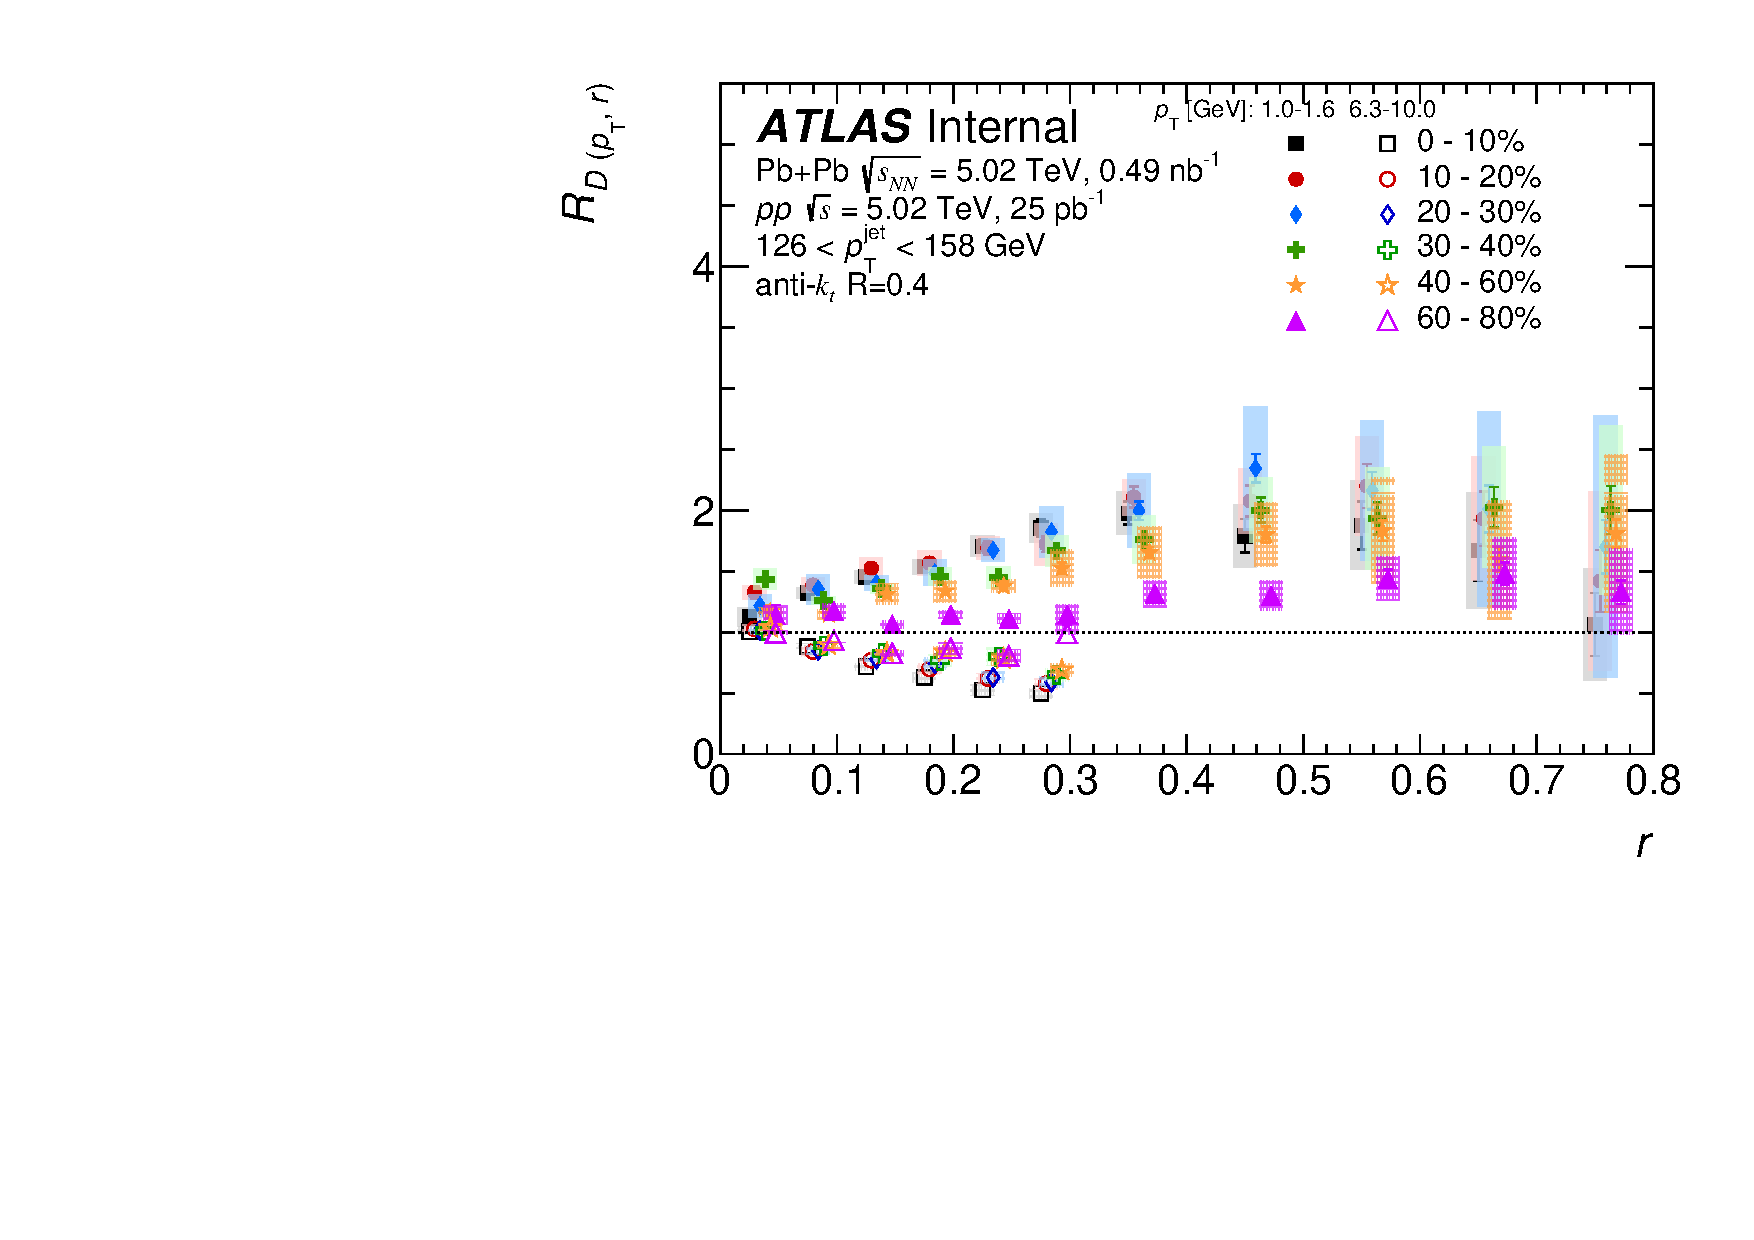
\includegraphics[width=0.5\textwidth]{figures/results/RDpT_dR_trk2_trk6_jet7.pdf} & 
%            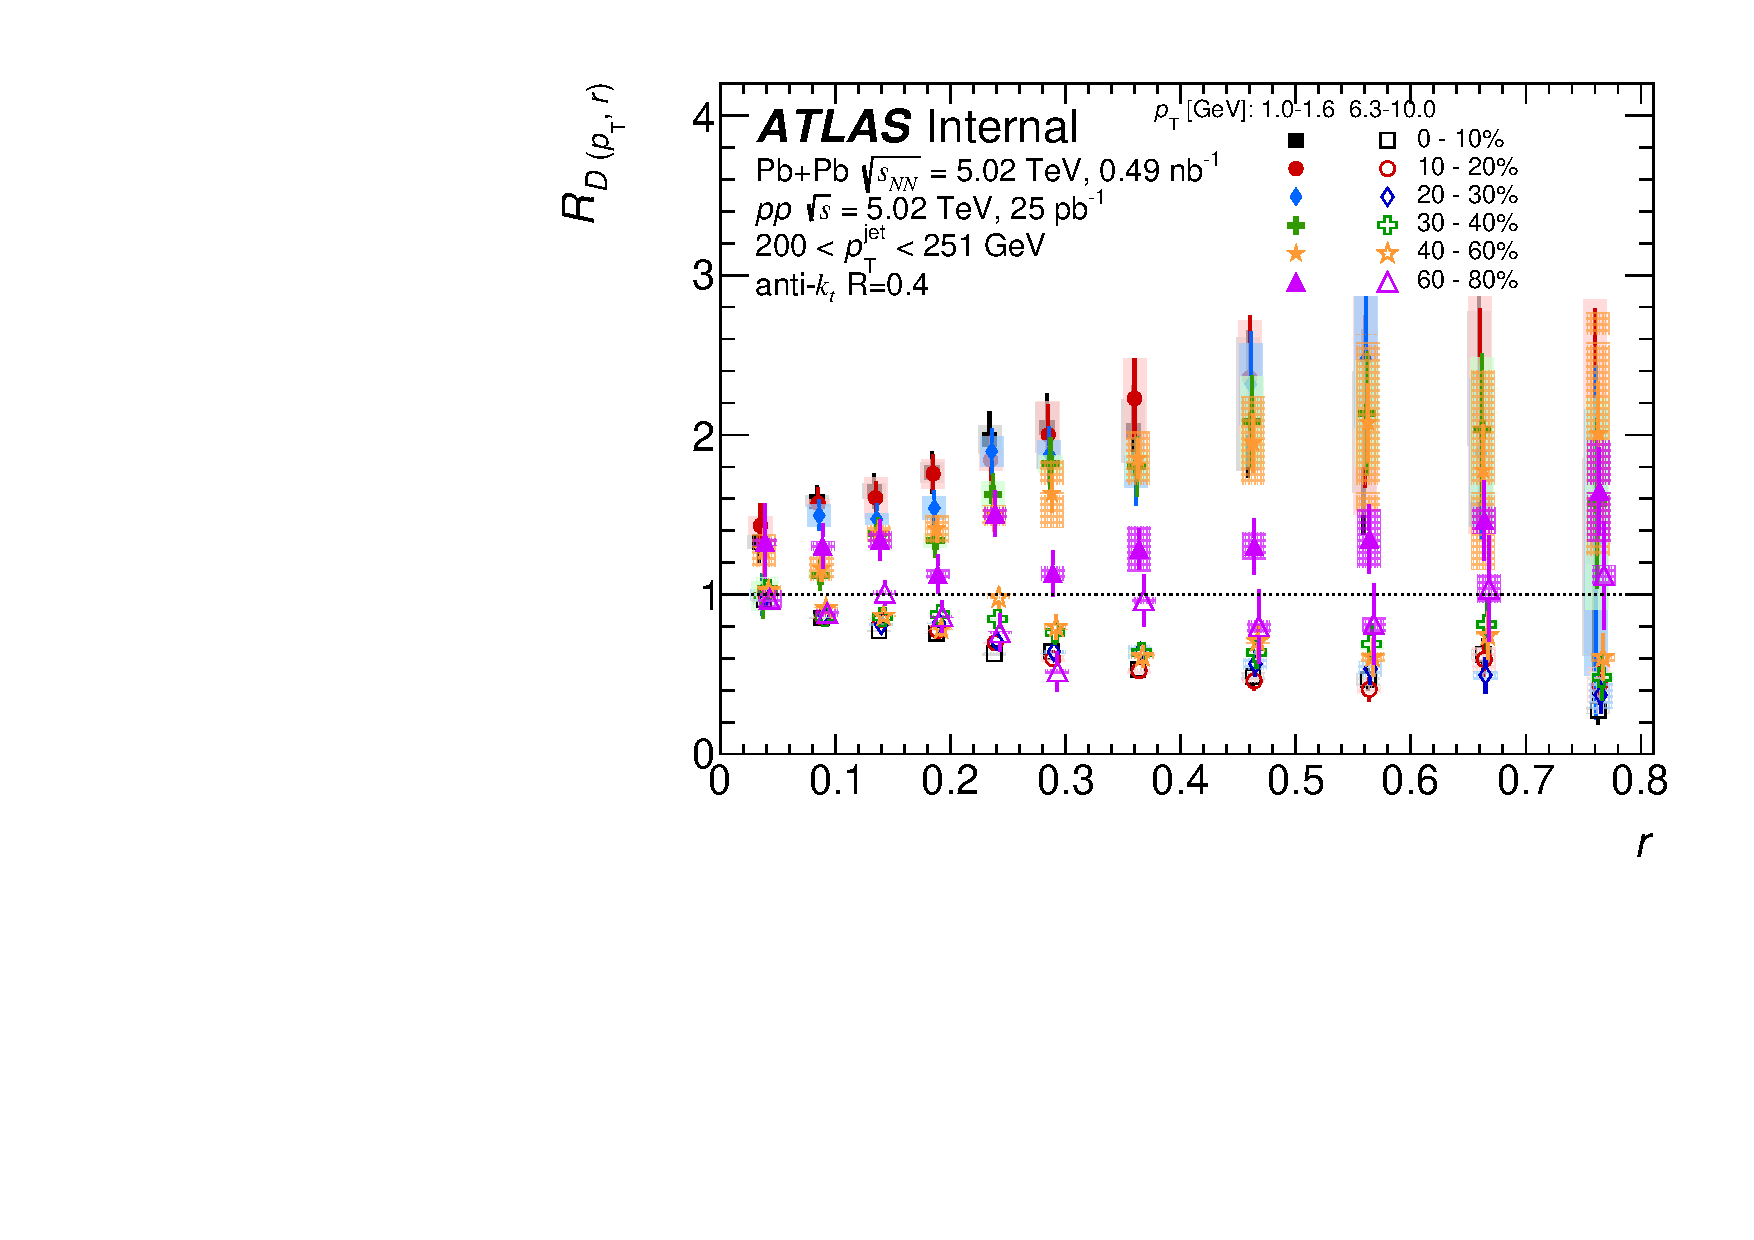
\includegraphics[width=0.5\textwidth]{figures/results/RDpT_dR_trk2_trk6_jet9.pdf} \\
            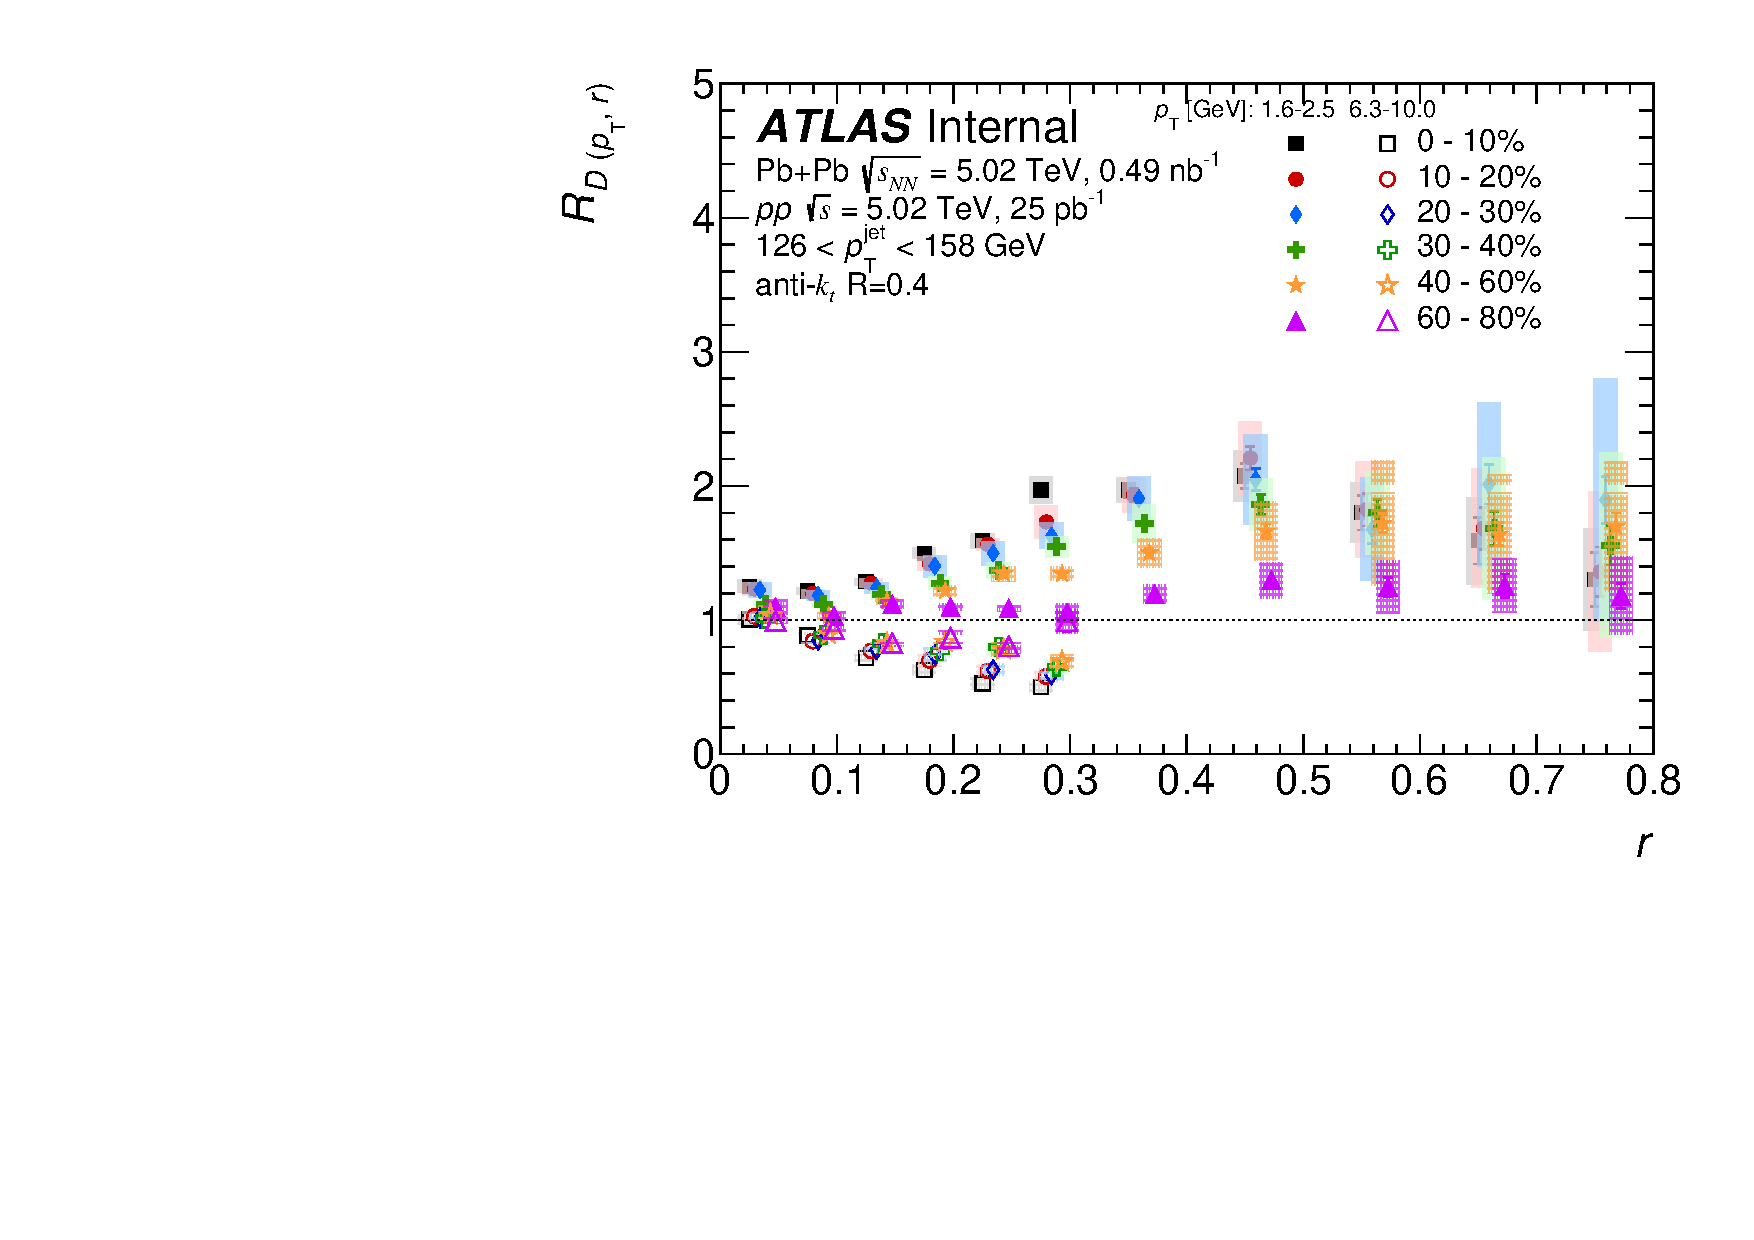
\includegraphics[width=0.5\textwidth]{figures/results/RDpT_dR_trk3_trk6_jet7.pdf} & 
            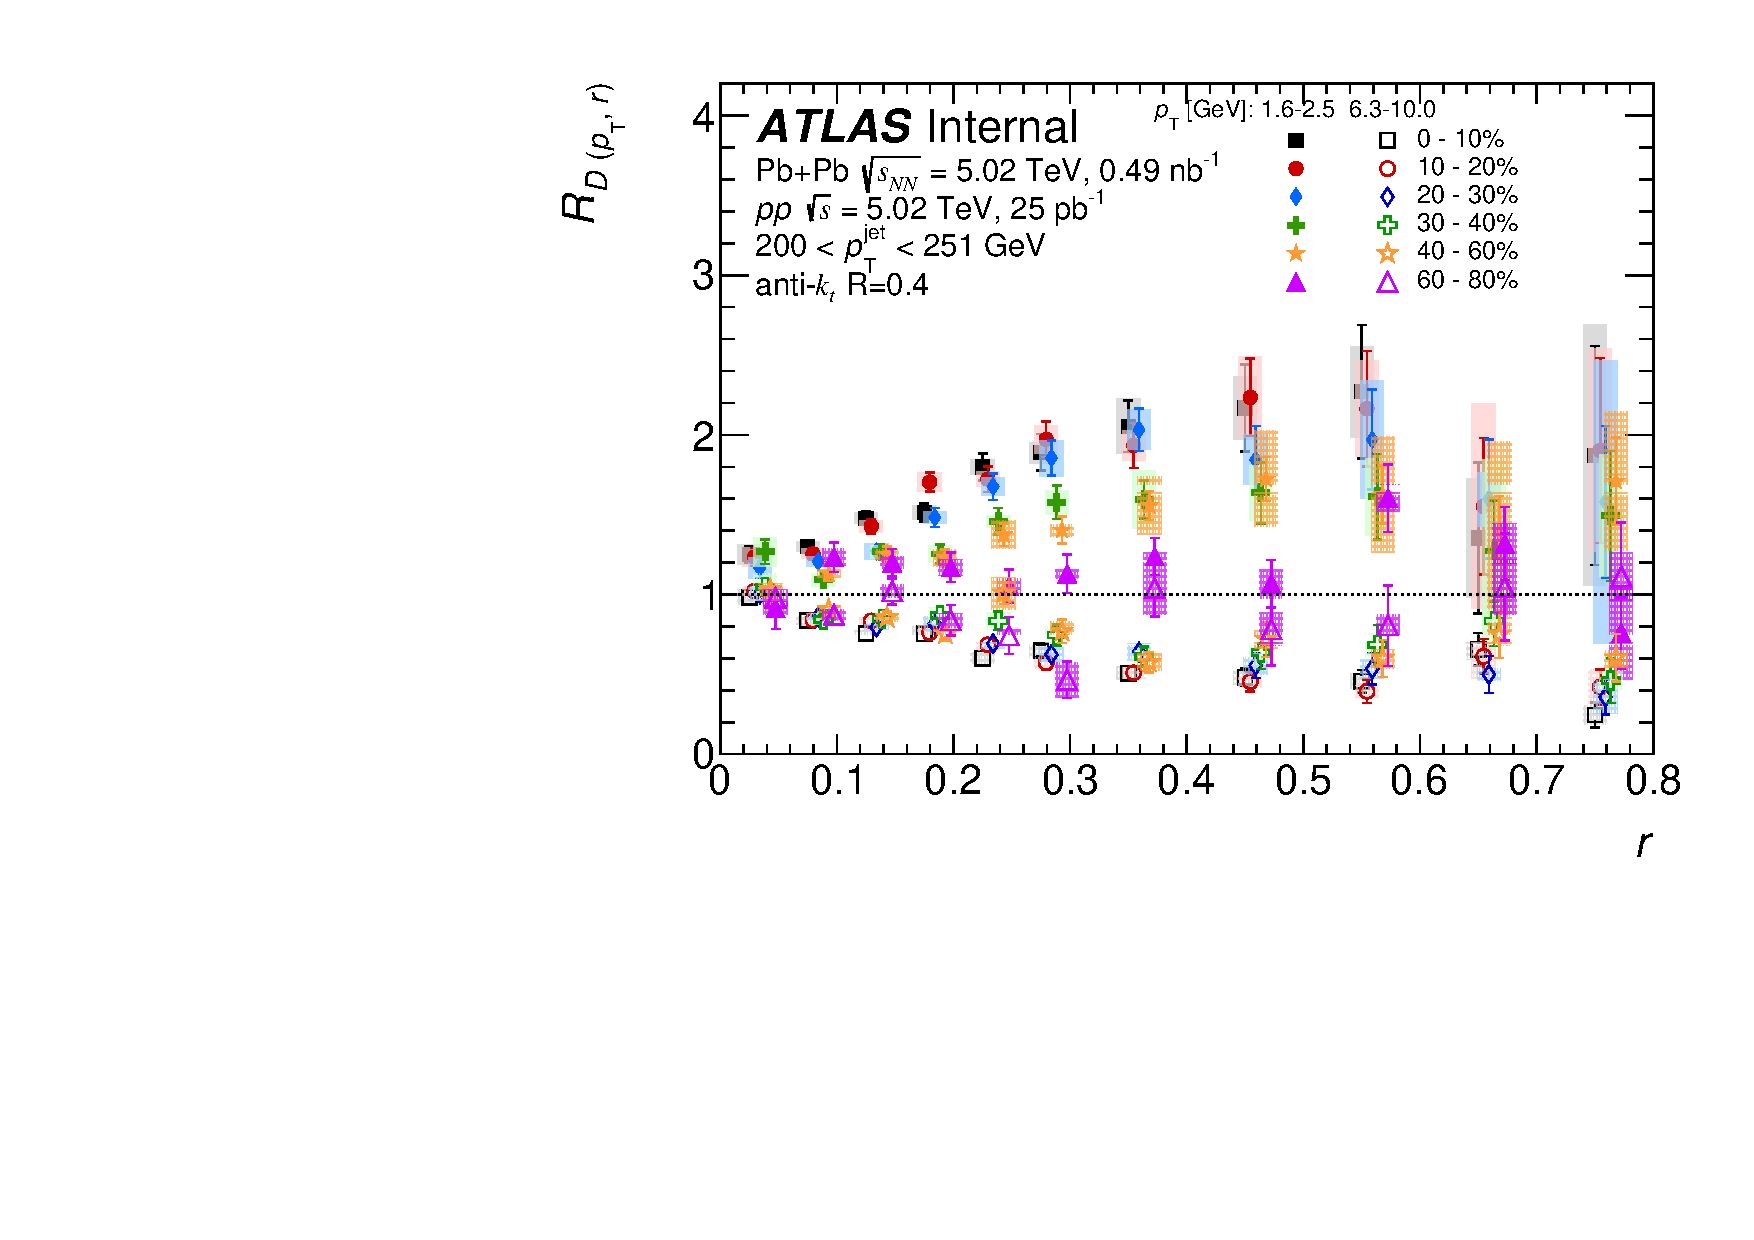
\includegraphics[width=0.5\textwidth]{figures/results/RDpT_dR_trk3_trk6_jet9.pdf} \\
      \end{tabular}
      }
   \caption{The \RDptr\ distributions for \ptjet\ of 126--158~\GeV\ and 200--251~\GeV\ as a function of angular distance $r$ for two \pt\ selections, 1.6--2.5~\GeV\ (closed symbols) and 6.3--10.0~\GeV\ (open symbols), and six centrality intervals. The vertical bars on the data points indicate statistical uncertainties while the shaded boxes indicate systematic uncertainties. The widths of the boxes are not indicative of the bin size and the points are shifted horizontally for better visibility.}
\label{fig:centdep}
\end{figure}
%%%%%%%%%%%%%

%%pt jet dependence

\begin{figure}[ht]
\centerline{
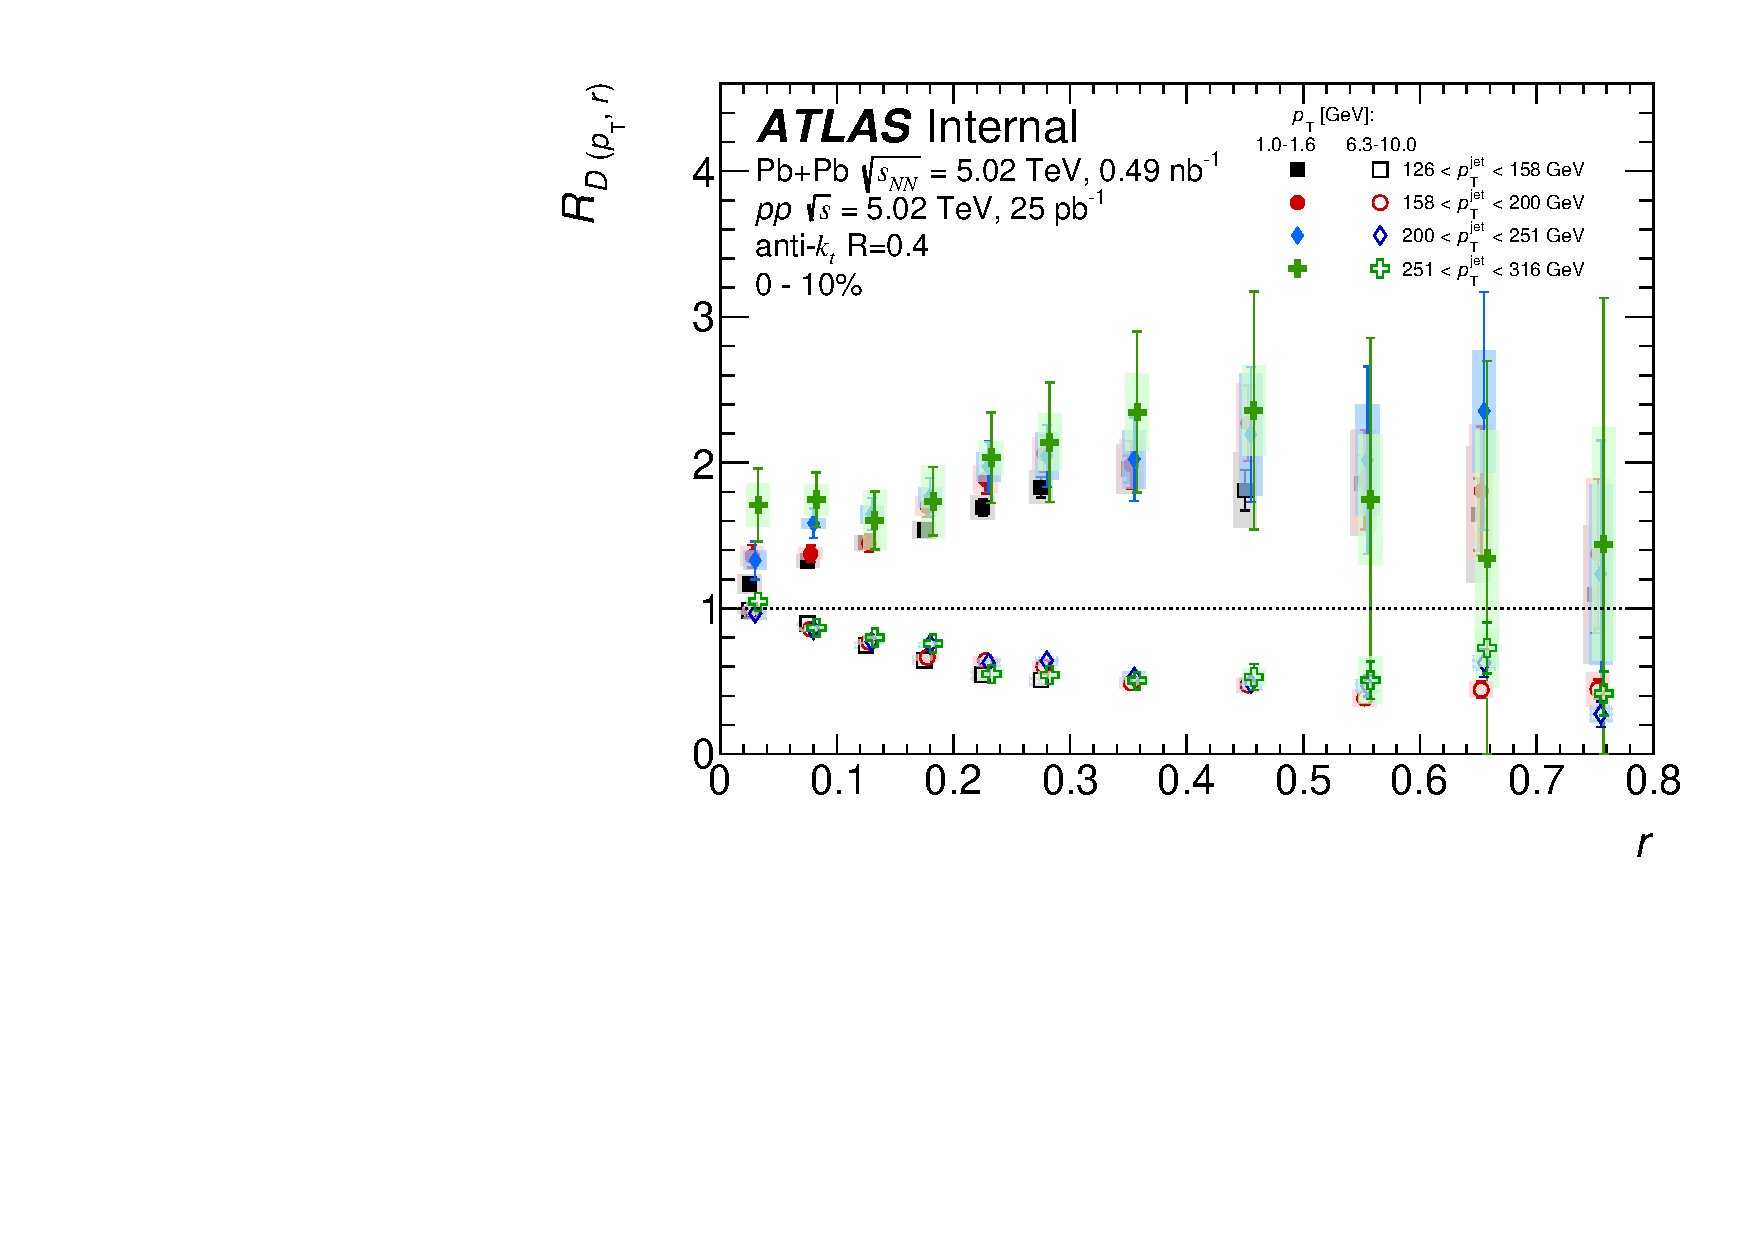
\includegraphics[width=0.8\textwidth]{figures/results/RDpT_dR_trk2_trk6_cent0.pdf} 
}
\caption{\RDptr\ as a function of \rvar\ for 0--10\% collisions for charged particles with 1.0~$< \pt <$~1.6~\GeV\
(closed symbols) and 6.3~$< \pt <$10.0~\GeV\ (open symbols) for different \ptjet\ selections. The vertical bars on the data points indicate statistical uncertainties while the shaded boxes indicate systematic uncertainties. The widths of the boxes are not indicative of the bin size and the points are shifted horizontally for better visibility.}
\label{fig:ptjetdep}
\end{figure}
%%%%%%%%%%%%%


%%pt track dependence
The charged particle \pt\ dependence of \RDptr\ for \mbox{$126 < \ptjet < 158$ GeV} and \mbox{$200 < \ptjet < 251$ GeV} for several angular distances from the jet axis in 0--10\% central and 60--80\% peripheral collisions is presented in Figure~\ref{fig:pttrkdep}. The yield of charged particles with $\pt < 4$ GeV is enhanced for $\rvar < 0.05$, along with no significant modifications for higher \pt\ charged particles. 
%No suppression is observed for $r < 0.05$ across the entire \pt\ range under investigation.
% This can also be seen in Figure~\ref{fig:rdptr} and Figure~\ref{fig:rdptr_trk_cent}, where any suppression in the charged particle spectra is at distances larger than $r = 0.05 $ 
%from the jet axis. 

\begin{figure}
\centering{
\begin{tabular}{cc}
	 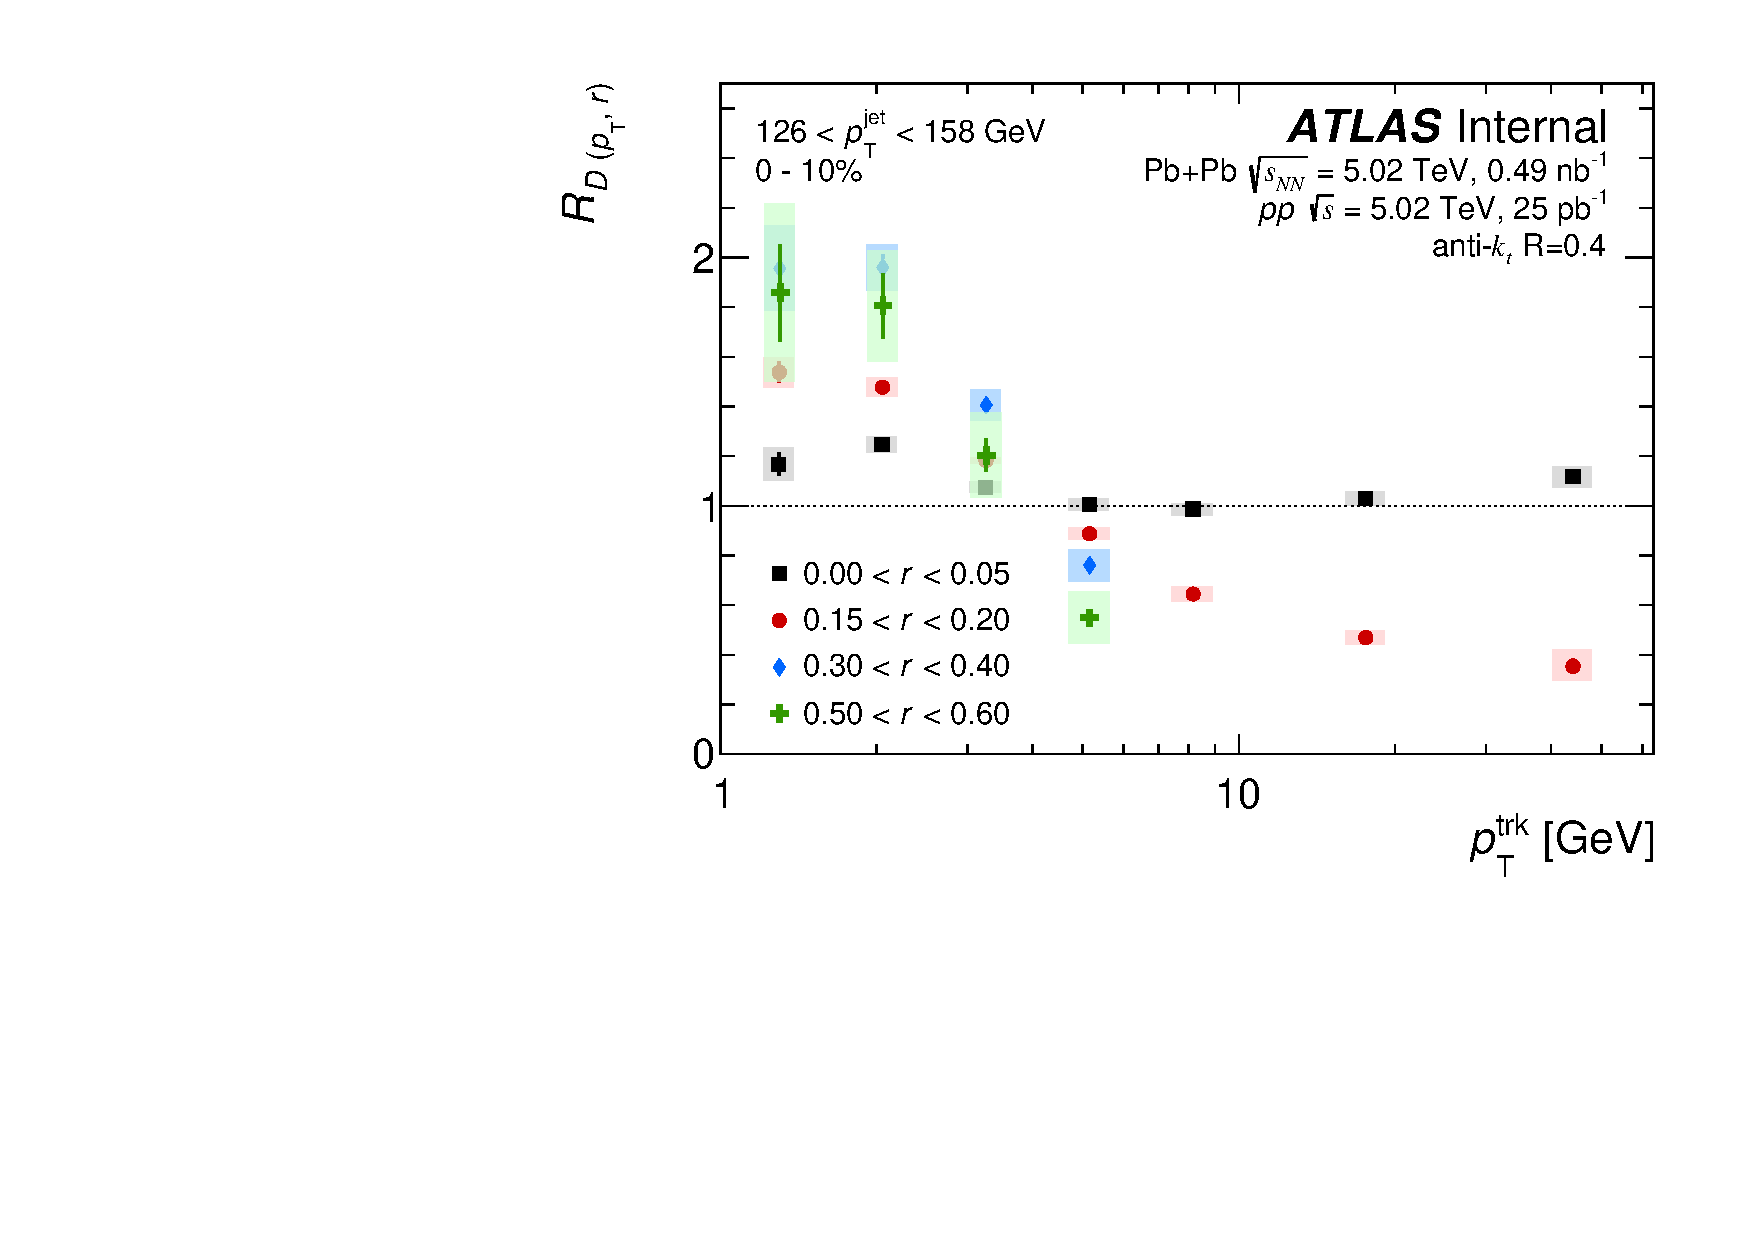
\includegraphics[width=0.5\textwidth]{results/RDpT_trkpt_jet7_cent0} &
	 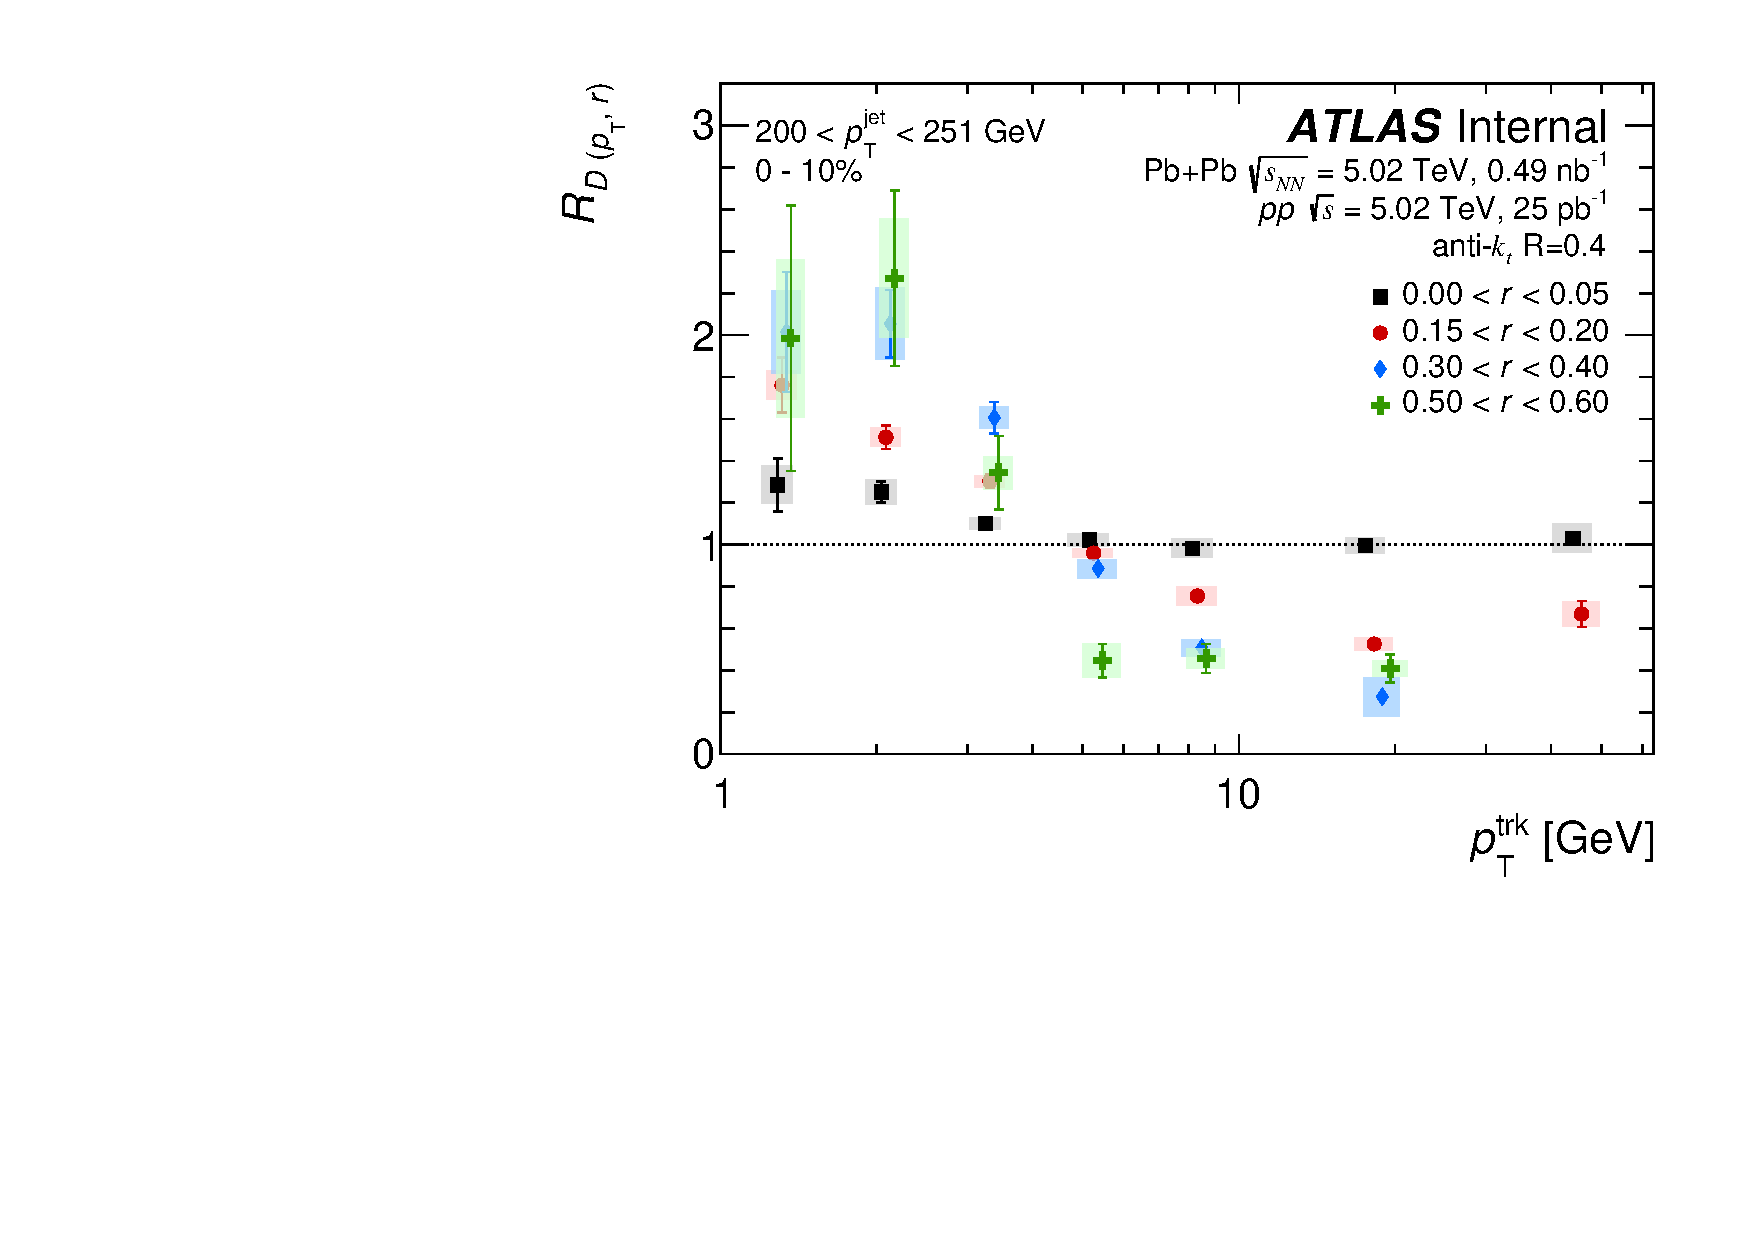
\includegraphics[width=0.5\textwidth]{results/RDpT_trkpt_jet9_cent0} \\
	 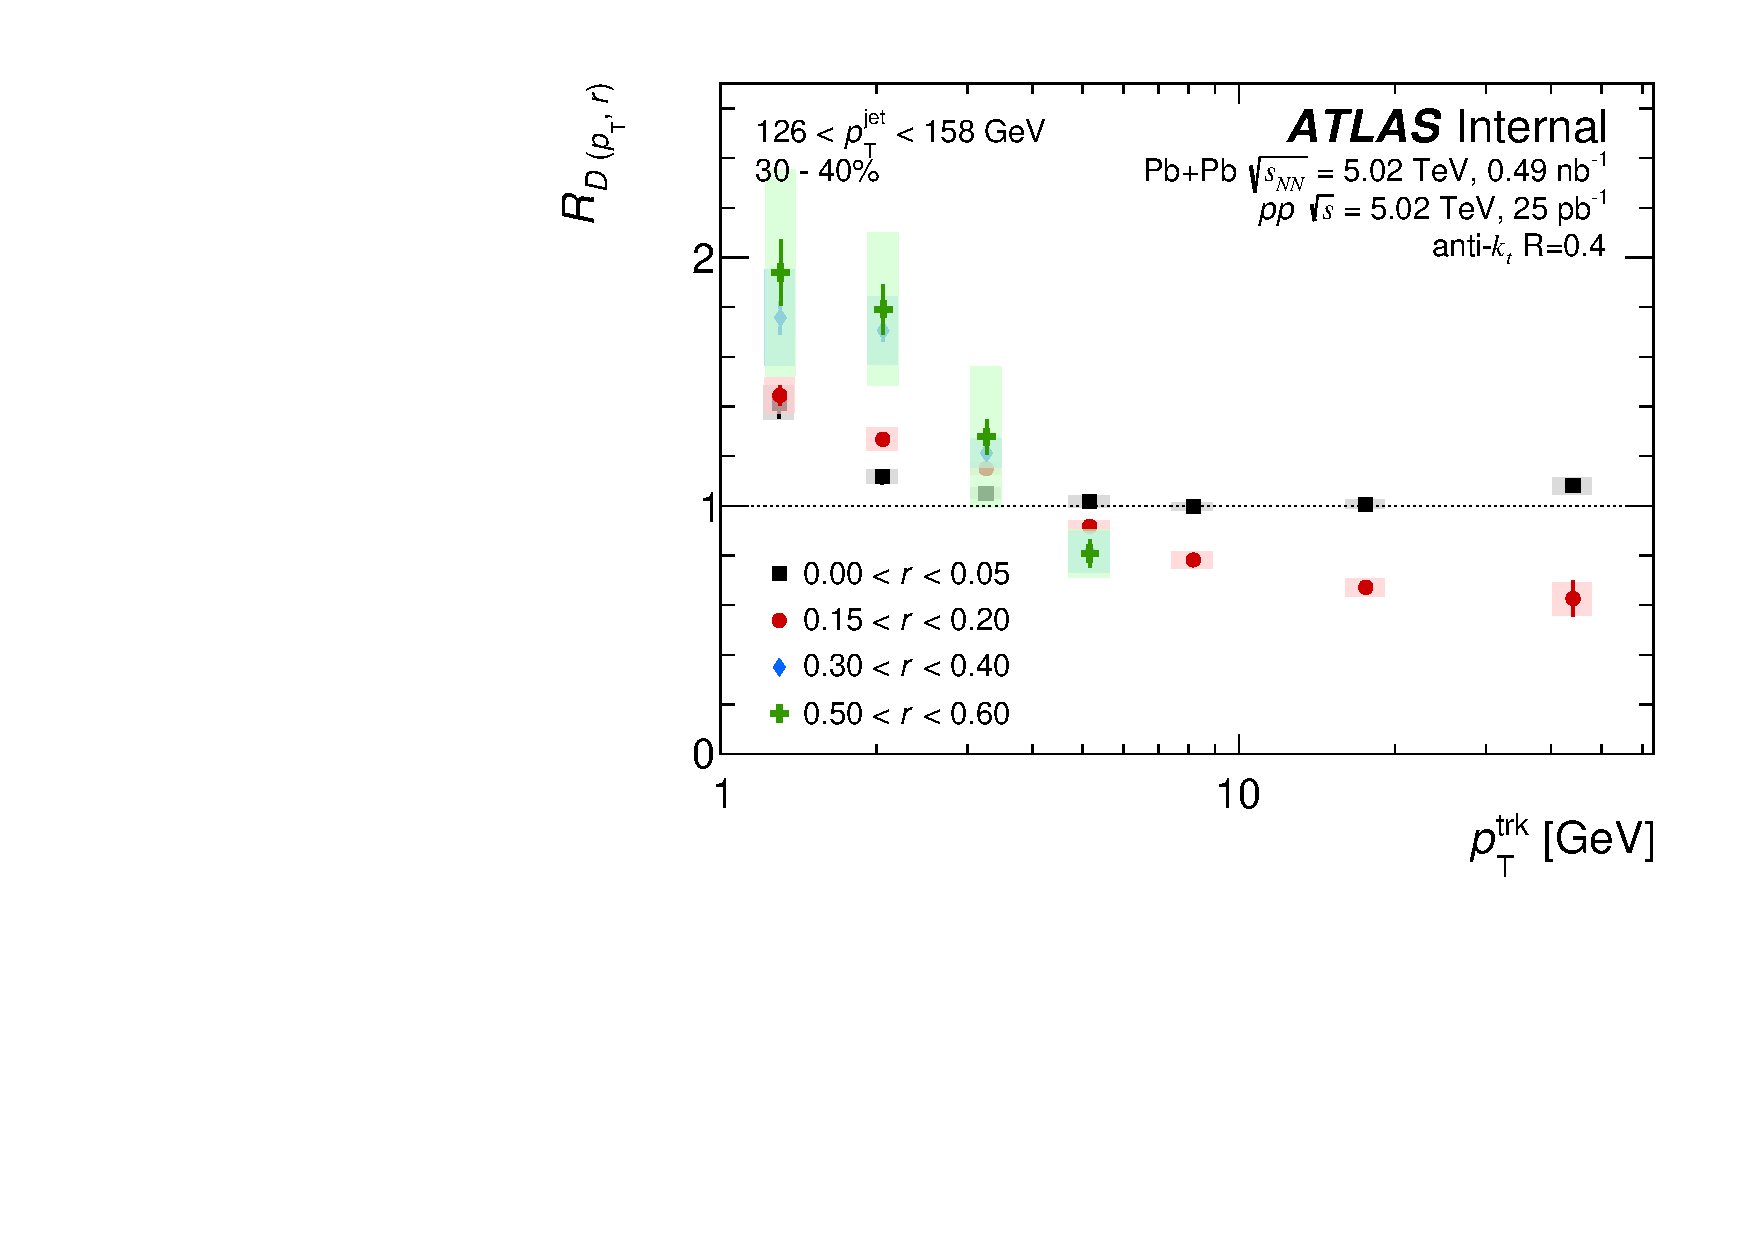
\includegraphics[width=0.5\textwidth]{results/RDpT_trkpt_jet7_cent3} &
	 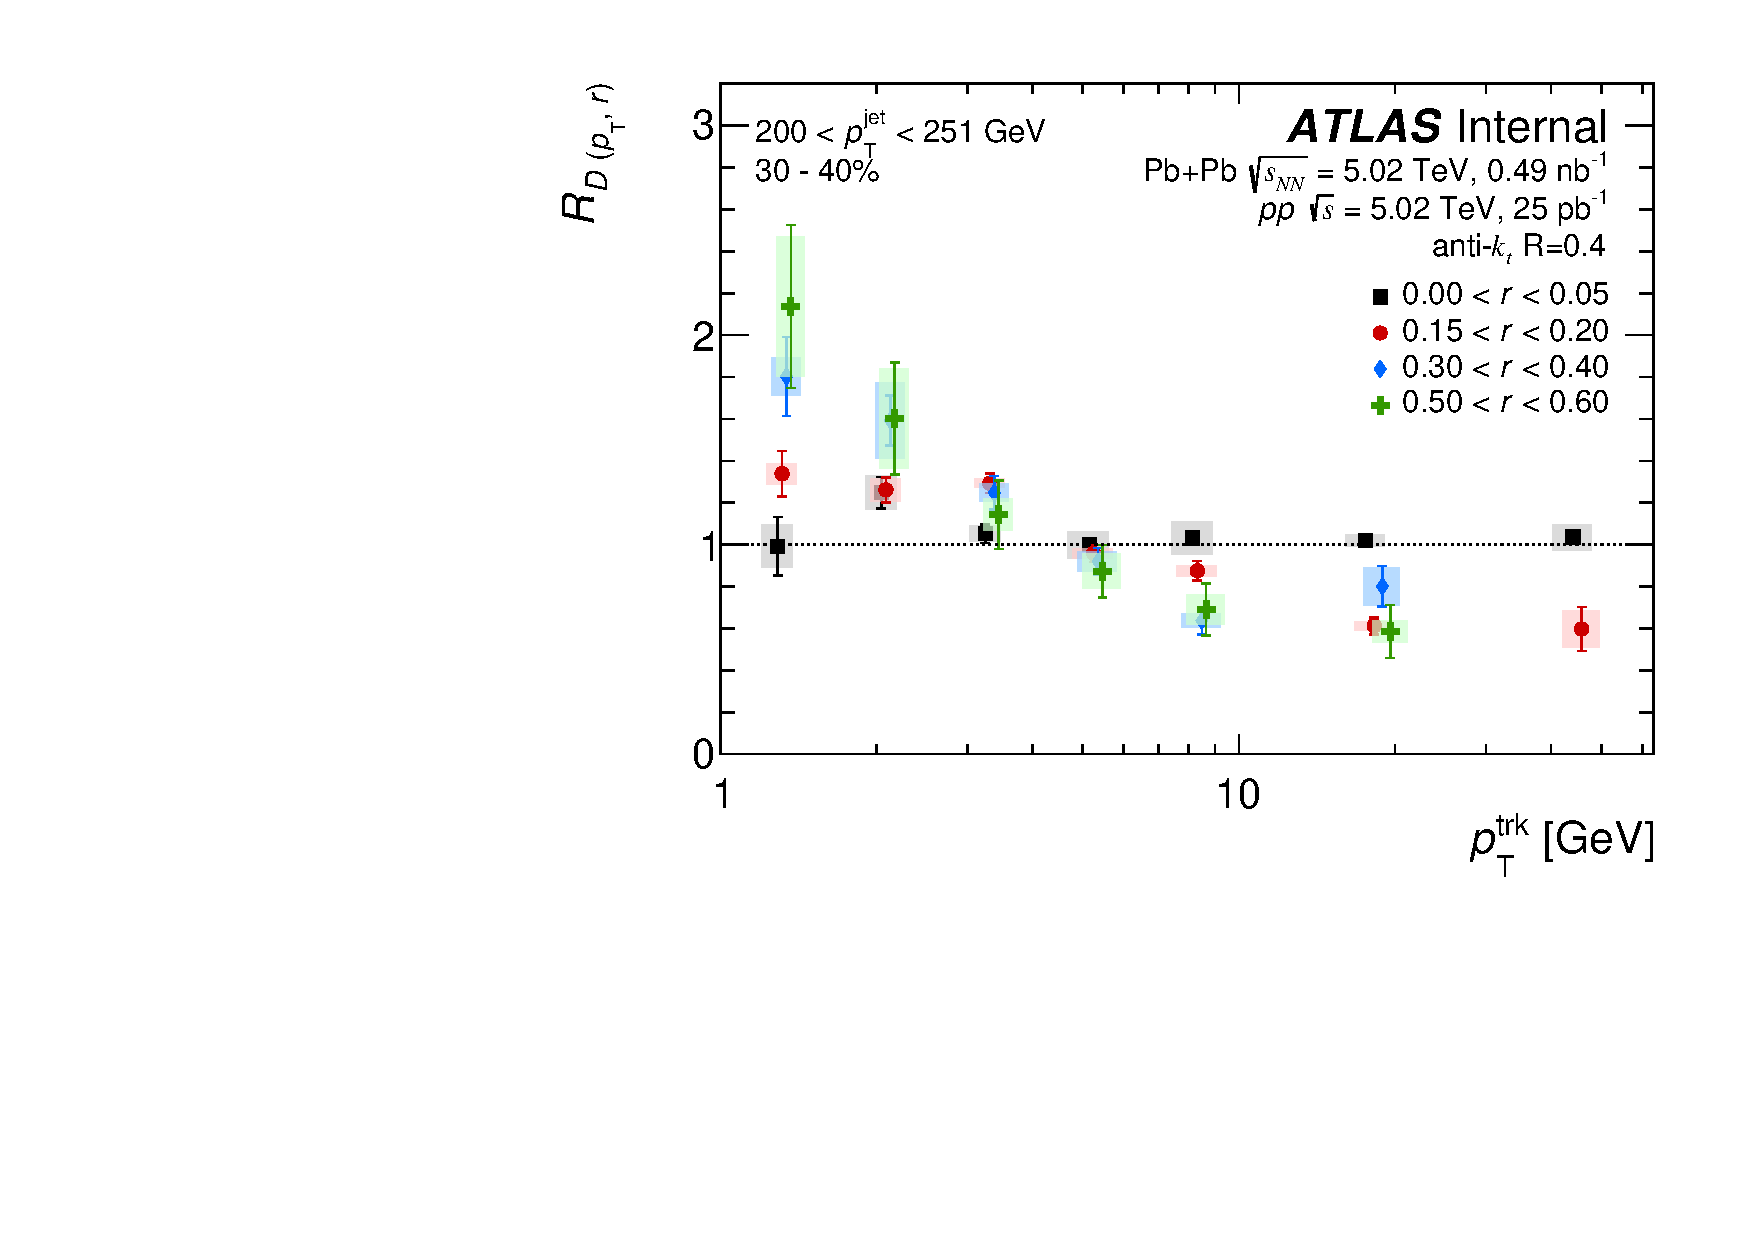
\includegraphics[width=0.5\textwidth]{results/RDpT_trkpt_jet9_cent3} \\
	 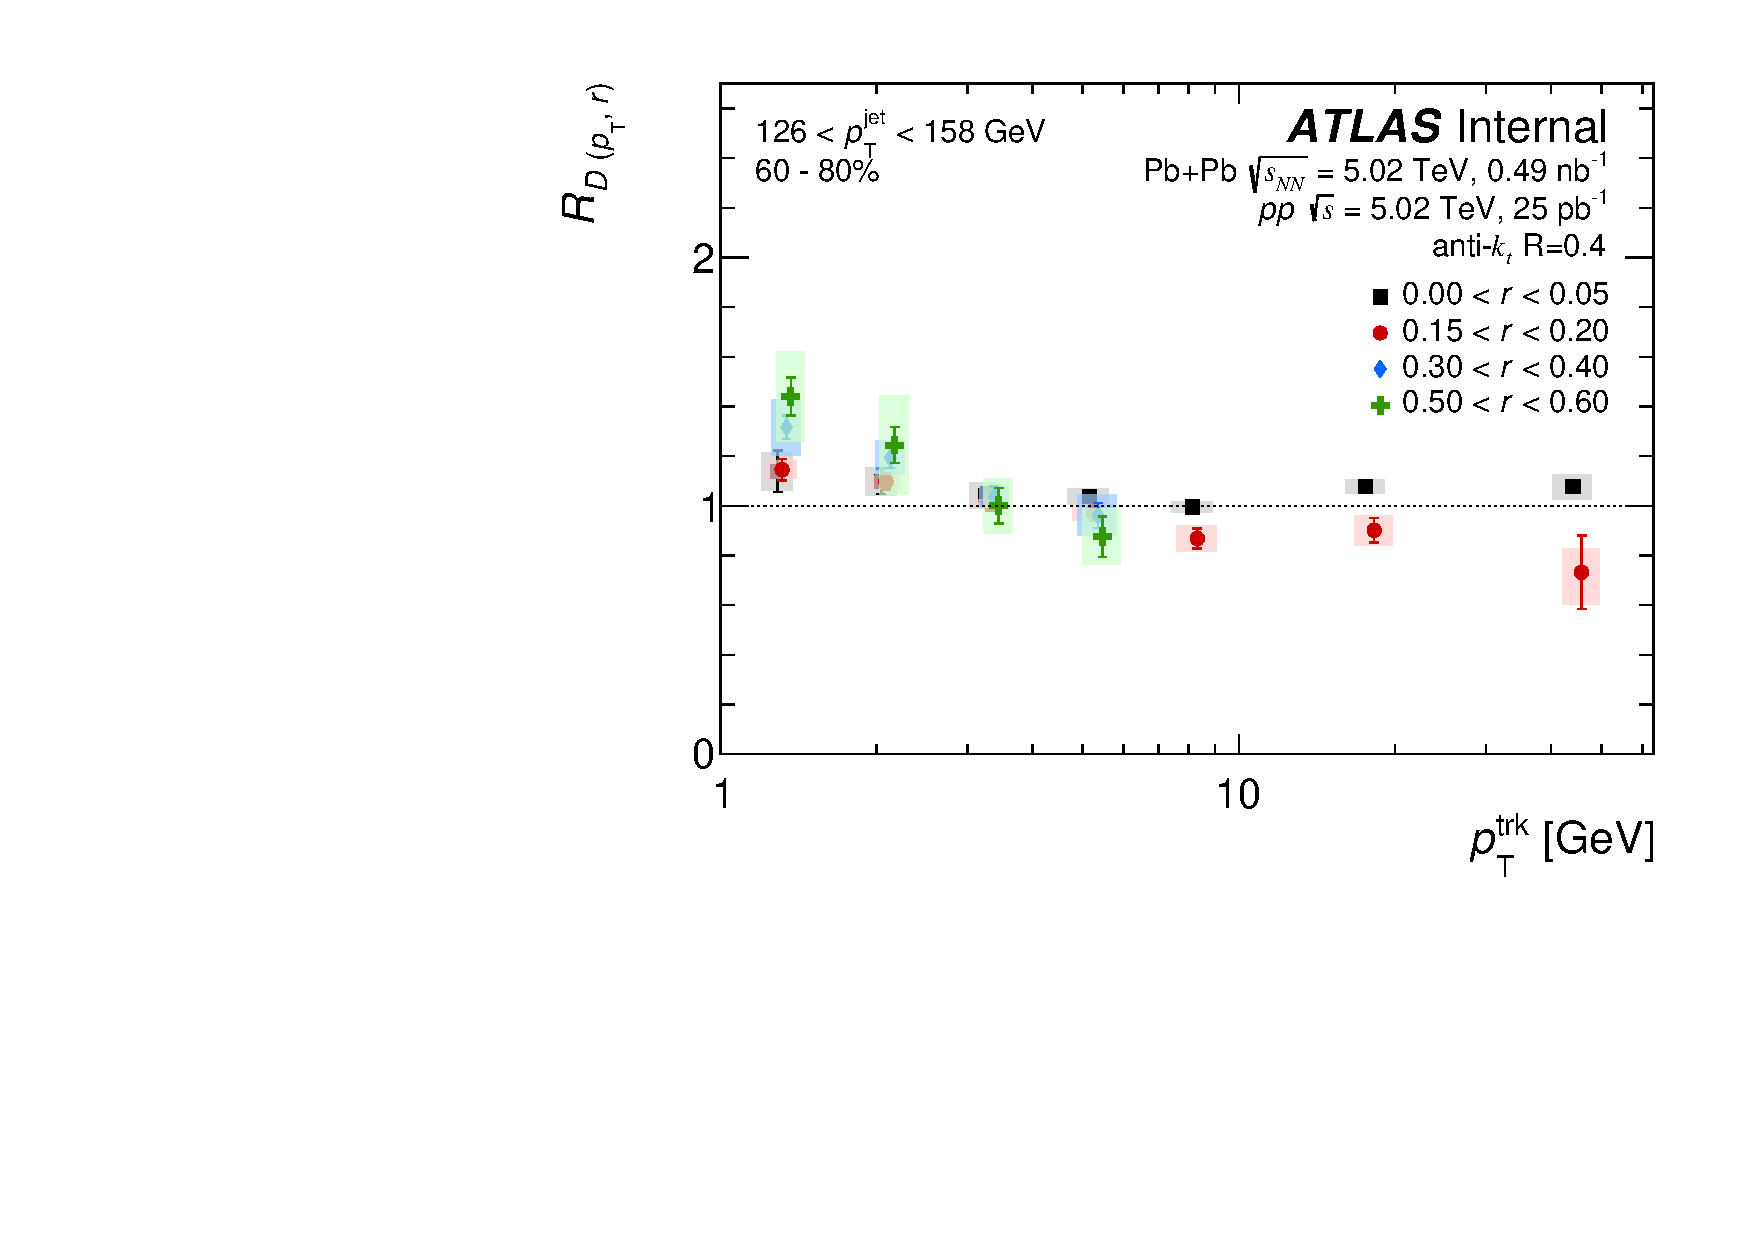
\includegraphics[width=0.5\textwidth]{results/RDpT_trkpt_jet7_cent5} &
	 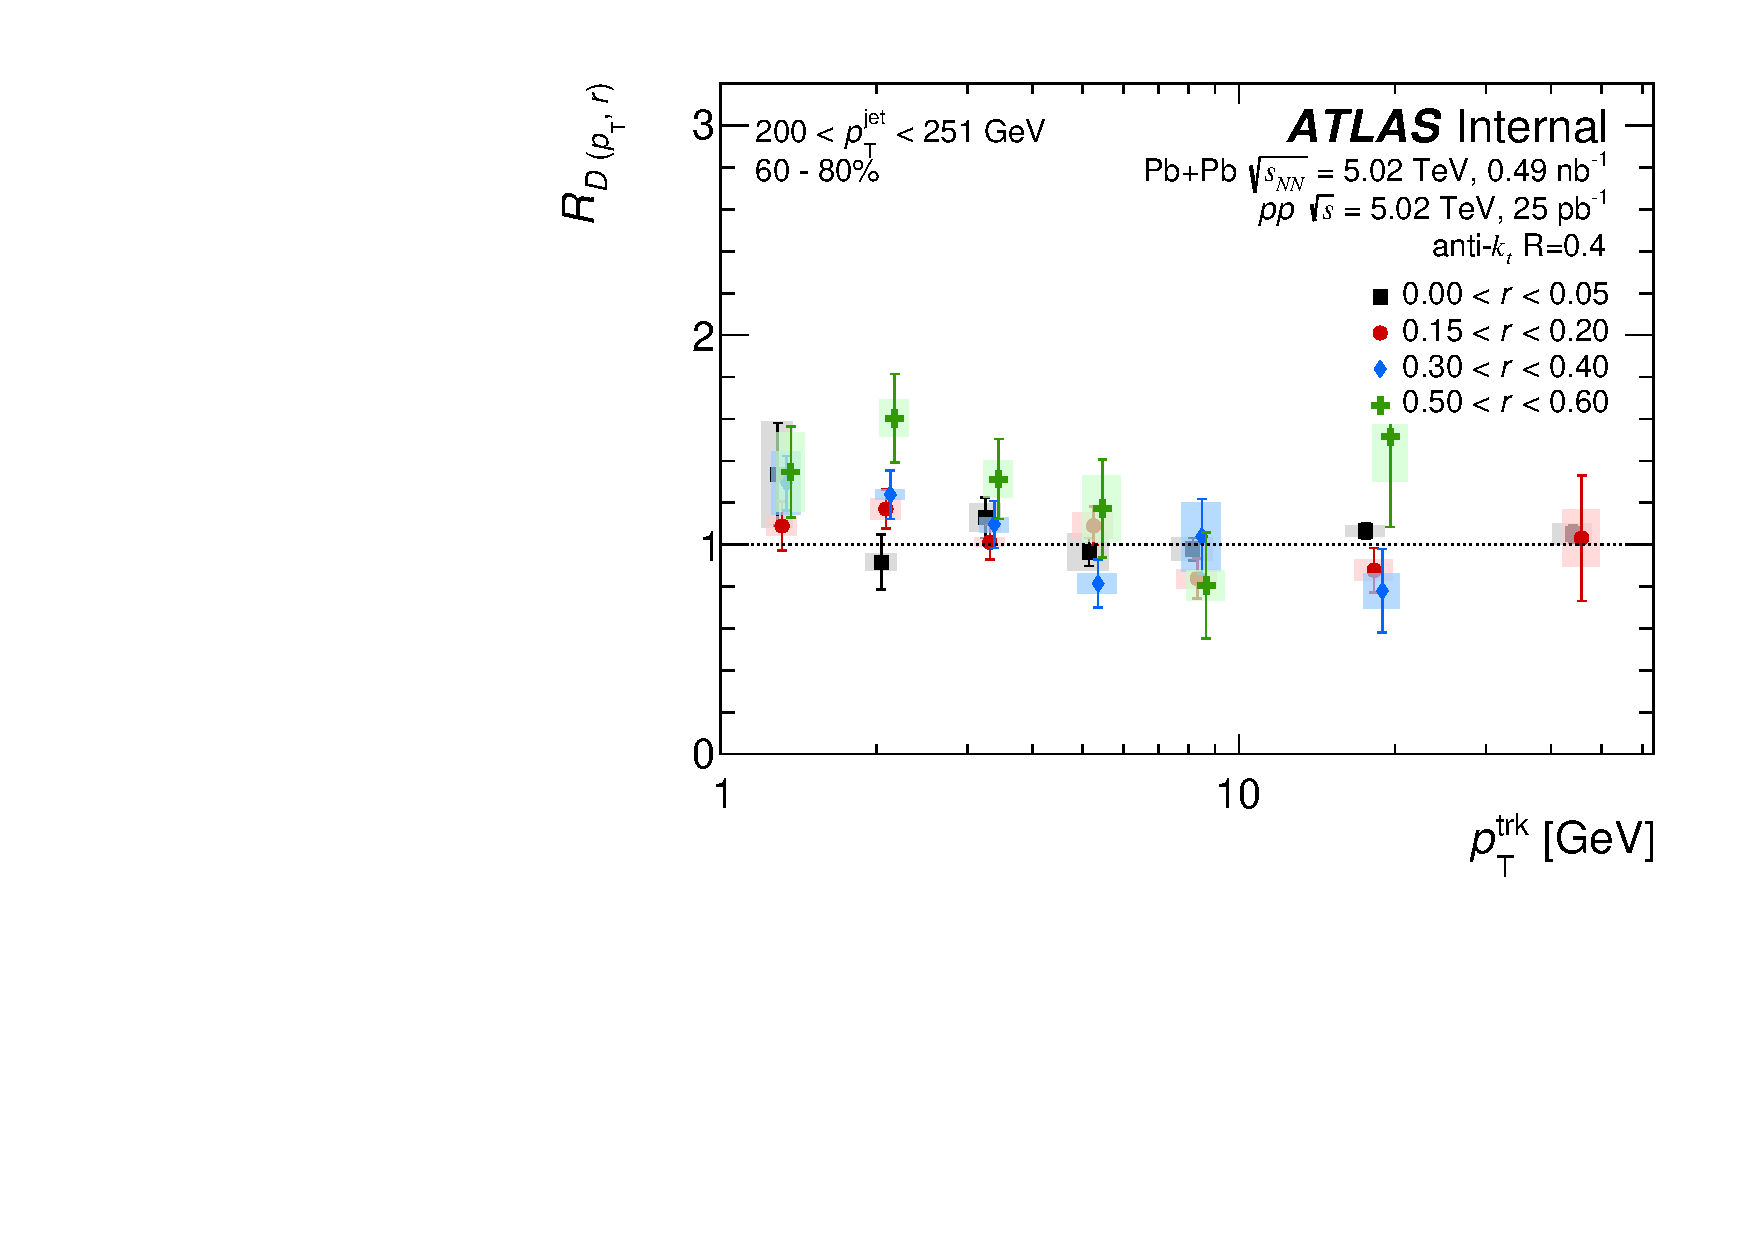
\includegraphics[width=0.5\textwidth]{results/RDpT_trkpt_jet9_cent5} \\
\end{tabular} }
   \caption{\RDptr\ as a function of \pt\ in  0--10\% (top), 30--40\% (middle), and 60--80\% (bottom) \PbPb\ collisions to \pp\ collisions for two different \ptjet\ selections: 126--158~\GeV\ (left) and 200--251~\GeV\ (right). The different colors indicate different angular distances from the jet axis. The vertical bars on the data points indicate statistical uncertainties while the shaded boxes indicate systematic uncertainties. The widths of the boxes are not indicative of the bin size and the points are shifted horizontally for better visibility.}
      \label{fig:pttrkdep}
\end{figure}

\begin{figure}
\centering{
\begin{tabular}{cc}
	 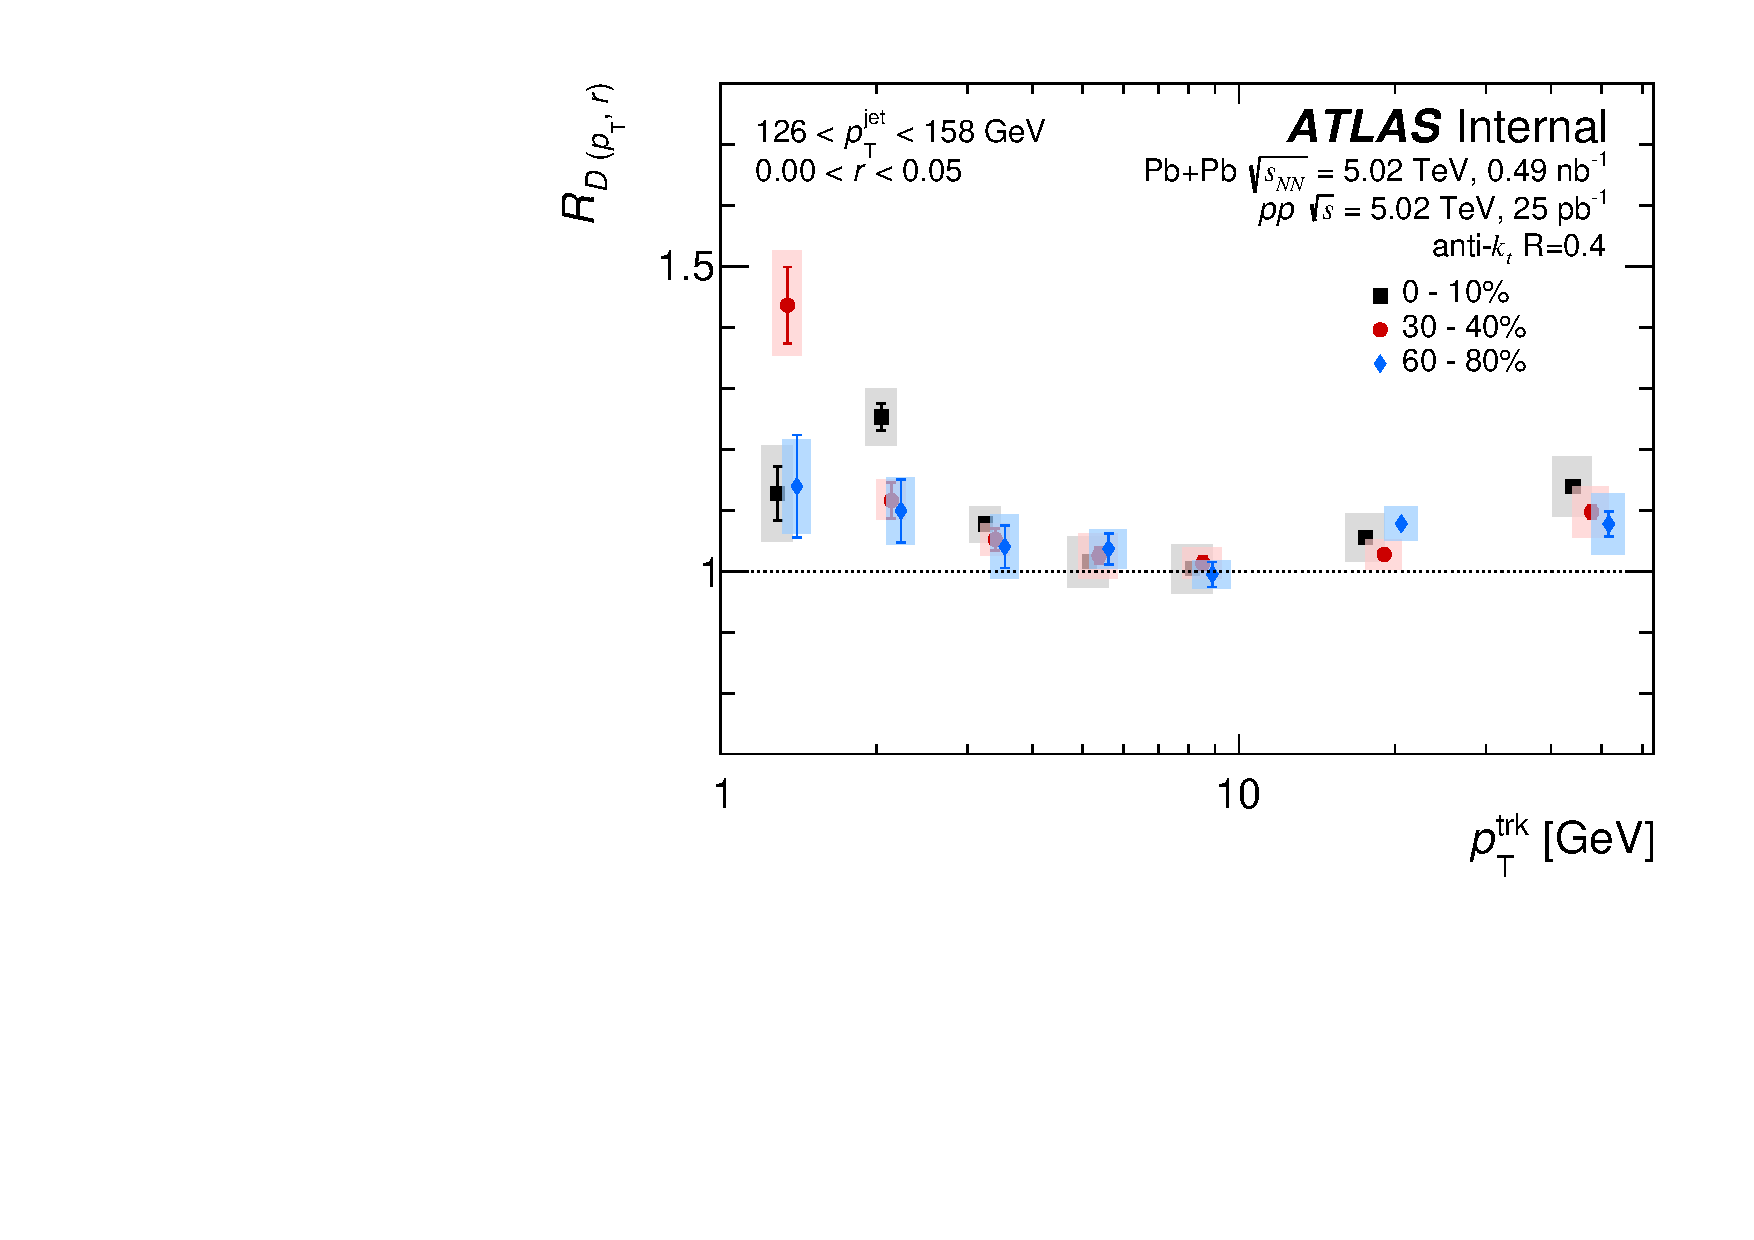
\includegraphics[width=0.5\textwidth]{results/RDpT_trkpt_jet7_dR0} &
	 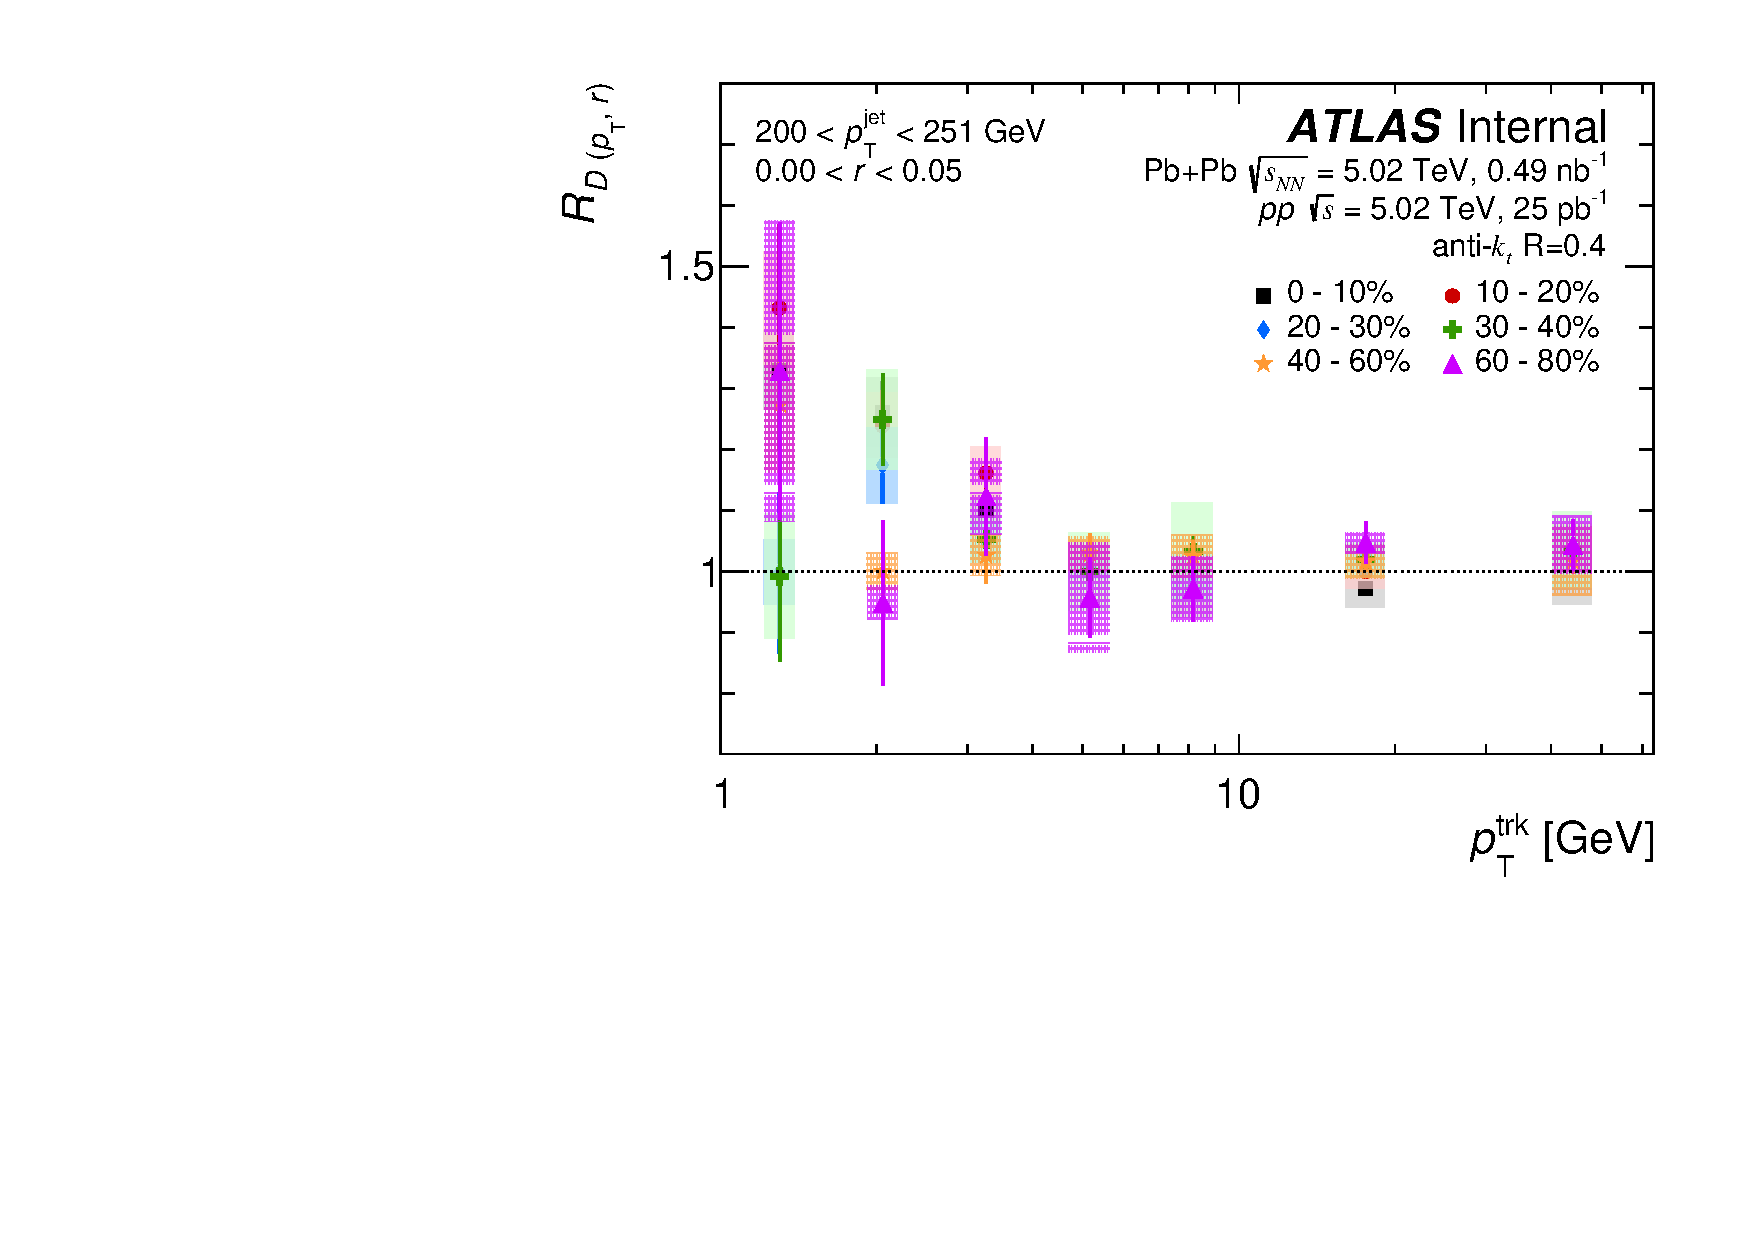
\includegraphics[width=0.5\textwidth]{results/RDpT_trkpt_jet9_dR0} \\
%	 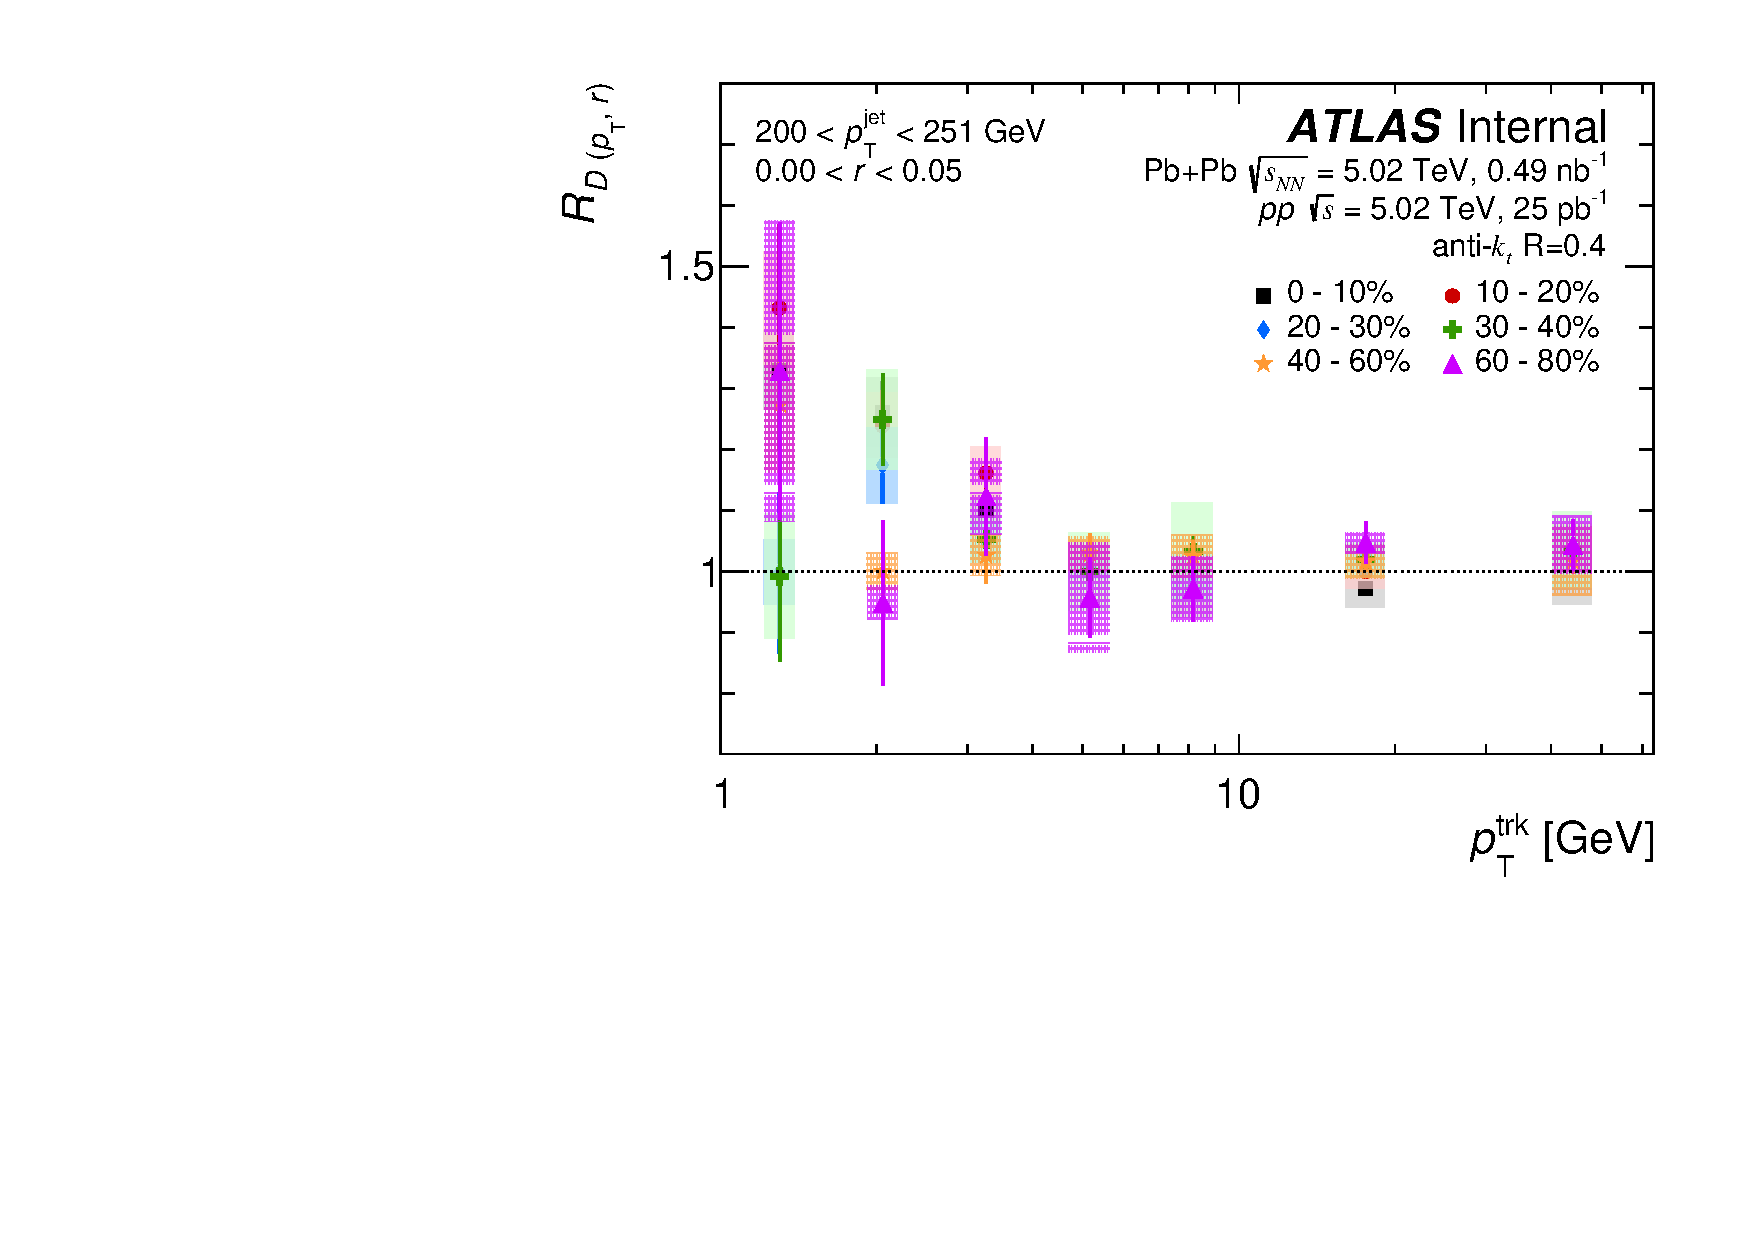
\includegraphics[width=0.5\textwidth]{results/RDpT_trkpt_jet9_dR0} &
%	 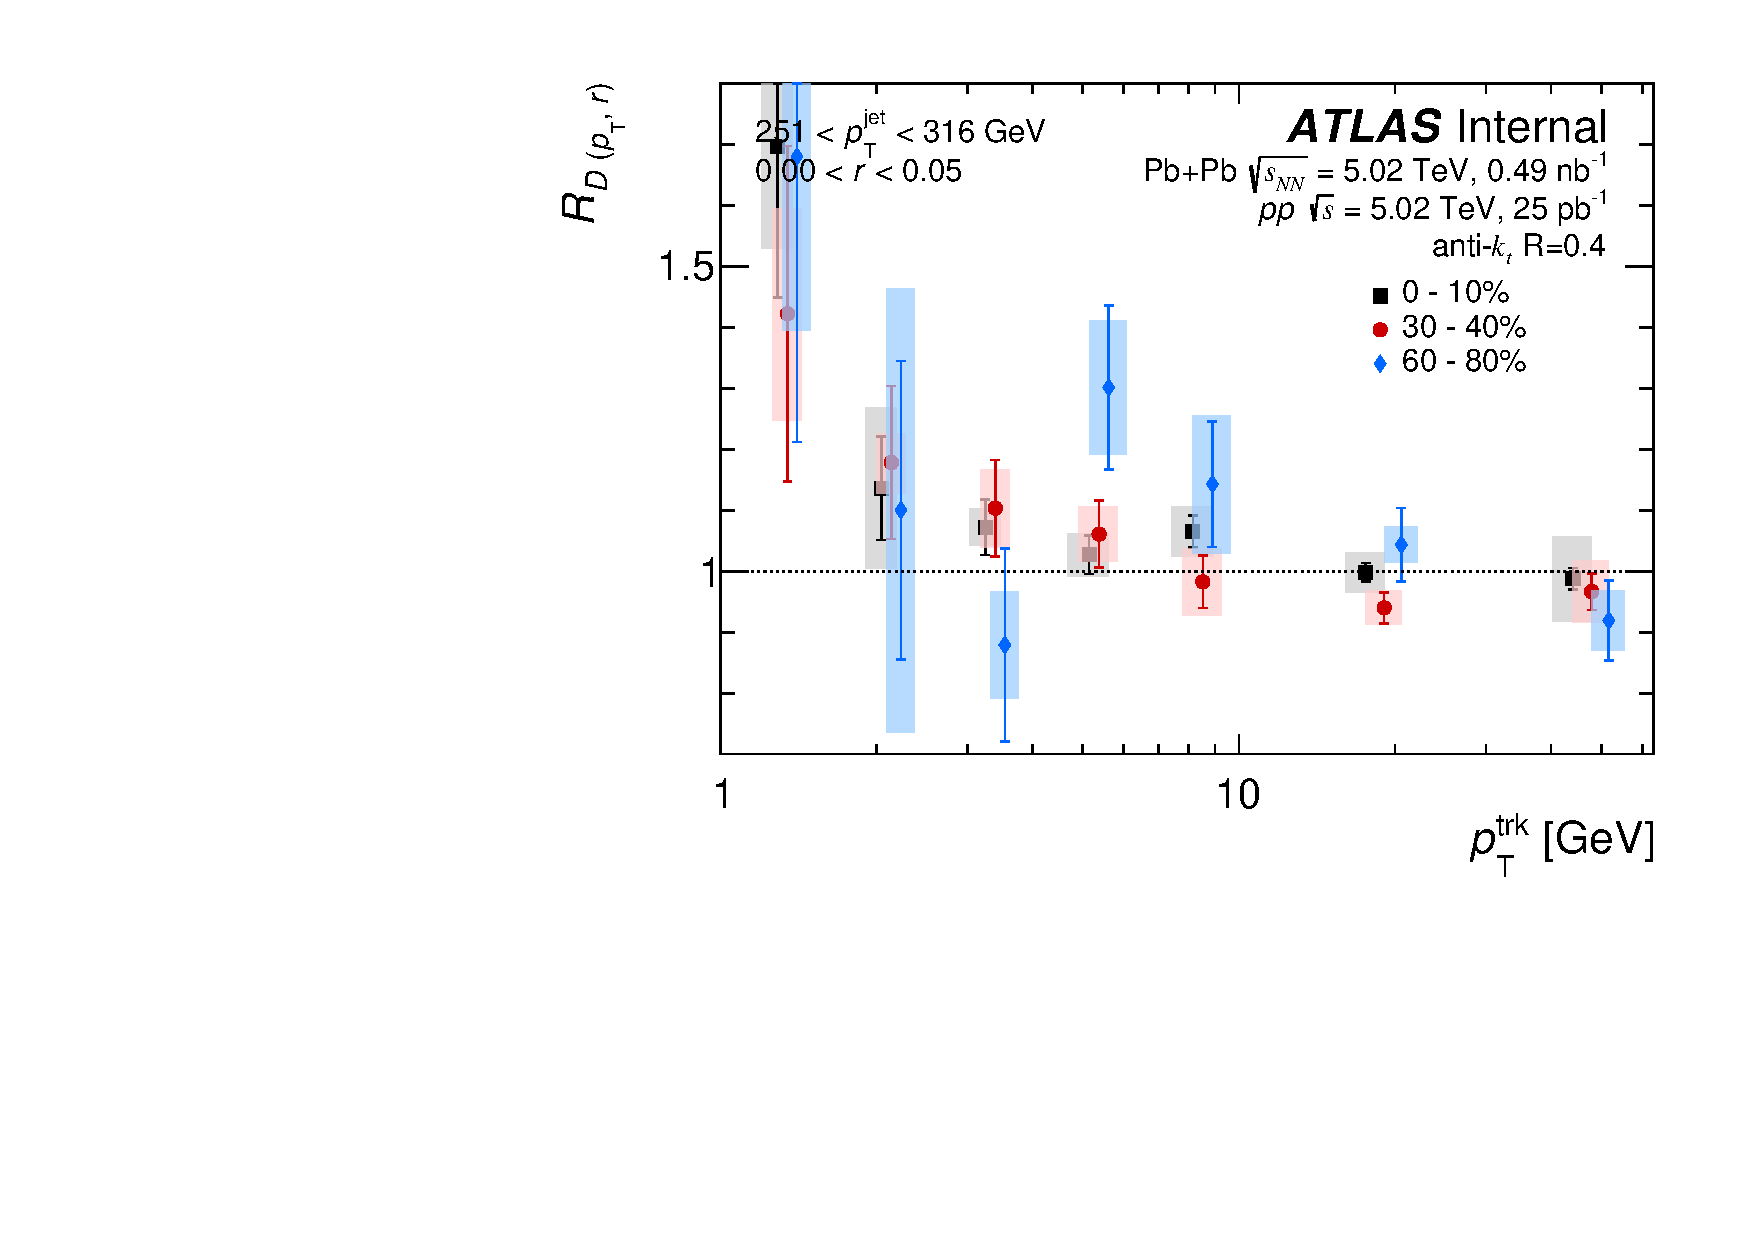
\includegraphics[width=0.5\textwidth]{results/RDpT_trkpt_jet10_dR0} \\
%	 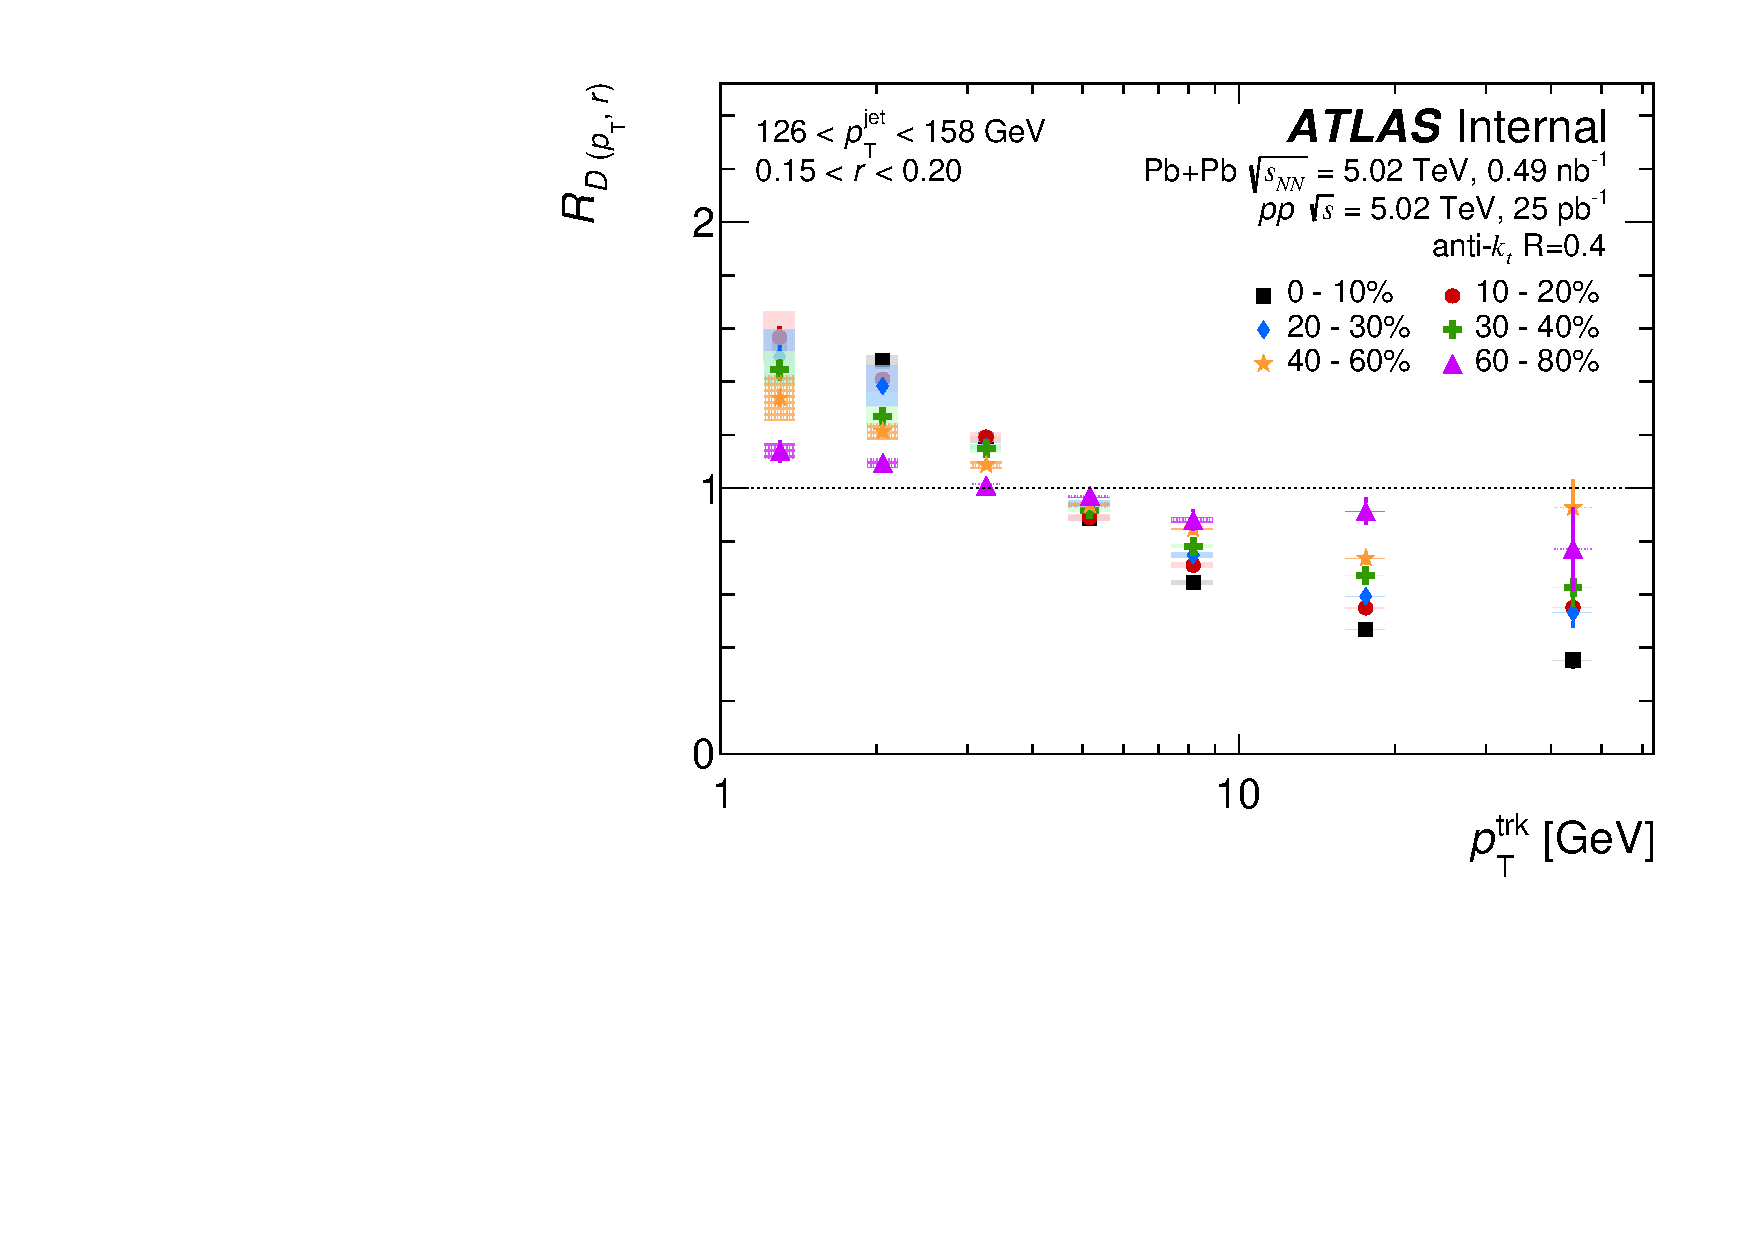
\includegraphics[width=0.5\textwidth]{results/RDpT_trkpt_jet7_dR3} &
%	 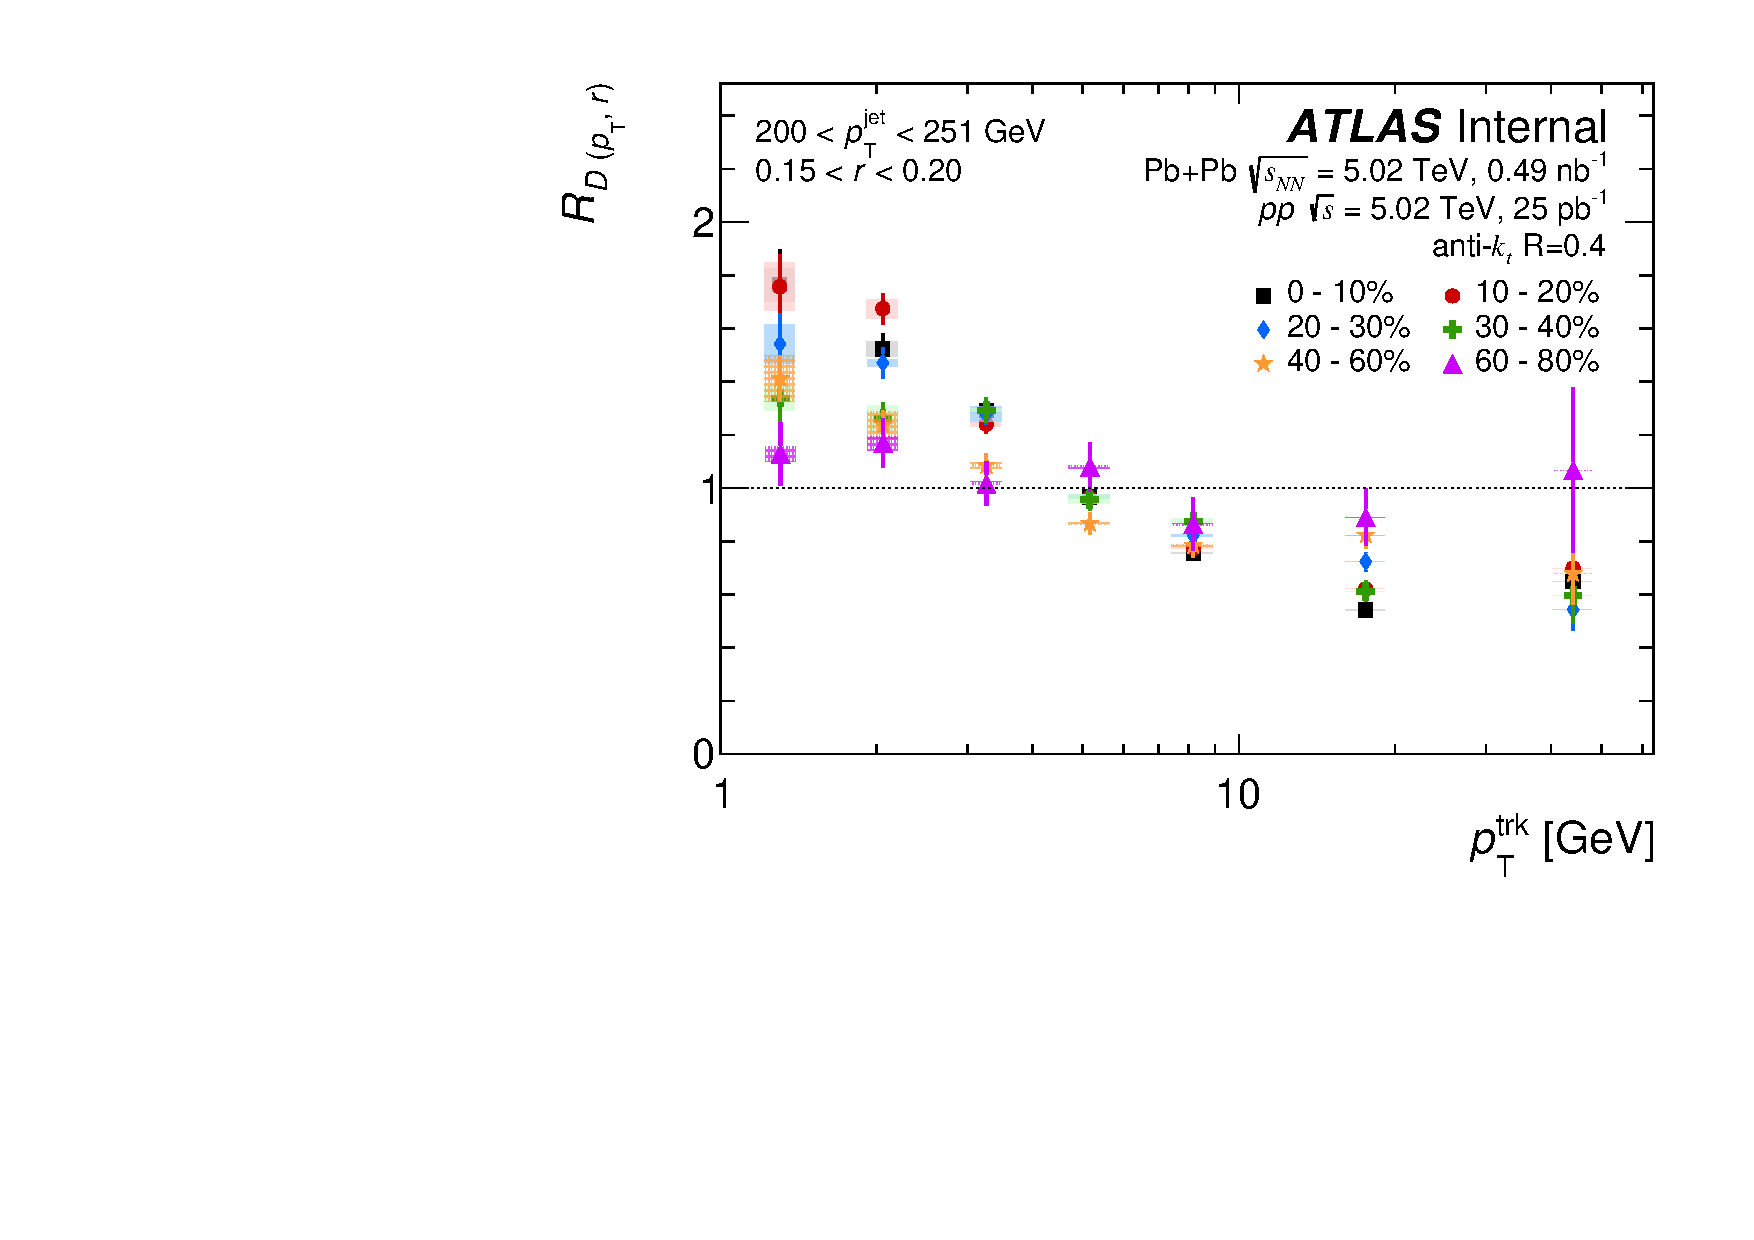
\includegraphics[width=0.5\textwidth]{results/RDpT_trkpt_jet9_dR3} \\
%	 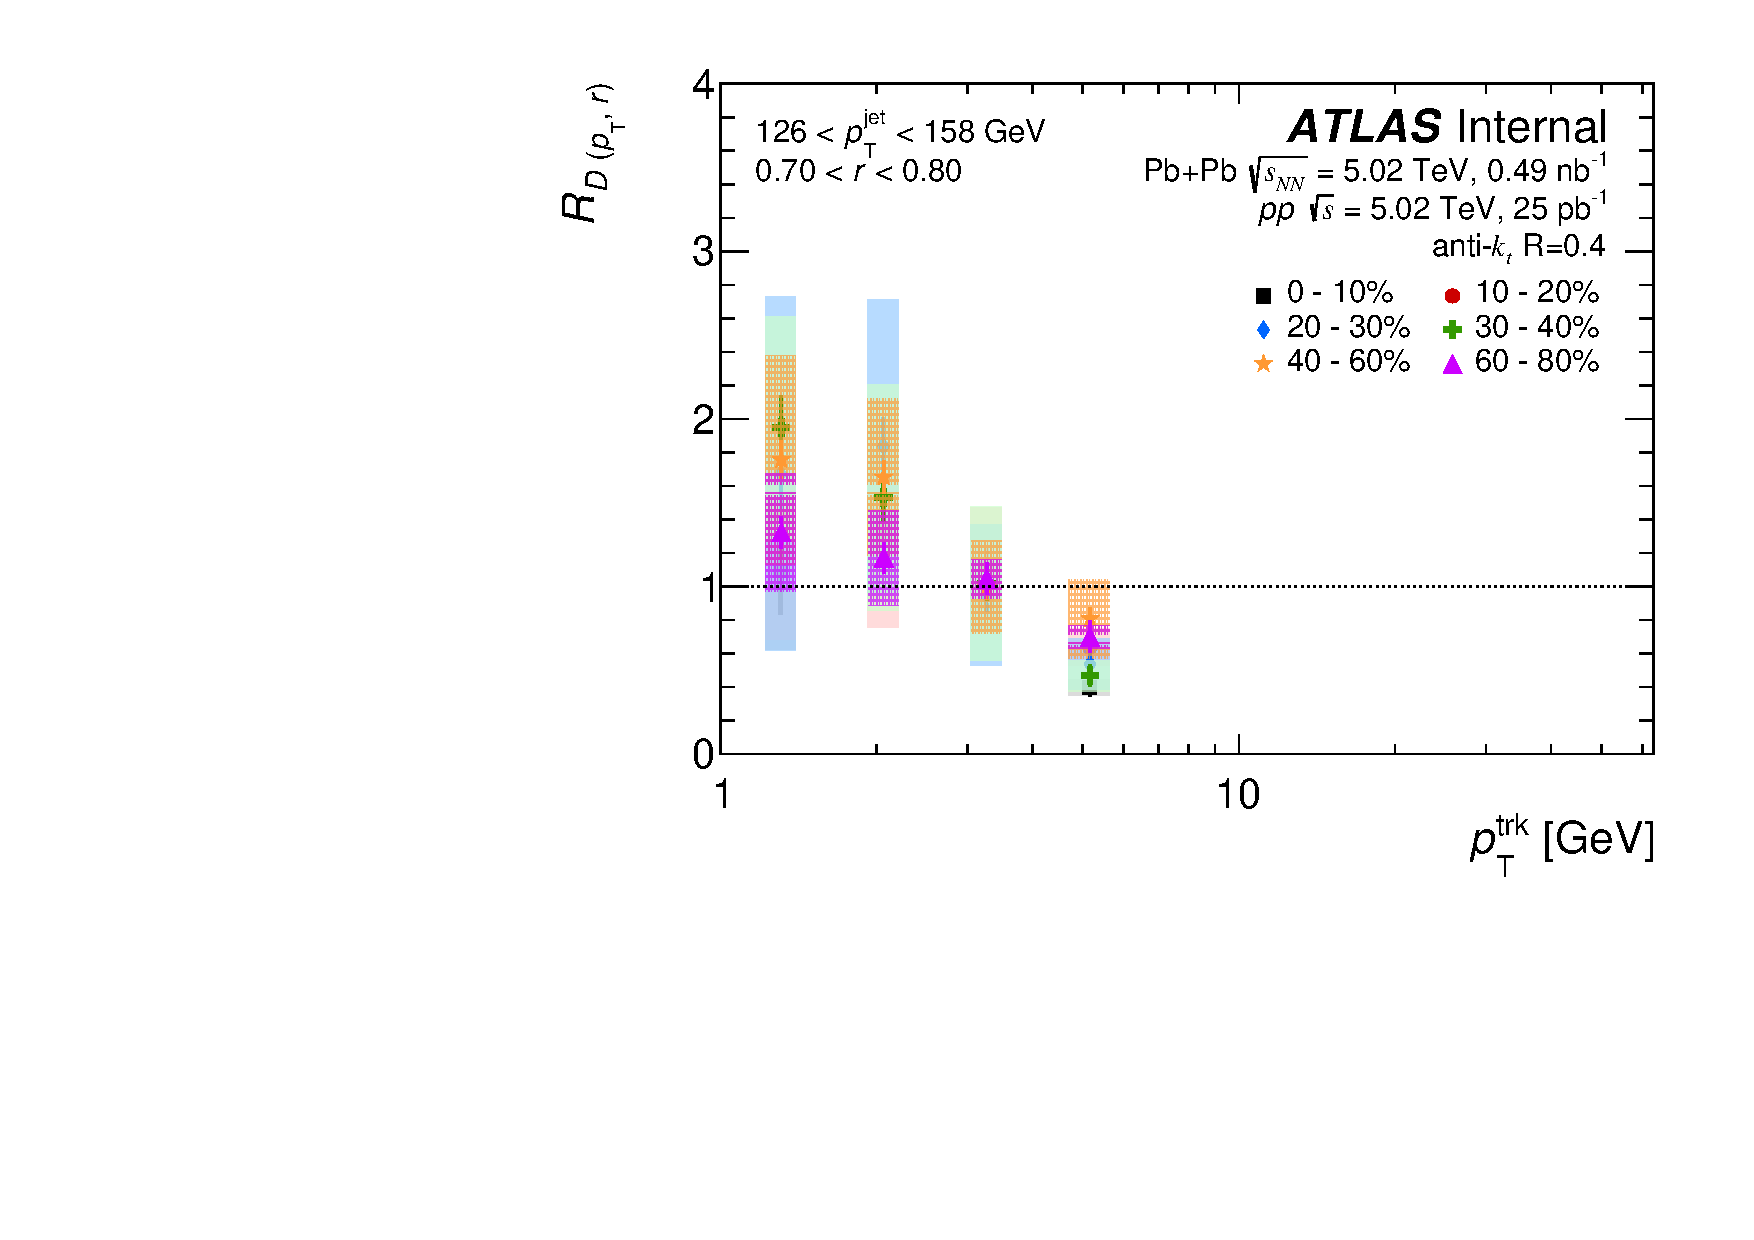
\includegraphics[width=0.5\textwidth]{results/RDpT_trkpt_jet7_dR10} &
%	 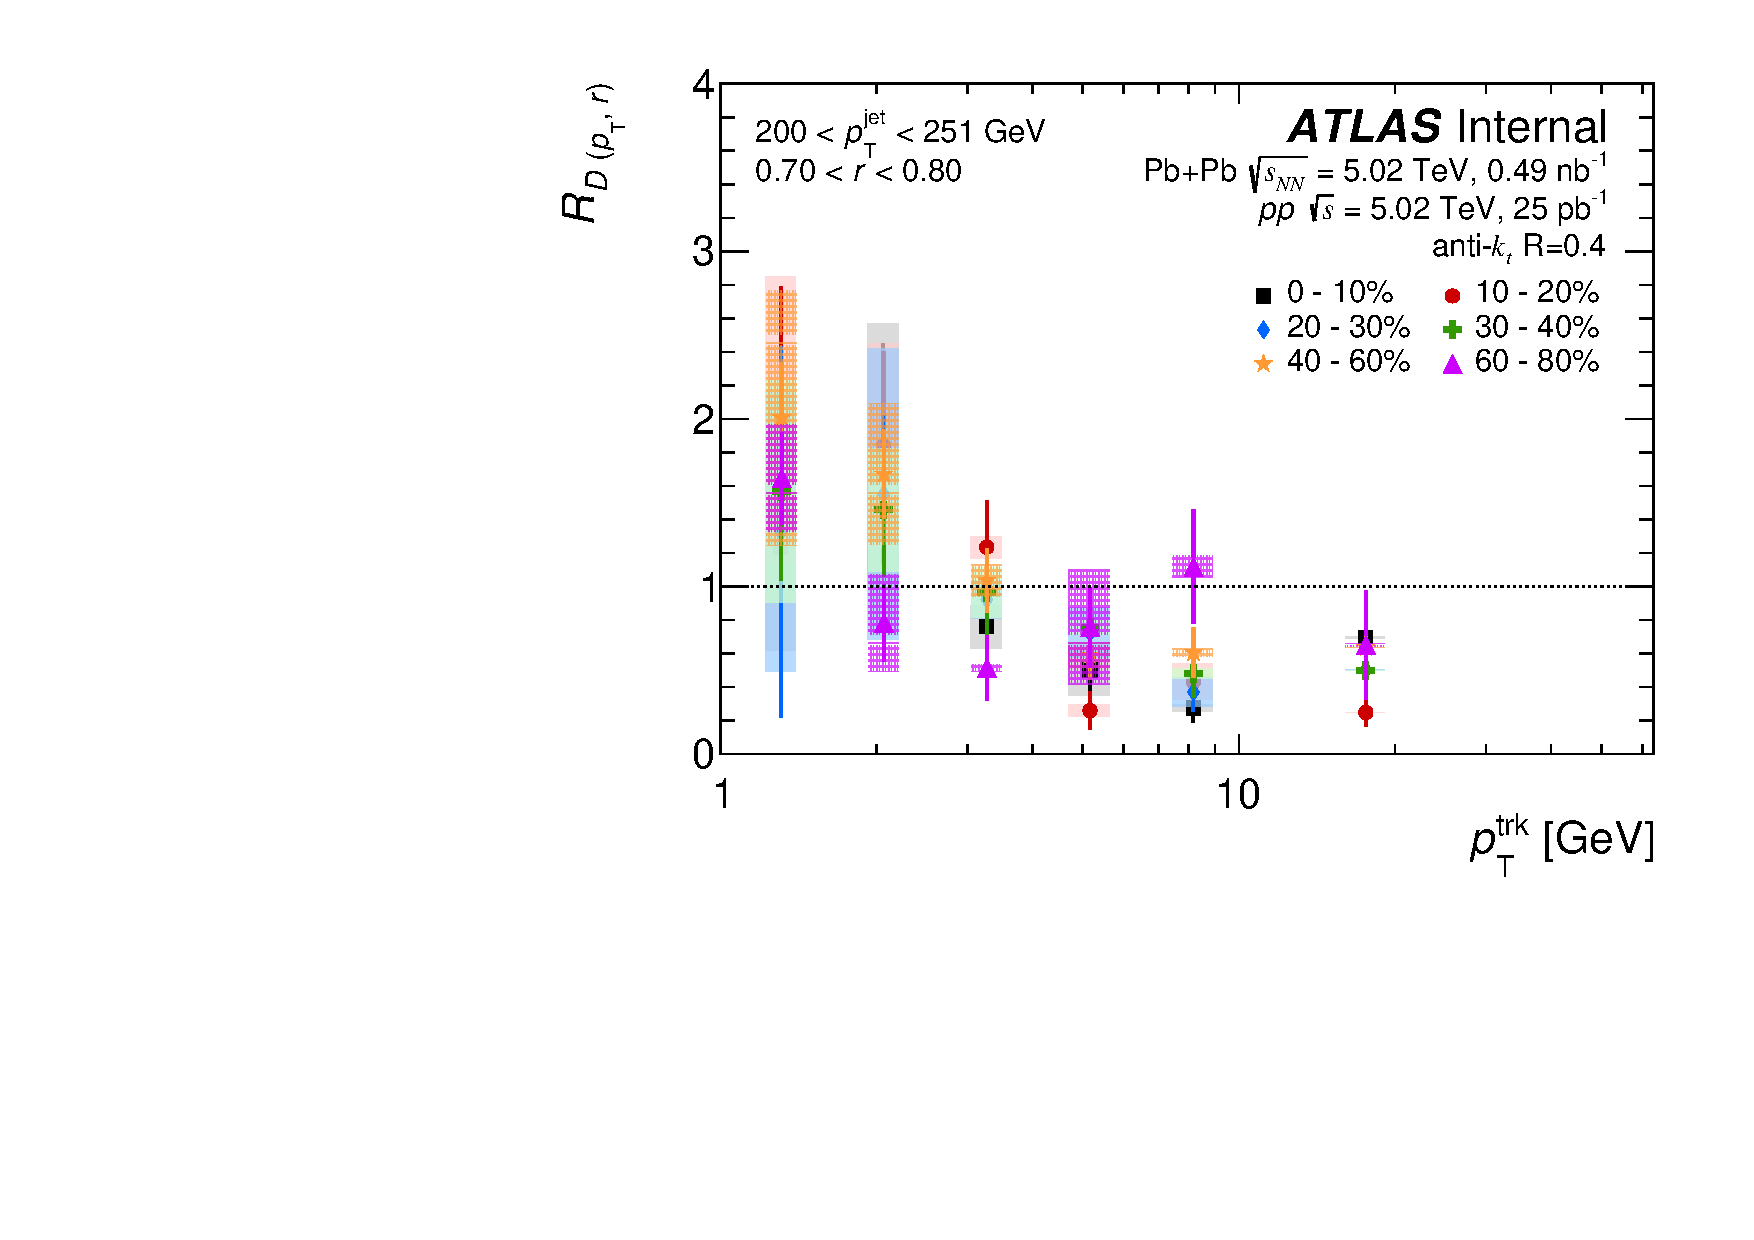
\includegraphics[width=0.5\textwidth]{results/RDpT_trkpt_jet9_dR10} \\
\end{tabular} }
   \caption{\RDptr\ for central \pbpb\ collisions as a function of \pt\ for different jet selections. The different colors represent different centrality bins. The vertical bars on the data points indicate statistical uncertainties while the shaded boxes indicate systematic uncertainties. The widths of the boxes are not indicative of the bin size and the points are shifted horizontally for better visibility.}
      \label{fig:rdptr_trk_cent}
\end{figure}
%%%%%%%%%%%%%




%% DeltaDpT
In addition to the ratios of the \Dptr\ distributions, differences between the charged particle yields were also evaluated to quantify the modification in terms of the particle density. These are given as:

\begin{align}
\DeltaDptr = \Dptr_{\mathrm{Pb+Pb}} - \Dptr_{pp}
\end{align}

These differences are presented as a function of $r$ for different \pt\ selections in 0--10\% central collisions in Figure~\ref{fig:deltadptr}. 
These distributions show an excess  in the charged-particle yield density for \pbpb\ collisions compared to \pp\ collisions for charged particles with $\pt <4.0$ GeV. This excess ranges from 0.5 to 4 particles per unit area at 1 \GeV\ in 126--158~\GeV\ jets for 0--10\% central \pbpb\ collisions and increases with increasing \ptjet. 
The largest excesses for charged particles with $\pt <$~4.0~\GeV\ is within the jet cone.  For large \rvar\ values, the
density decreases, but remains positive.
A depletion for higher \pt\ particles is at most 0.5 particles per unit area for 126--158~\GeV\ jets in 0--10\% central \pbpb\ collisions that increases for higher \ptjet. 
One possible explanation of the modification of the 
jet fragmentation in this kinematic range~\cite{Aaboud:2018hpb} is the larger expected energy loss
of gluon-initiated jets leading to a relative enhancement of quark jets in \pbpb\ collisions compared
to \pp\ collisions at a given \ptjet\ value~\cite{Spousta:2015fca}. Since gluon jets have a broader distribution of particle transverse momentum with respect to the jet direction compared to quark-initiated jets \cite{OPAL:1995ab}
 , such an effect could potentially describe the narrowing of particle distribution around the jet direction for particles with $\pt >$~4.0~\GeV\
observed here, though no calculations of this are available.
%For particles with 25.1~$< \pt <$~63.1~\GeV, the \DeltaDptr\ distribution is consistent with unity over the entire measured range of \rvar\ and \ptjet.
There is a minimum in the \DeltaDptr\ distribution for charged particles with \mbox{$ 4.0 < \pt <  25.1$}~\GeV\ at $0.05 < \rvar < 0.10$ that is seen at all \ptjet\ ranges under investigation.

\begin{figure}
\centering{
\begin{tabular}{cc}
	 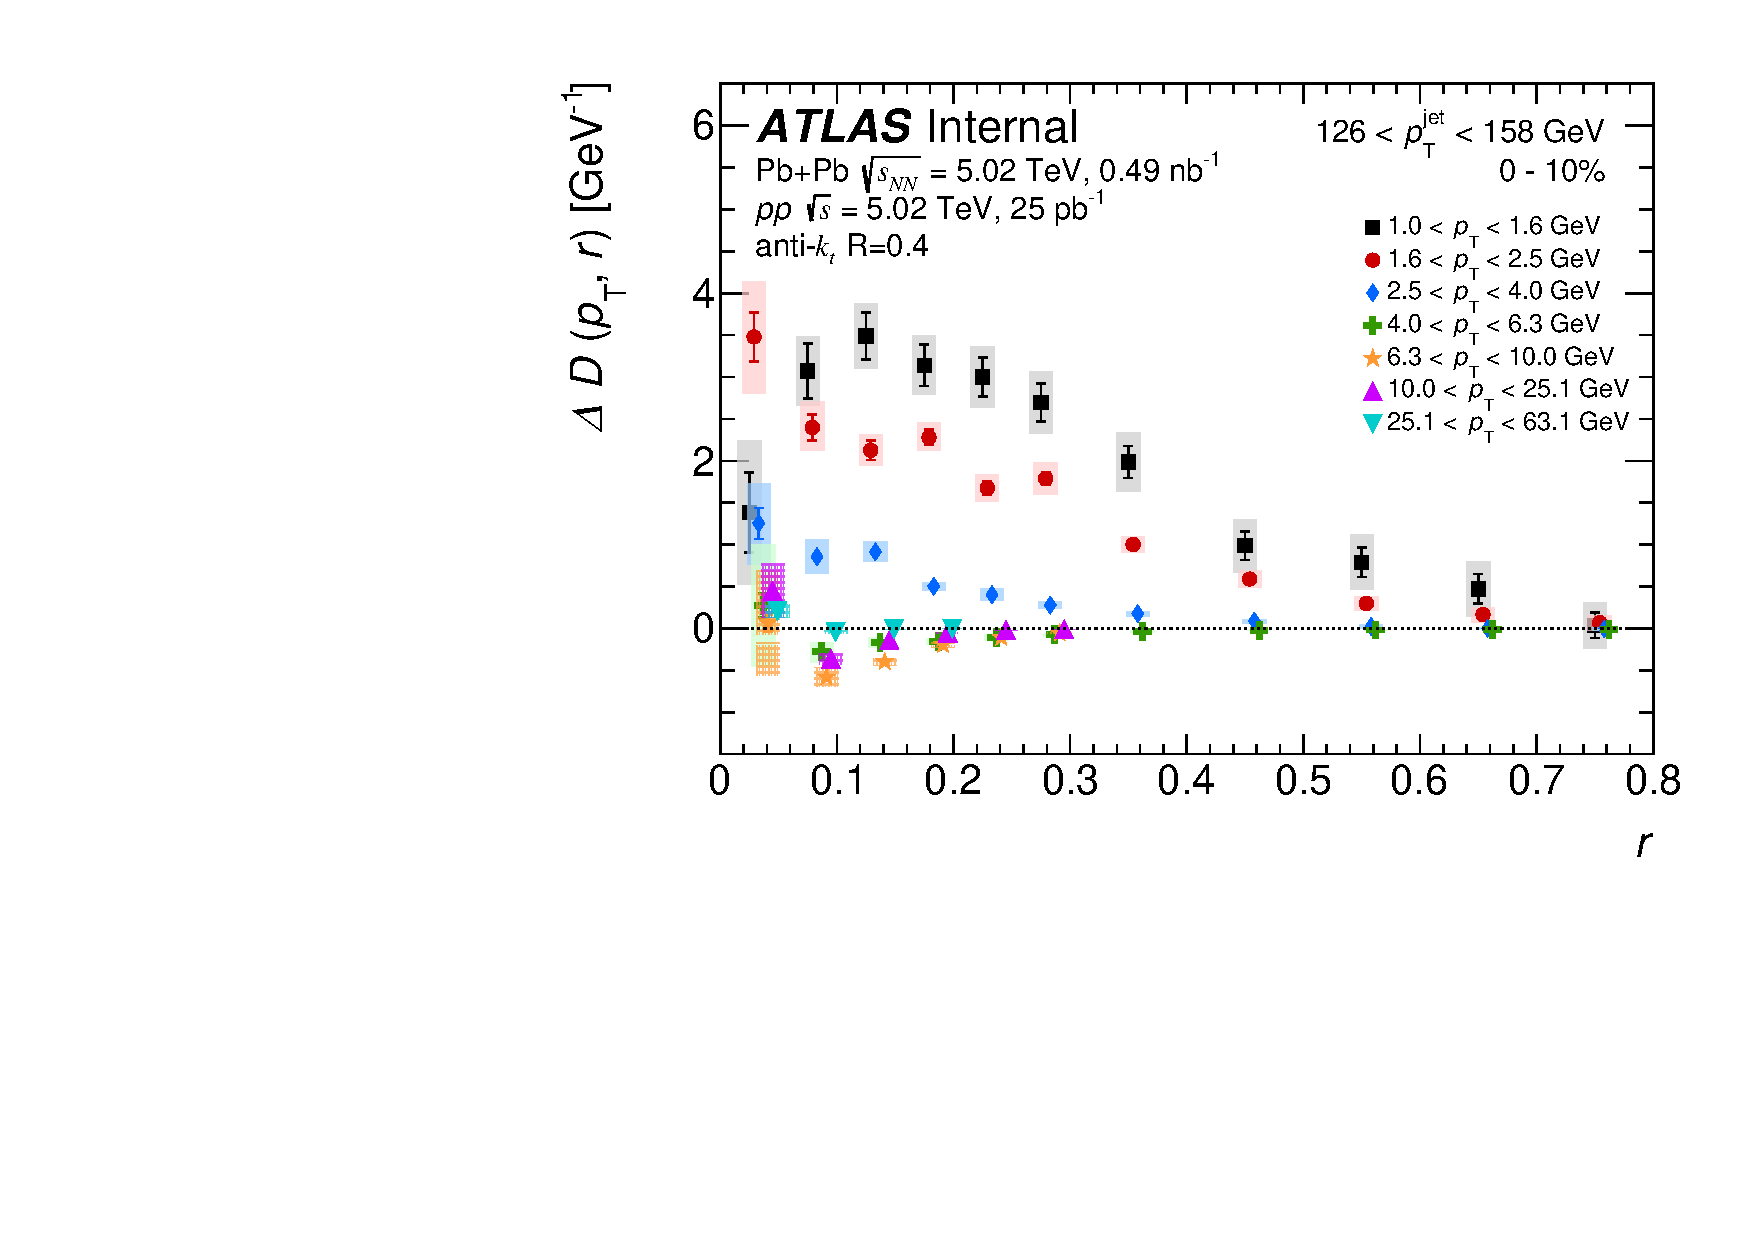
\includegraphics[width=0.5\textwidth]{results/DeltaDpT_dR_jet7_cent0} &
	 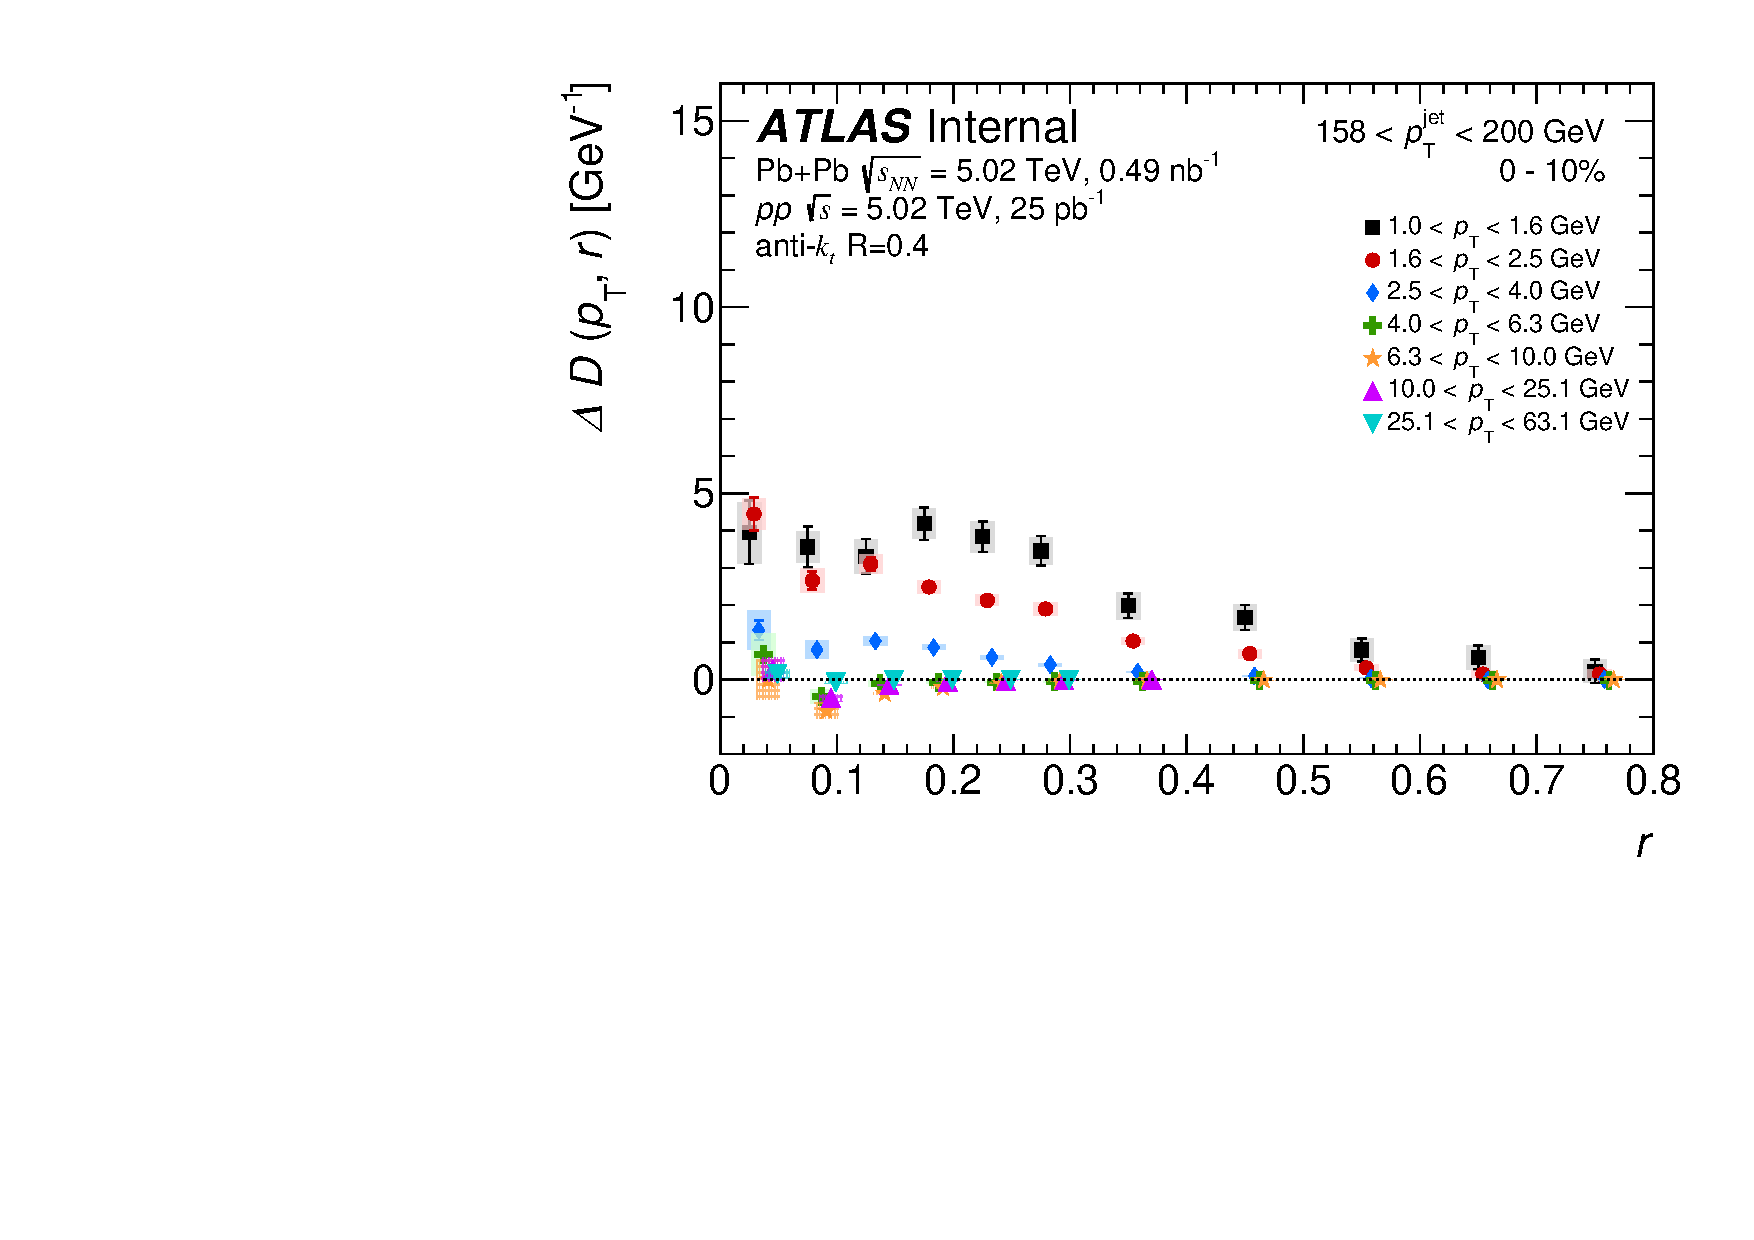
\includegraphics[width=0.5\textwidth]{results/DeltaDpT_dR_jet8_cent0} \\
	 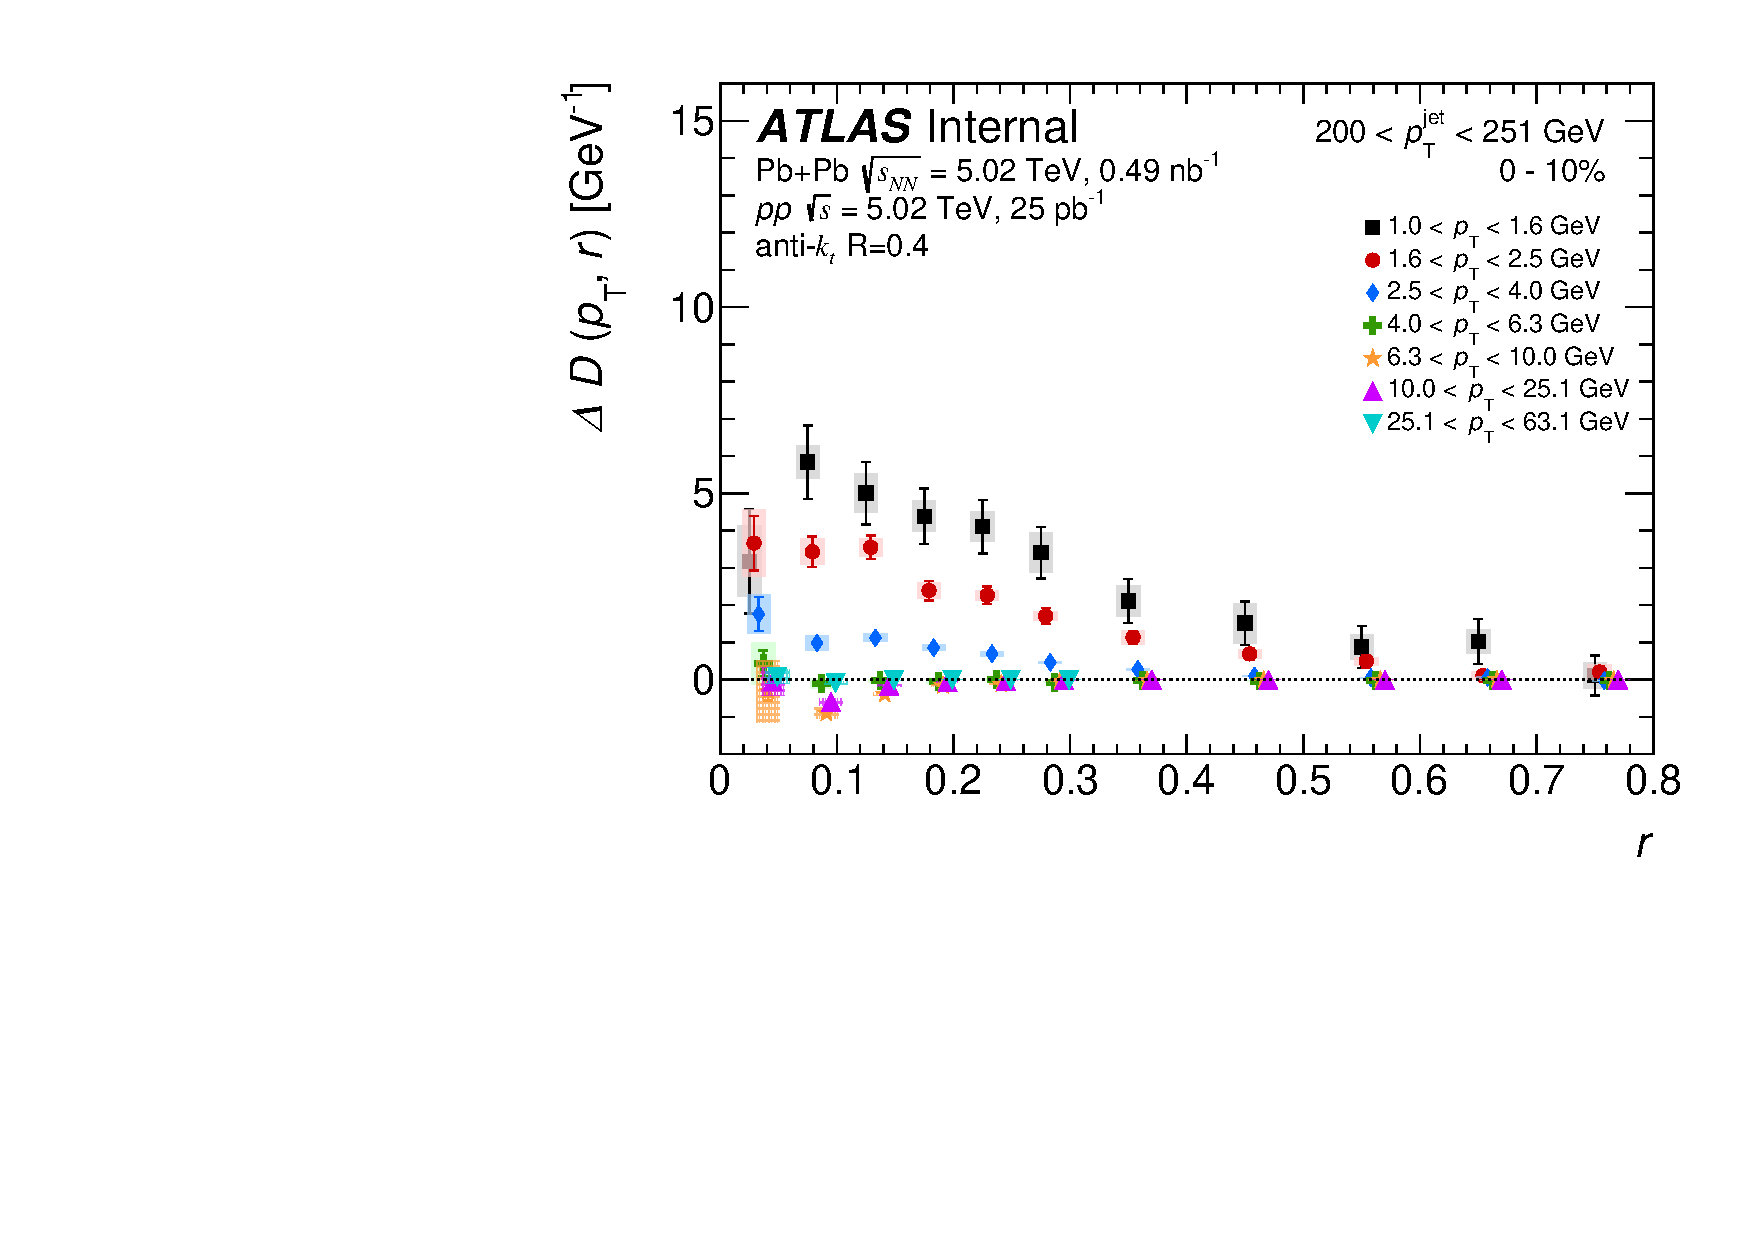
\includegraphics[width=0.5\textwidth]{results/DeltaDpT_dR_jet9_cent0} &
	 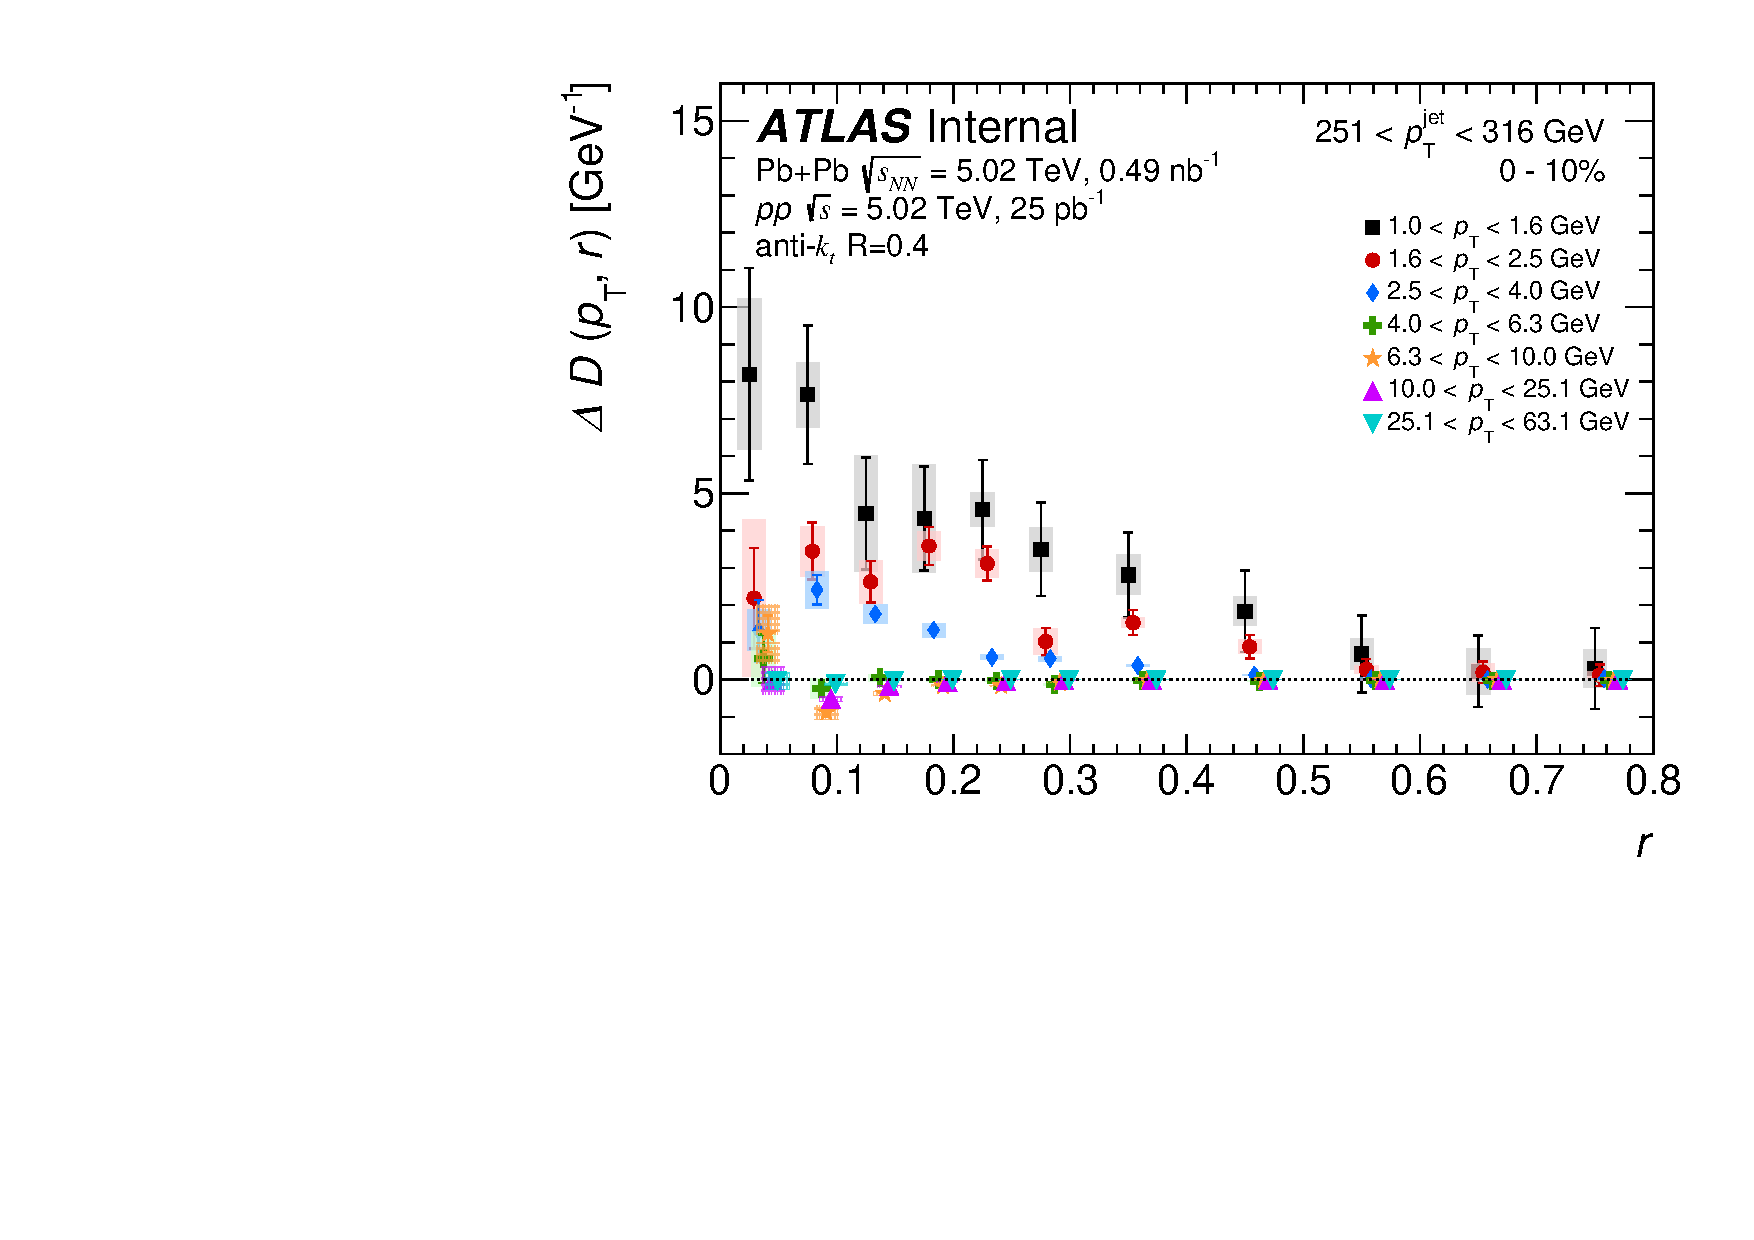
\includegraphics[width=0.5\textwidth]{results/DeltaDpT_dR_jet10_cent0} \\
\end{tabular} }
   \caption{\DeltaDptr\ as a function of \rvar\ in central collisions for all \pt\ ranges in four \ptjet\ selections: 126--158~\GeV, 158--200~\GeV, 200--251~\GeV, and 251--316~\GeV. The vertical bars on the data points indicate statistical uncertainties while the shaded boxes indicate systematic uncertainties. The widths of the boxes are not indicative of the bin size and the points are shifted horizontally for better visibility. }
      \label{fig:deltadptr}
\end{figure}
%%%%%%%%%%%%%

%\subparagraph{Integrated plots}
Motivated by similar studies of the enhancement of soft fragments with $\pt < 4.2$ GeV in jet fragmentation functions in \pbpb\ compared to \pp\ collisions from \cite{PhysRevC.98.024908}, the \Dptr\ distributions can be integrated for charged particles with \pt\ < 4 GeV to construct the quantities $\Theta$ and $P$ given as:

\begin{align}
   \Theta(\rvar) &= \int_1^{4} \Dptr  \fd \pt \\
   P(\rvar) &= \int_0^r \int_1^{4} \Dptr \fd \pt \fd r'
\end{align}

These can be compared between the \pp\ and \pbpb\ systems to give the following distributions:

\begin{align}
 \Delta_\Theta(\rvar) = \Theta(\rvar)_{\mathrm{Pb+Pb}} - \Theta(\rvar)_{pp} & \qquad \Delta_P(\rvar) = P(\rvar)_{\mathrm{Pb+Pb}} - P(\rvar)_{pp} \\
   R_\Theta(\rvar) = \frac{\Theta(\rvar){\mathrm{Pb+Pb}}}{\Theta(\rvar)_{\mathrm{pp}}} &  \qquad R_{P(\rvar)} = \frac{P(\rvar)_{\mathrm{Pb+Pb}}}{P(\rvar)_{pp}}
\end{align}

These variables provide aggregate information for particles with \pt < 4 GeV, both differentially ($\Theta$ quantities)
and cumulatively ($P$ quantities) in \rvar.
Figure~\ref{fig:deltaPdeltaT} shows the \DeltaTheta\ and \DeltaP\ distributions as a function of \rvar. 
The \DeltaTheta\ distributions provide similar information to the \DeltaDptr\ distributions shown in Figure~\ref{fig:deltadptr},
now integrated for $\pt <$~4.0~\GeV.  
A significant \ptjet\ dependence to the enhancement of the soft jet fragments as well as low \pt\ particles outside the jet cone per unit area is observed.
The size of the \ptjet\ dependence to the enhancement is reduced with decreasing collision centrality and is not statistically significant in peripheral collisions.

%Now, the \ptjet\ dependence to the excess in charged-particle density can be seen clearly; 
%in the most central collisions
%there is an increase in \DeltaTheta\ with increasing \ptjet, but in the mid-central and peripheral collisions this is no longer
%observed within the uncertainties.

Moreover, the \DeltaP\ distribution shows that there is an extra particle density of 0.5 when integrated up to $\rvar = 0.8$ around the jet cone. 
The ratios \RTheta\ and \RP\  are shown in 
figure~\ref{fig:RPRT} for the same collision centralities and \ptjet\ ranges. It can be seen that the size of the enhancement is approximately constant for $r > 0.5$.

%\begin{align}
%\Delta_\Theta = \int_1^{4} \Dpt_{\mathrm{PbPb}} - \Dpt_{\mathrm{pp}} \fd \pt
%\end{align}
\begin{figure}
\centering{
\begin{tabular}{cc}
	 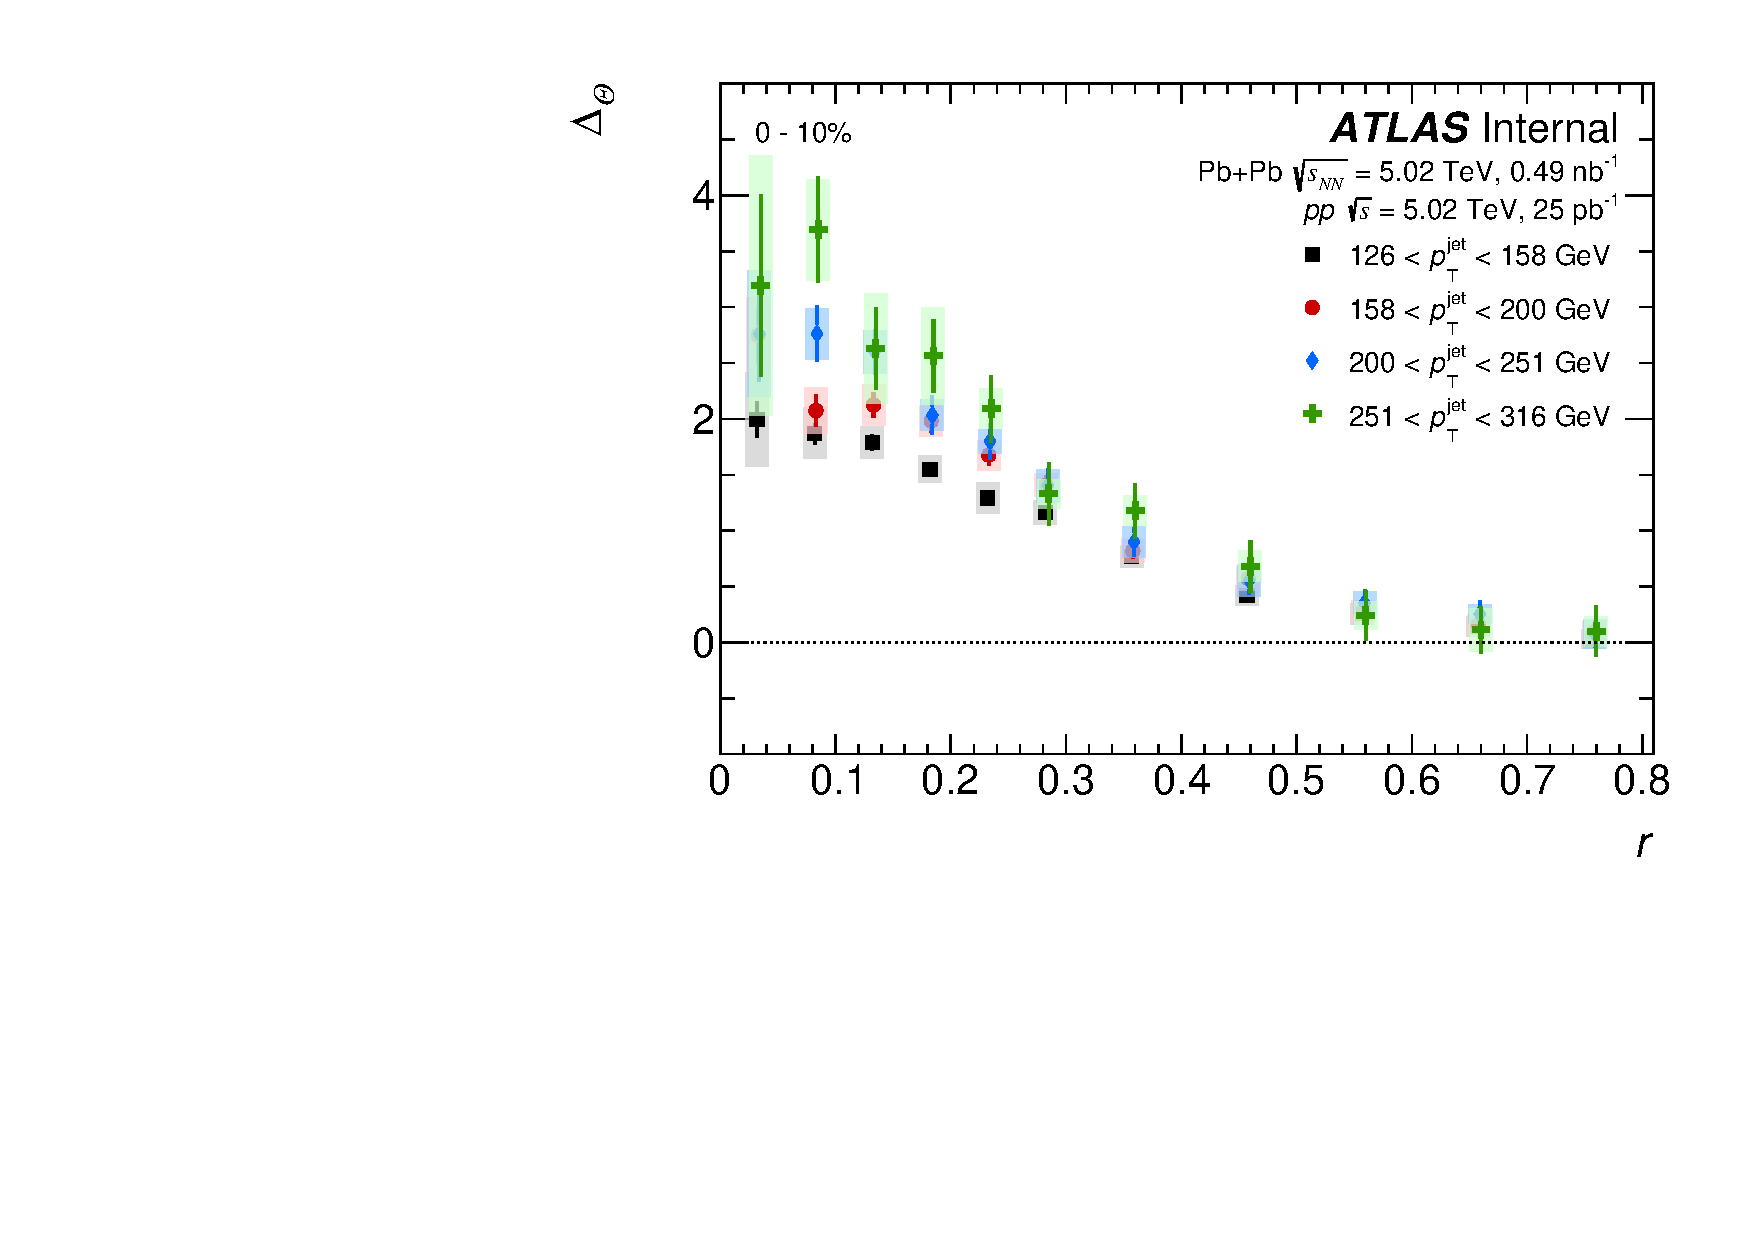
\includegraphics[width=0.5\textwidth]{results/DeltaDpT_lowpt_integ_cent0.pdf} &
	 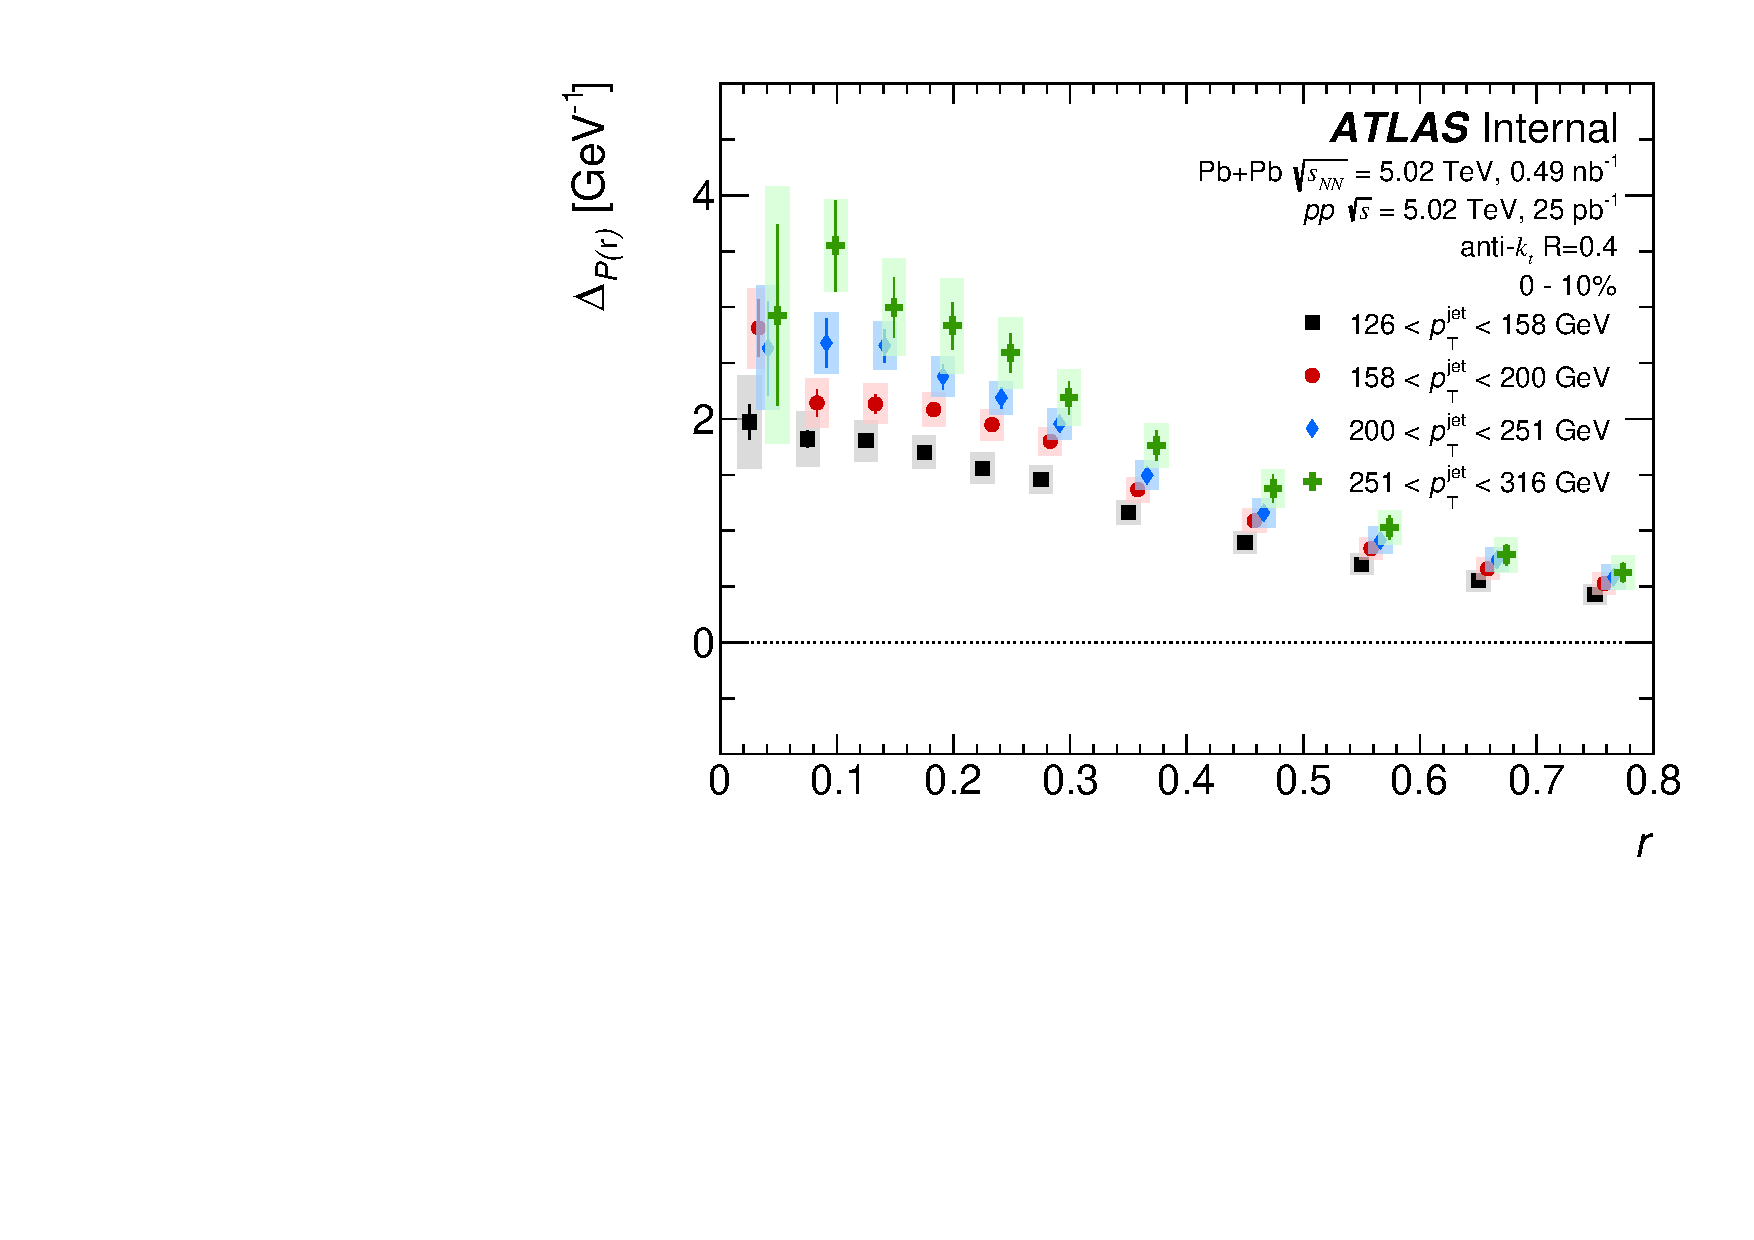
\includegraphics[width=0.5\textwidth]{results/DeltaDpT_jetshape_cent0.pdf} \\
	 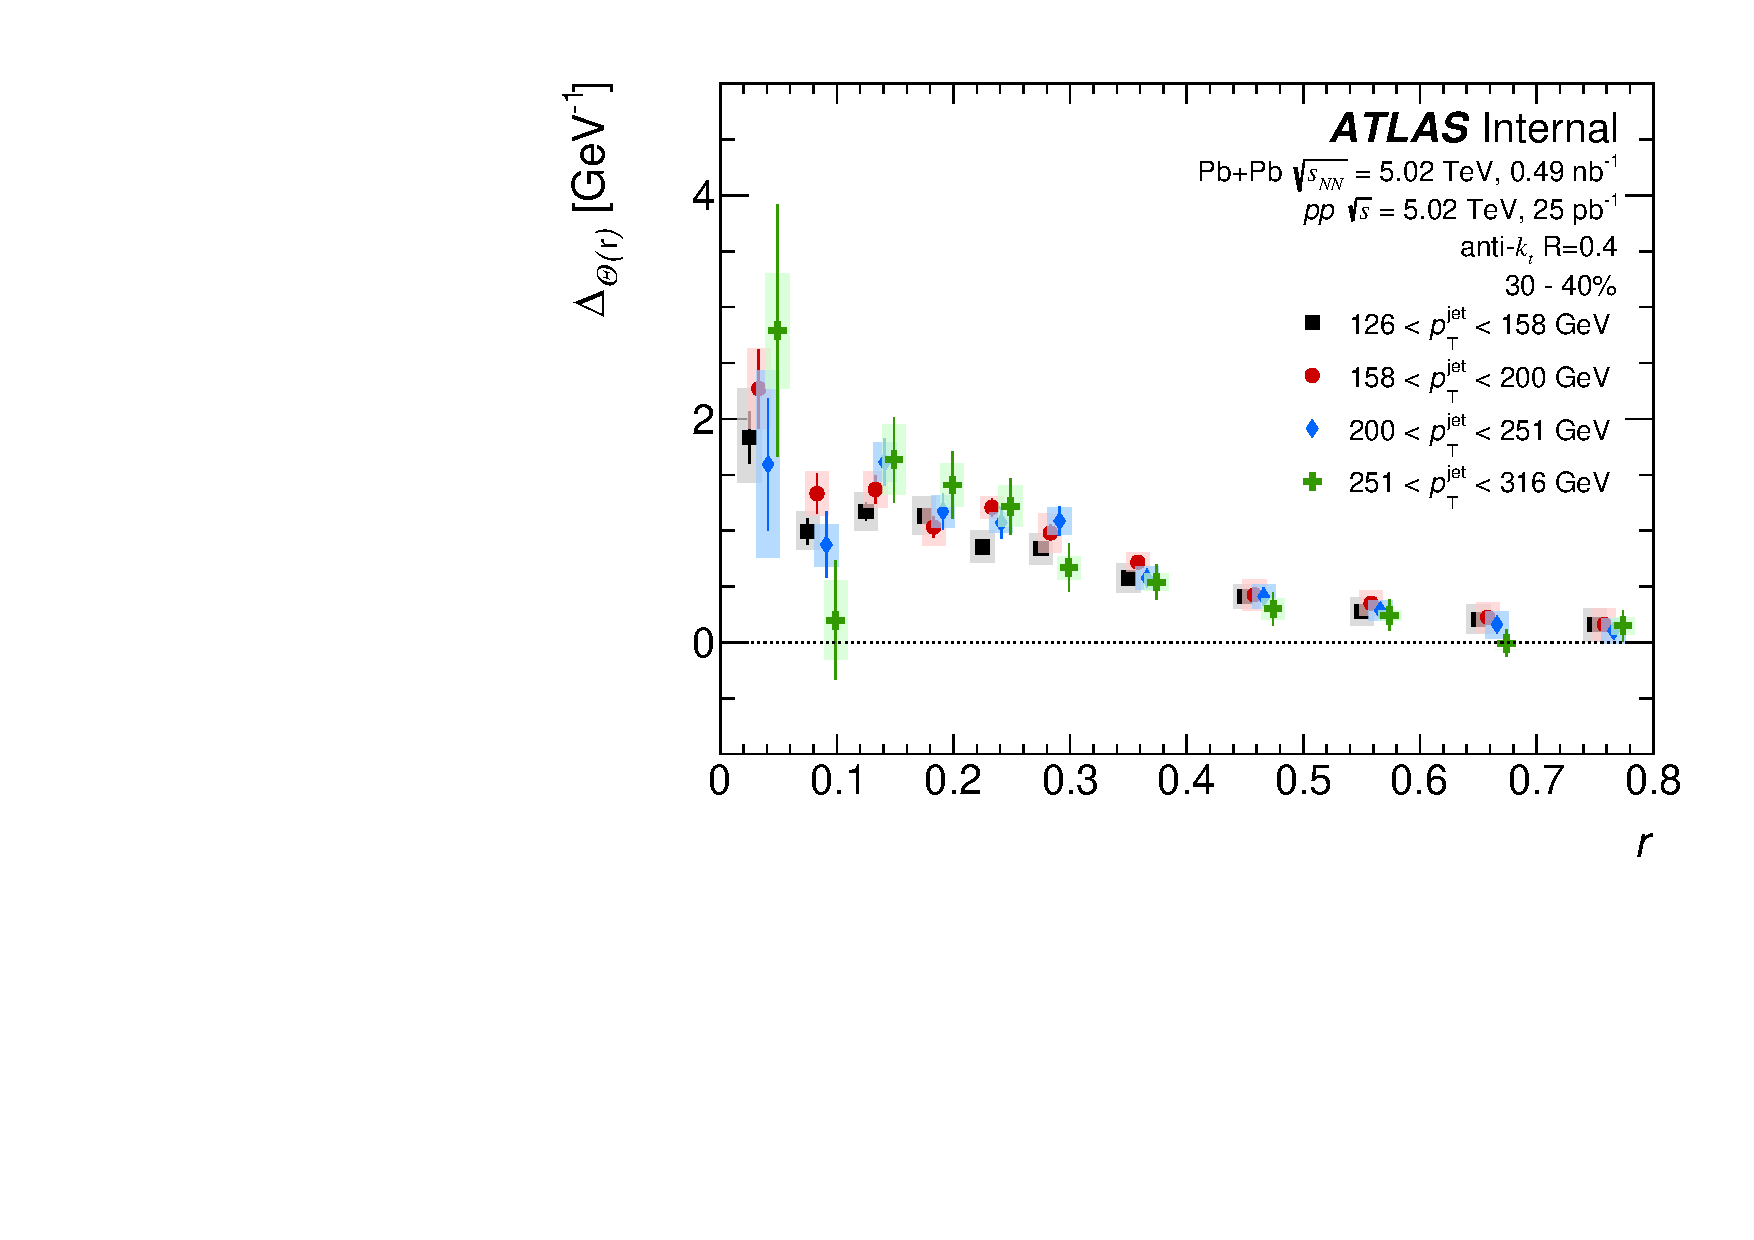
\includegraphics[width=0.5\textwidth]{results/DeltaDpT_lowpt_integ_cent3.pdf} &
	 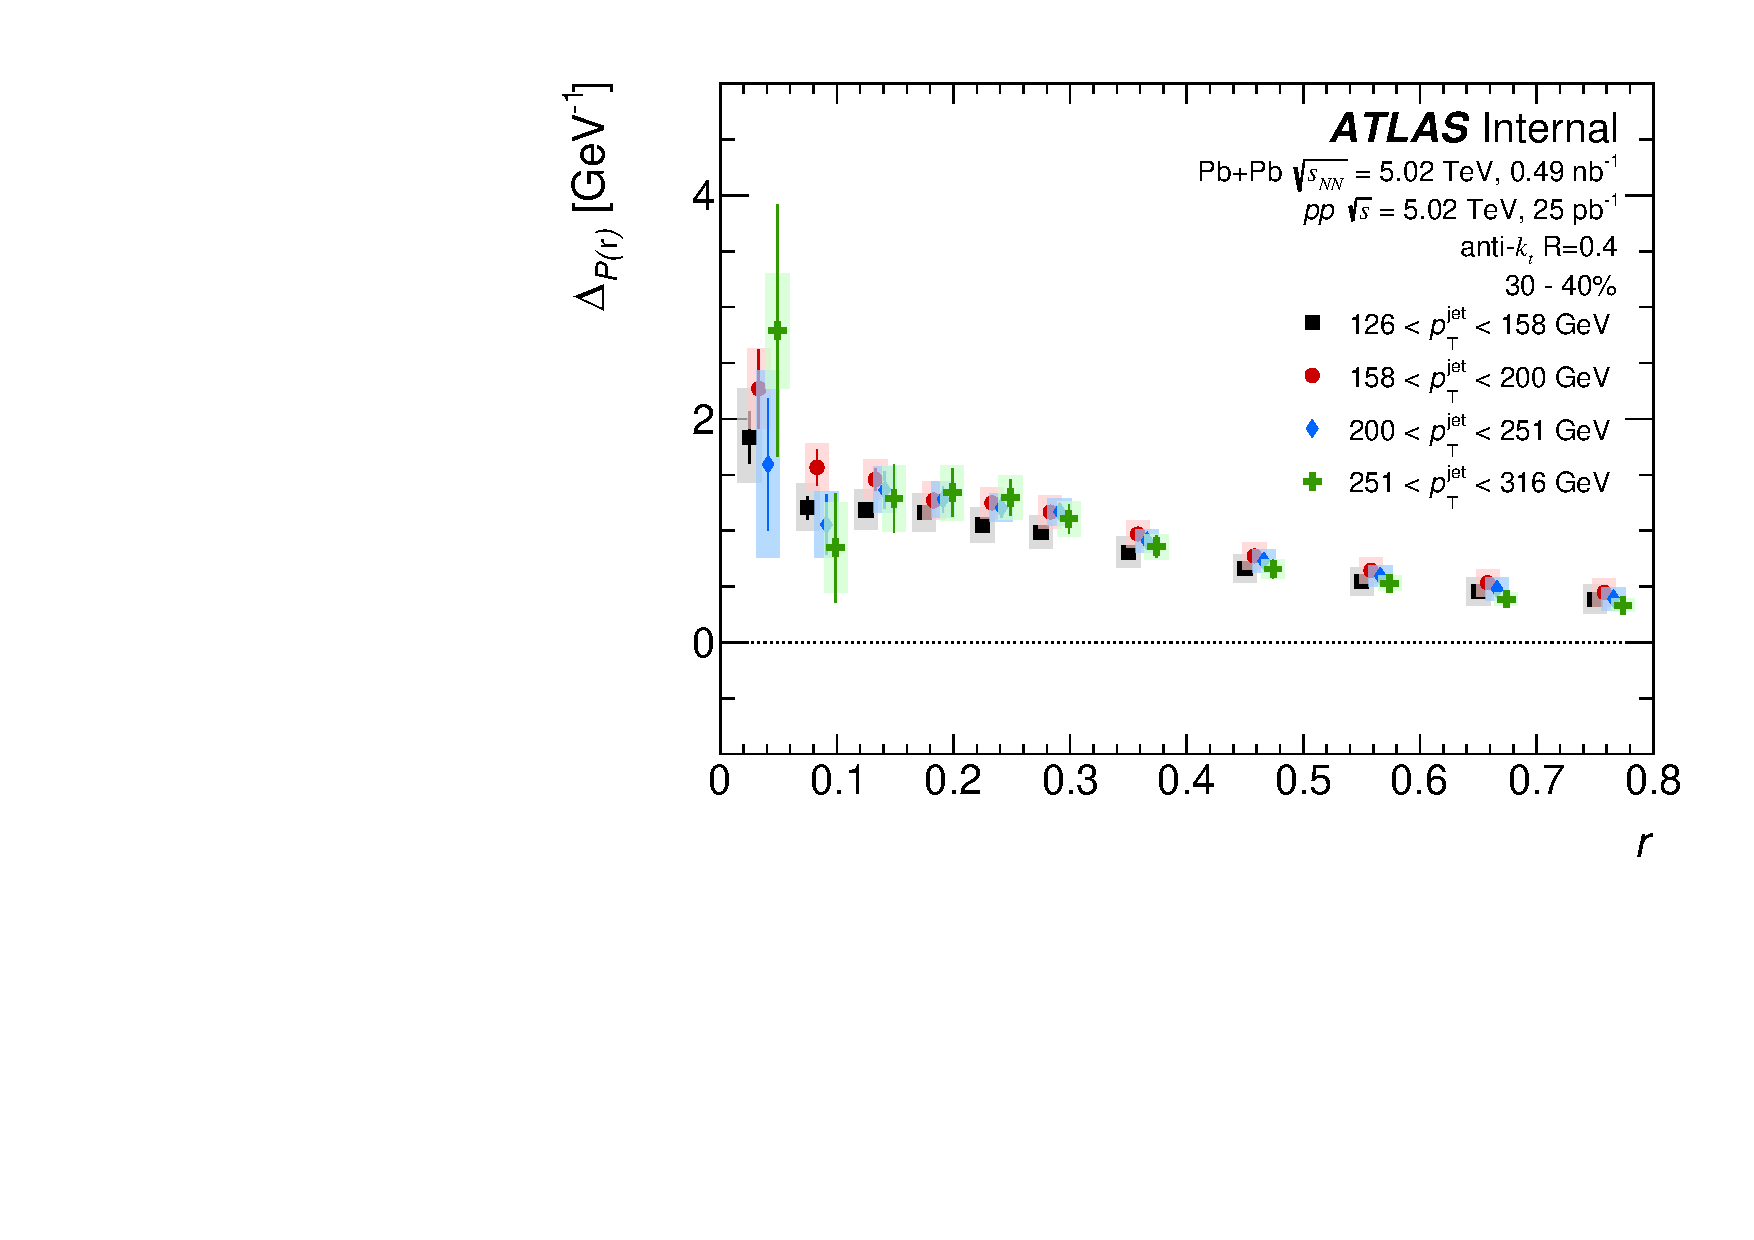
\includegraphics[width=0.5\textwidth]{results/DeltaDpT_jetshape_cent3.pdf} \\
	 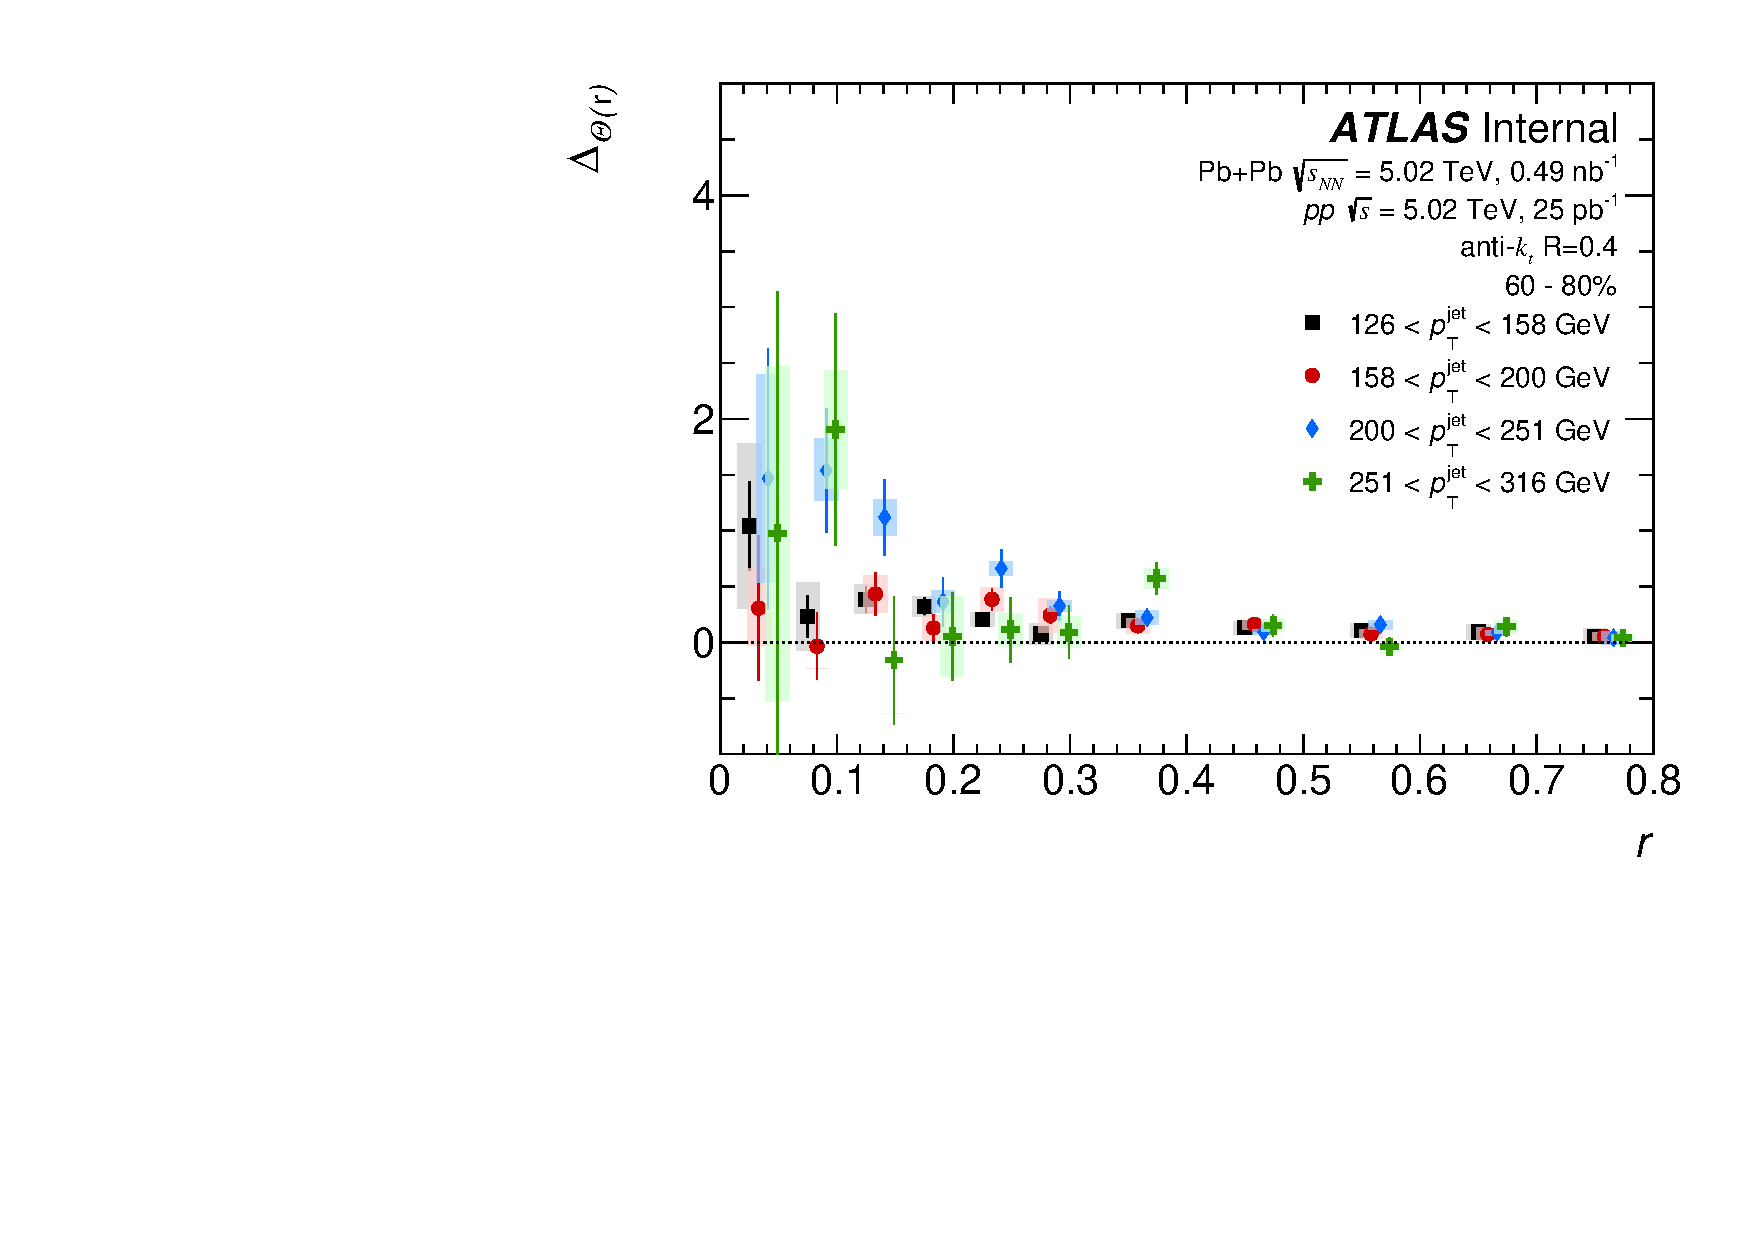
\includegraphics[width=0.5\textwidth]{results/DeltaDpT_lowpt_integ_cent5.pdf} &
	 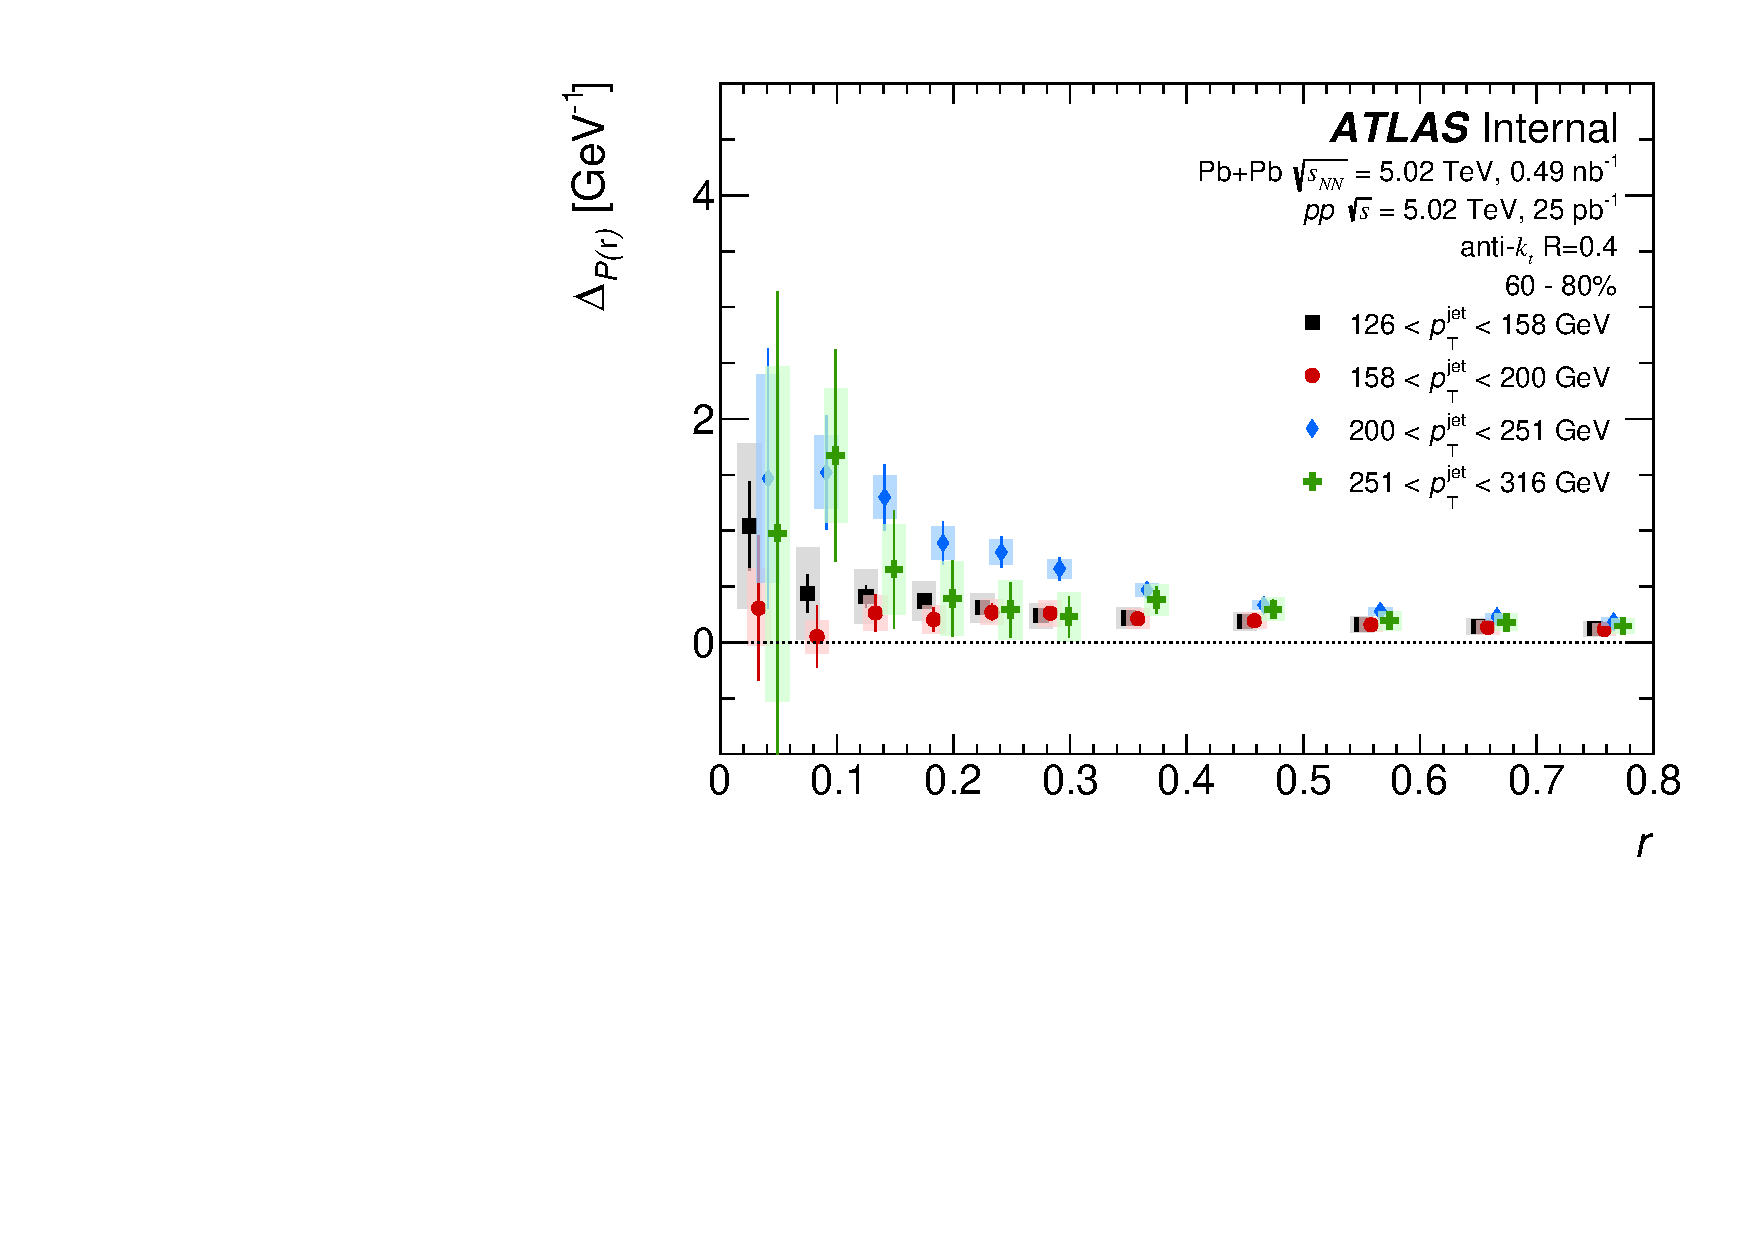
\includegraphics[width=0.5\textwidth]{results/DeltaDpT_jetshape_cent5.pdf} \\
\end{tabular} }
   \caption{\DeltaTheta\ (left) and \DeltaP\ (right) as a function of \rvar\ in central collisions for charged-particles with \pt\ < 4 GeV ranges in four \ptjet\ selections: 126--158~\GeV, 158--200~\GeV, 200--251~\GeV, and 251--316~\GeV and three centrality selections: 0--10\% (top), 30--40\% (middle) and 60--80\% (bottom). The vertical bars on the data points indicate statistical uncertainties while the shaded boxes indicate systematic uncertainties. The widths of the boxes are not indicative of the bin size and the points are shifted horizontally for better visibility. }
      \label{fig:deltaPdeltaT}
\end{figure}


\begin{figure}
\centering{
\begin{tabular}{cc}
	 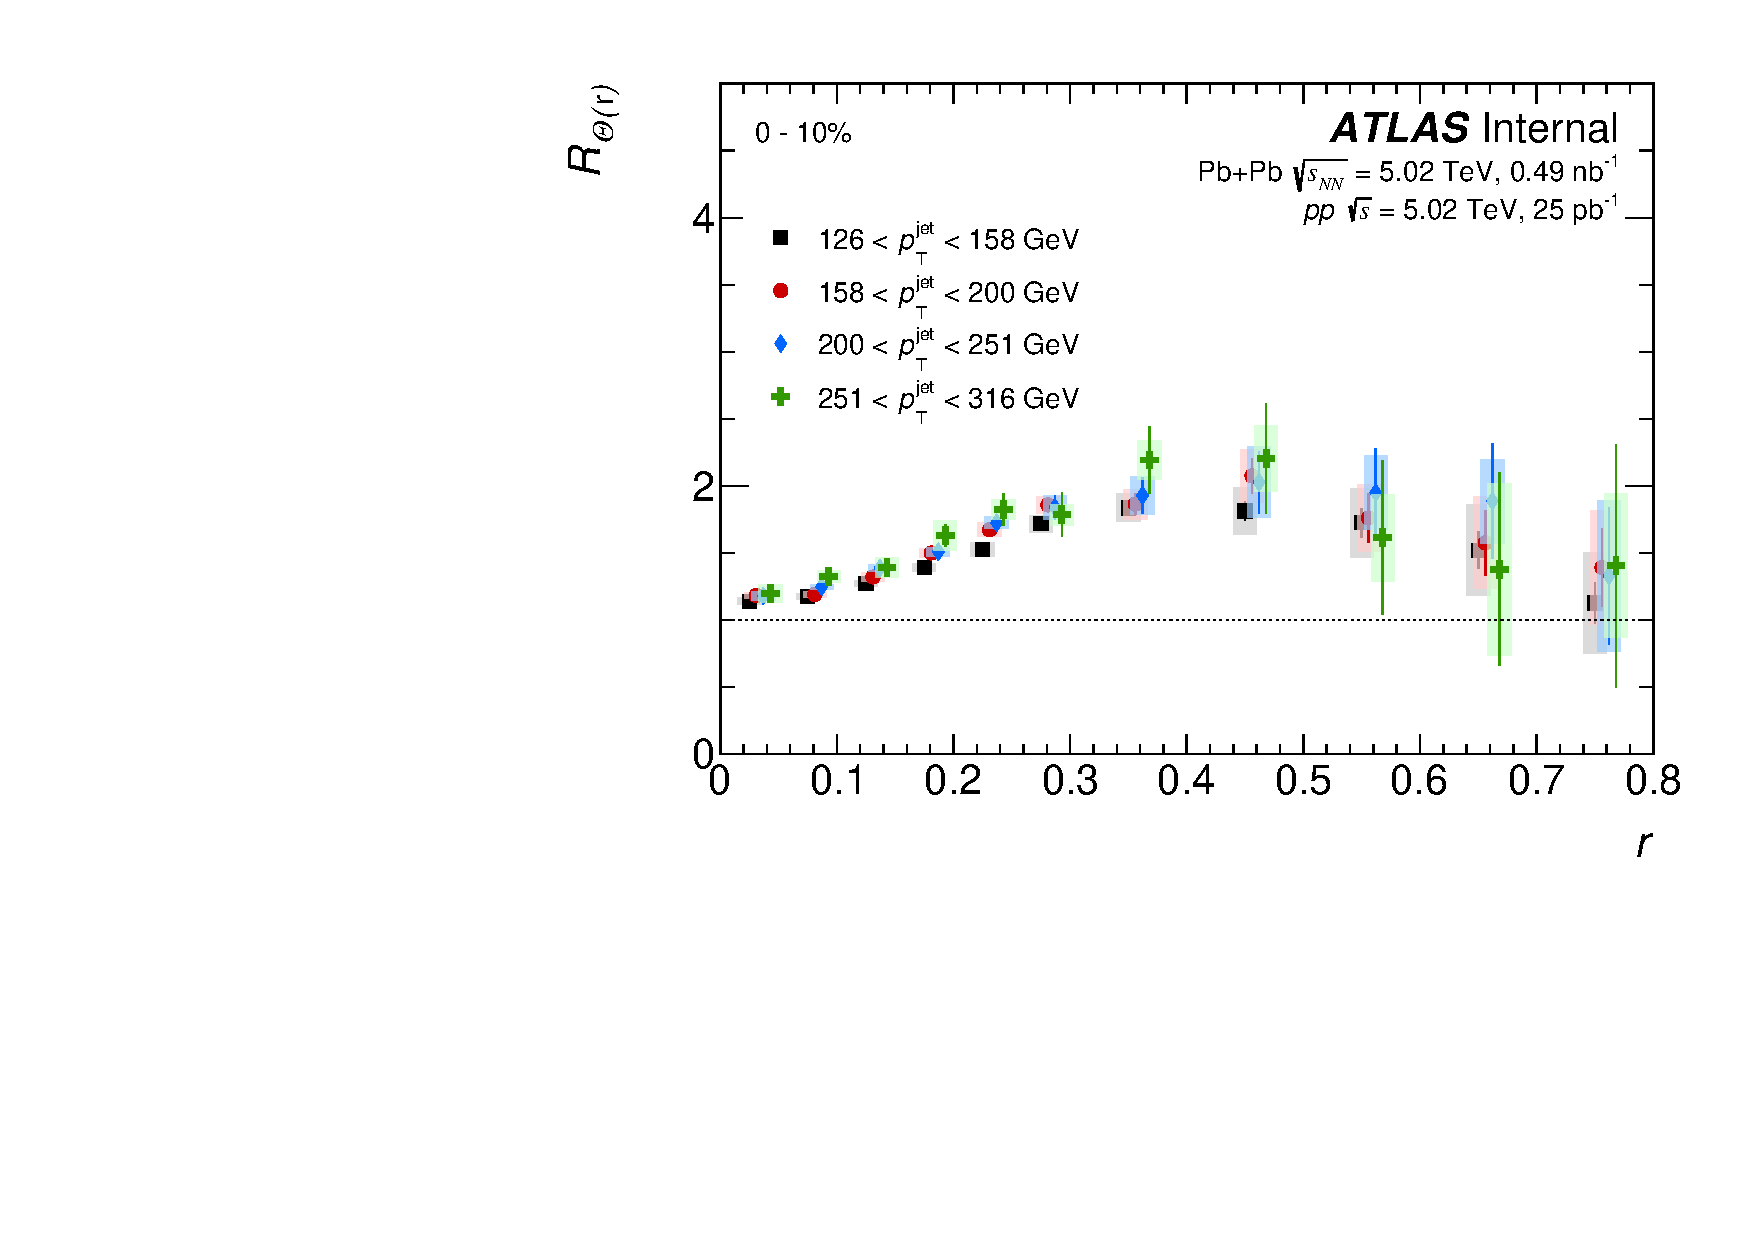
\includegraphics[width=0.5\textwidth]{results/RDpT_lowpt_integ_cent0.pdf} &
	 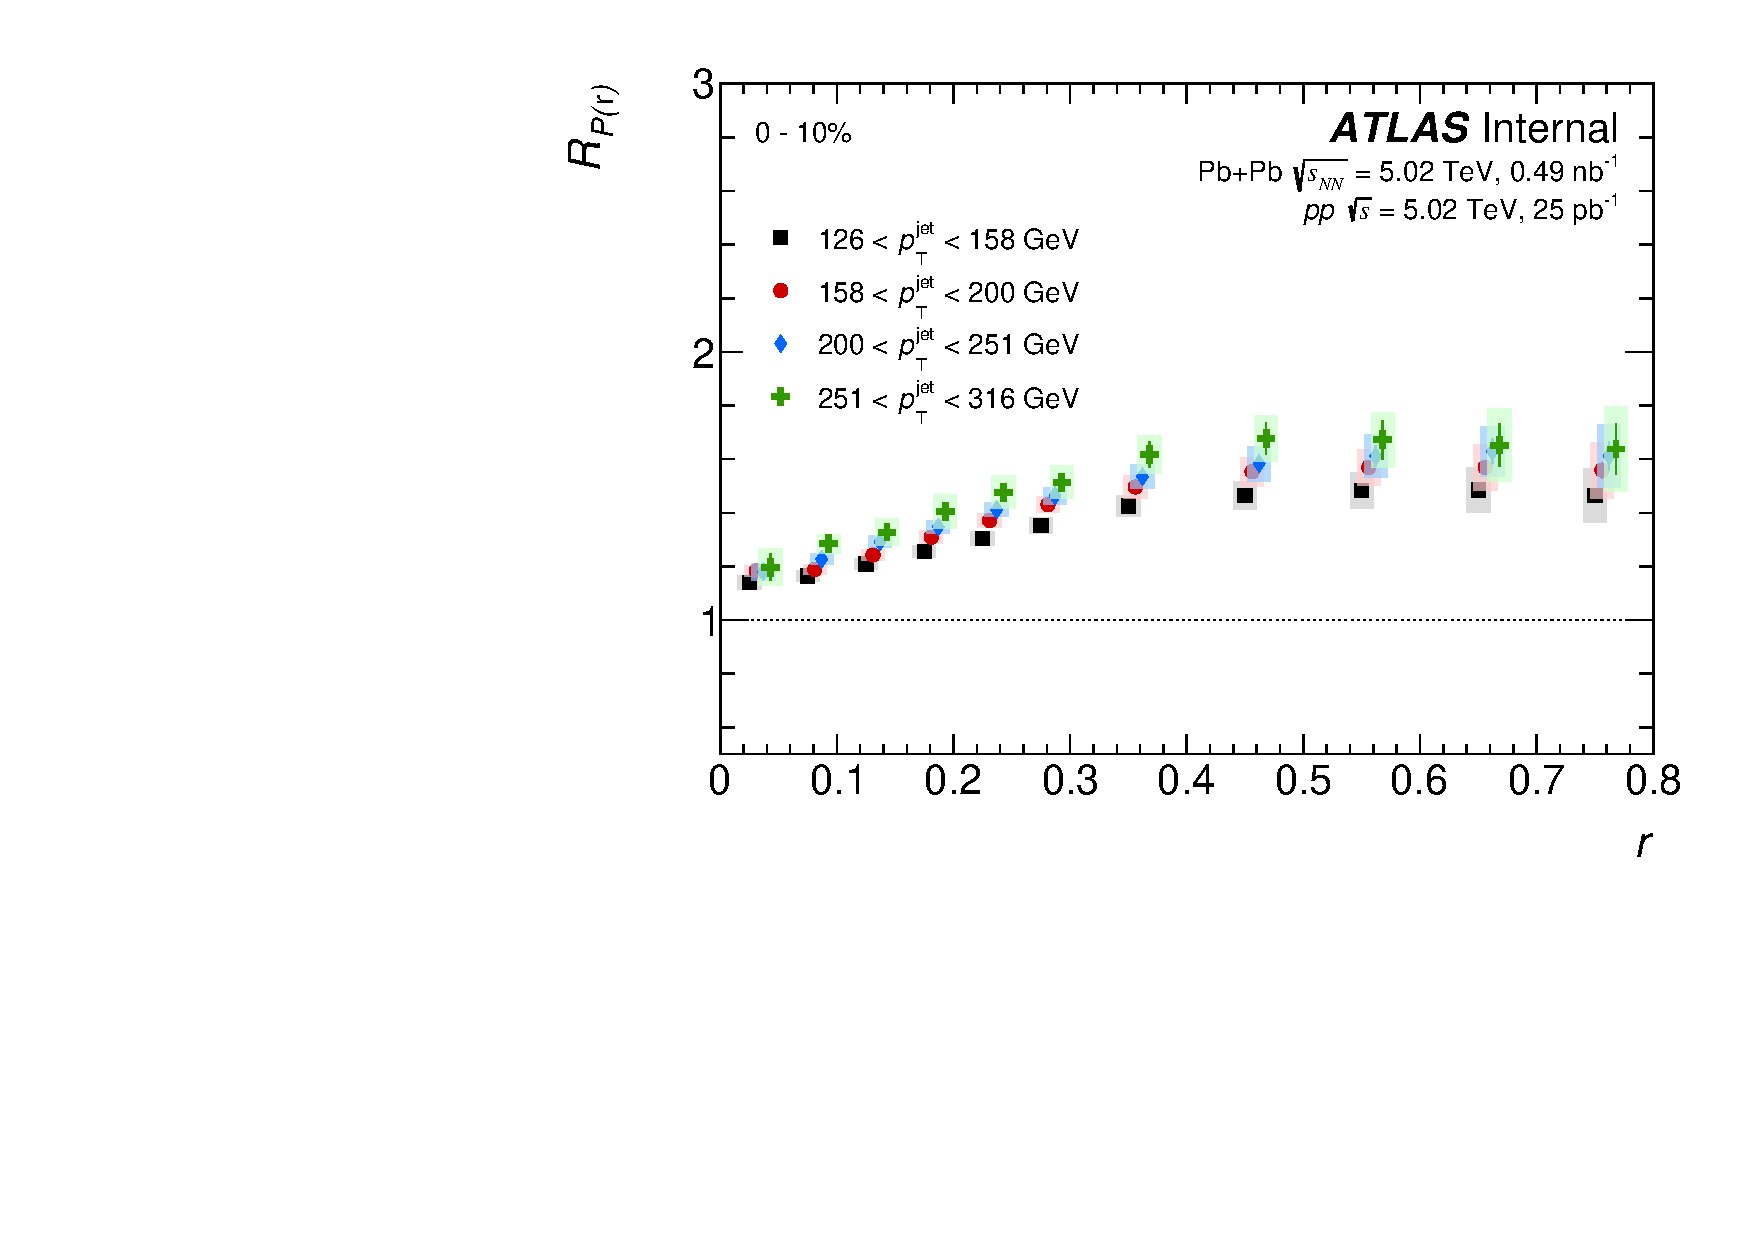
\includegraphics[width=0.5\textwidth]{results/RDpT_jetshape_cent0.pdf} \\
	 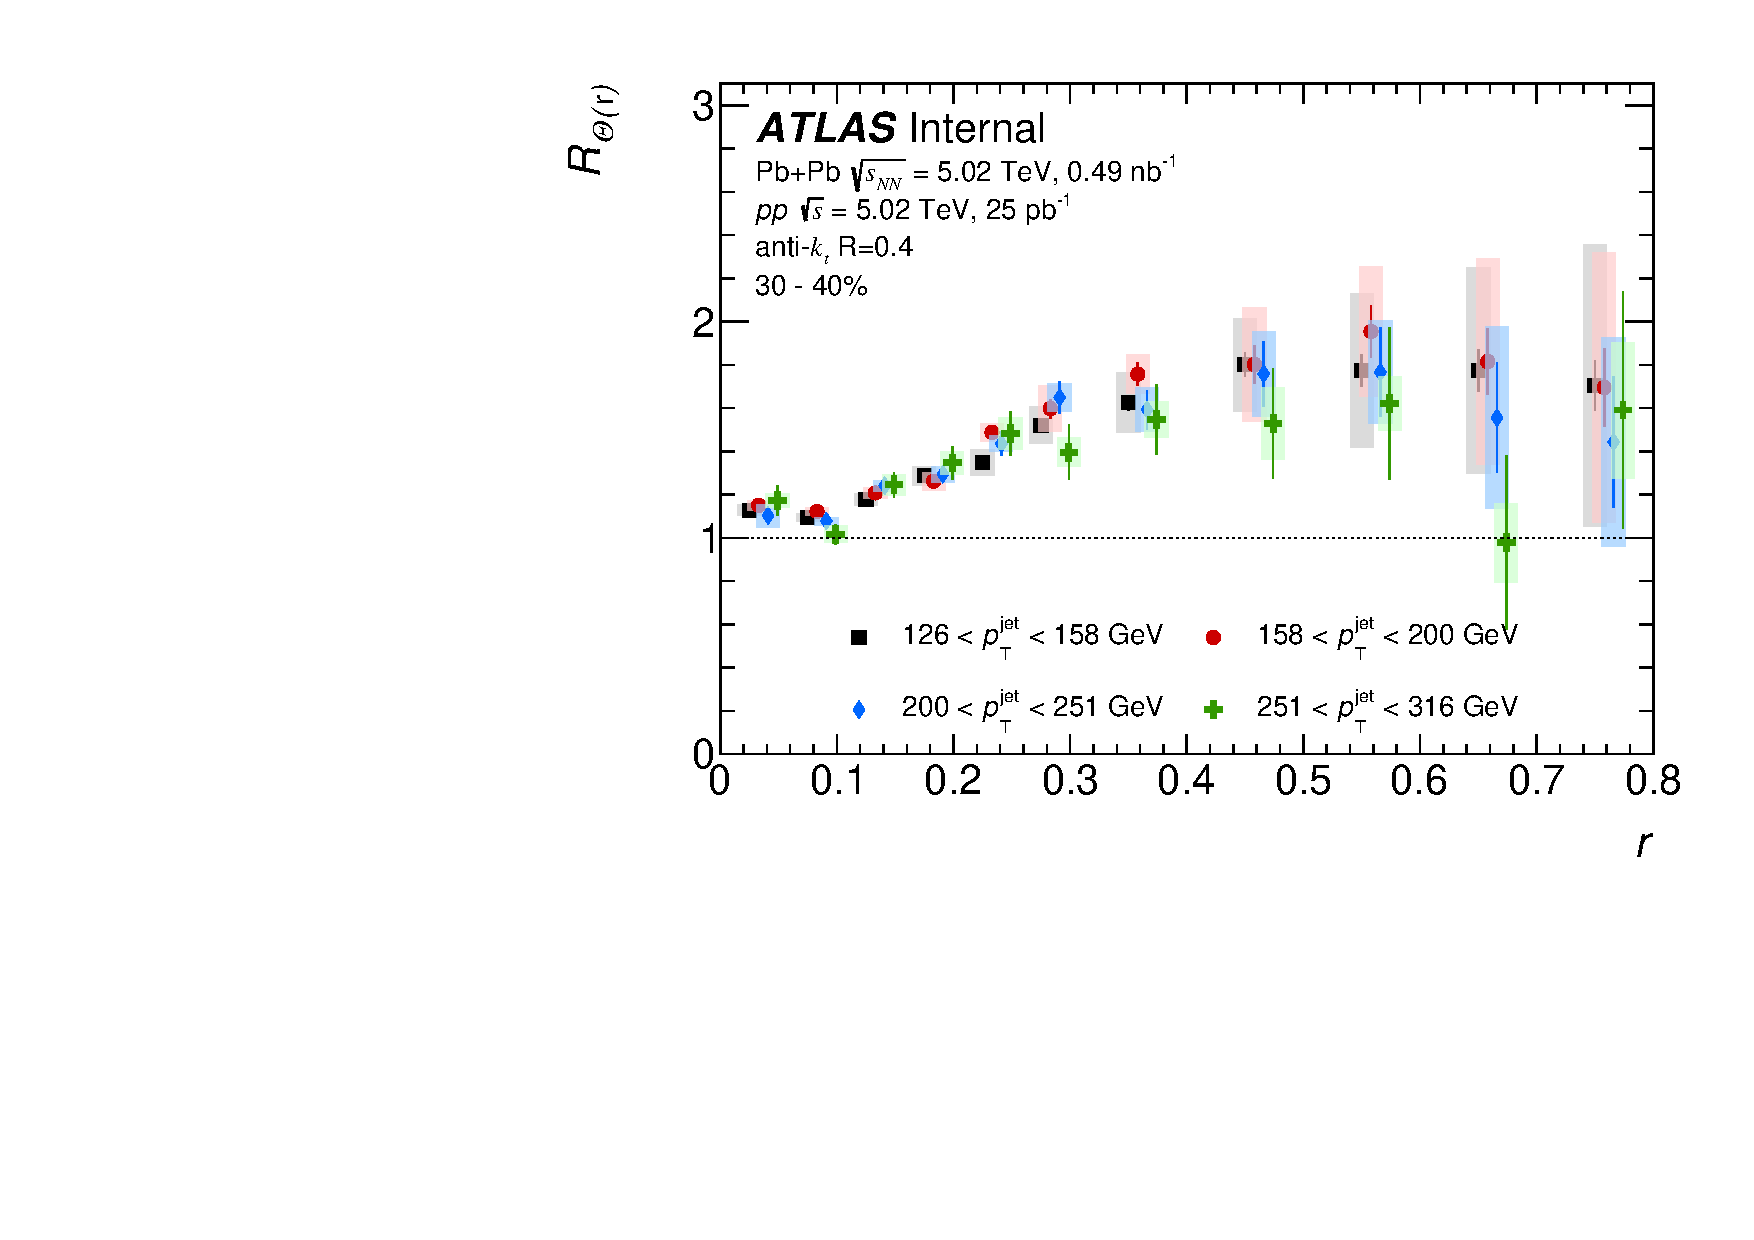
\includegraphics[width=0.5\textwidth]{results/RDpT_lowpt_integ_cent3.pdf} &
	 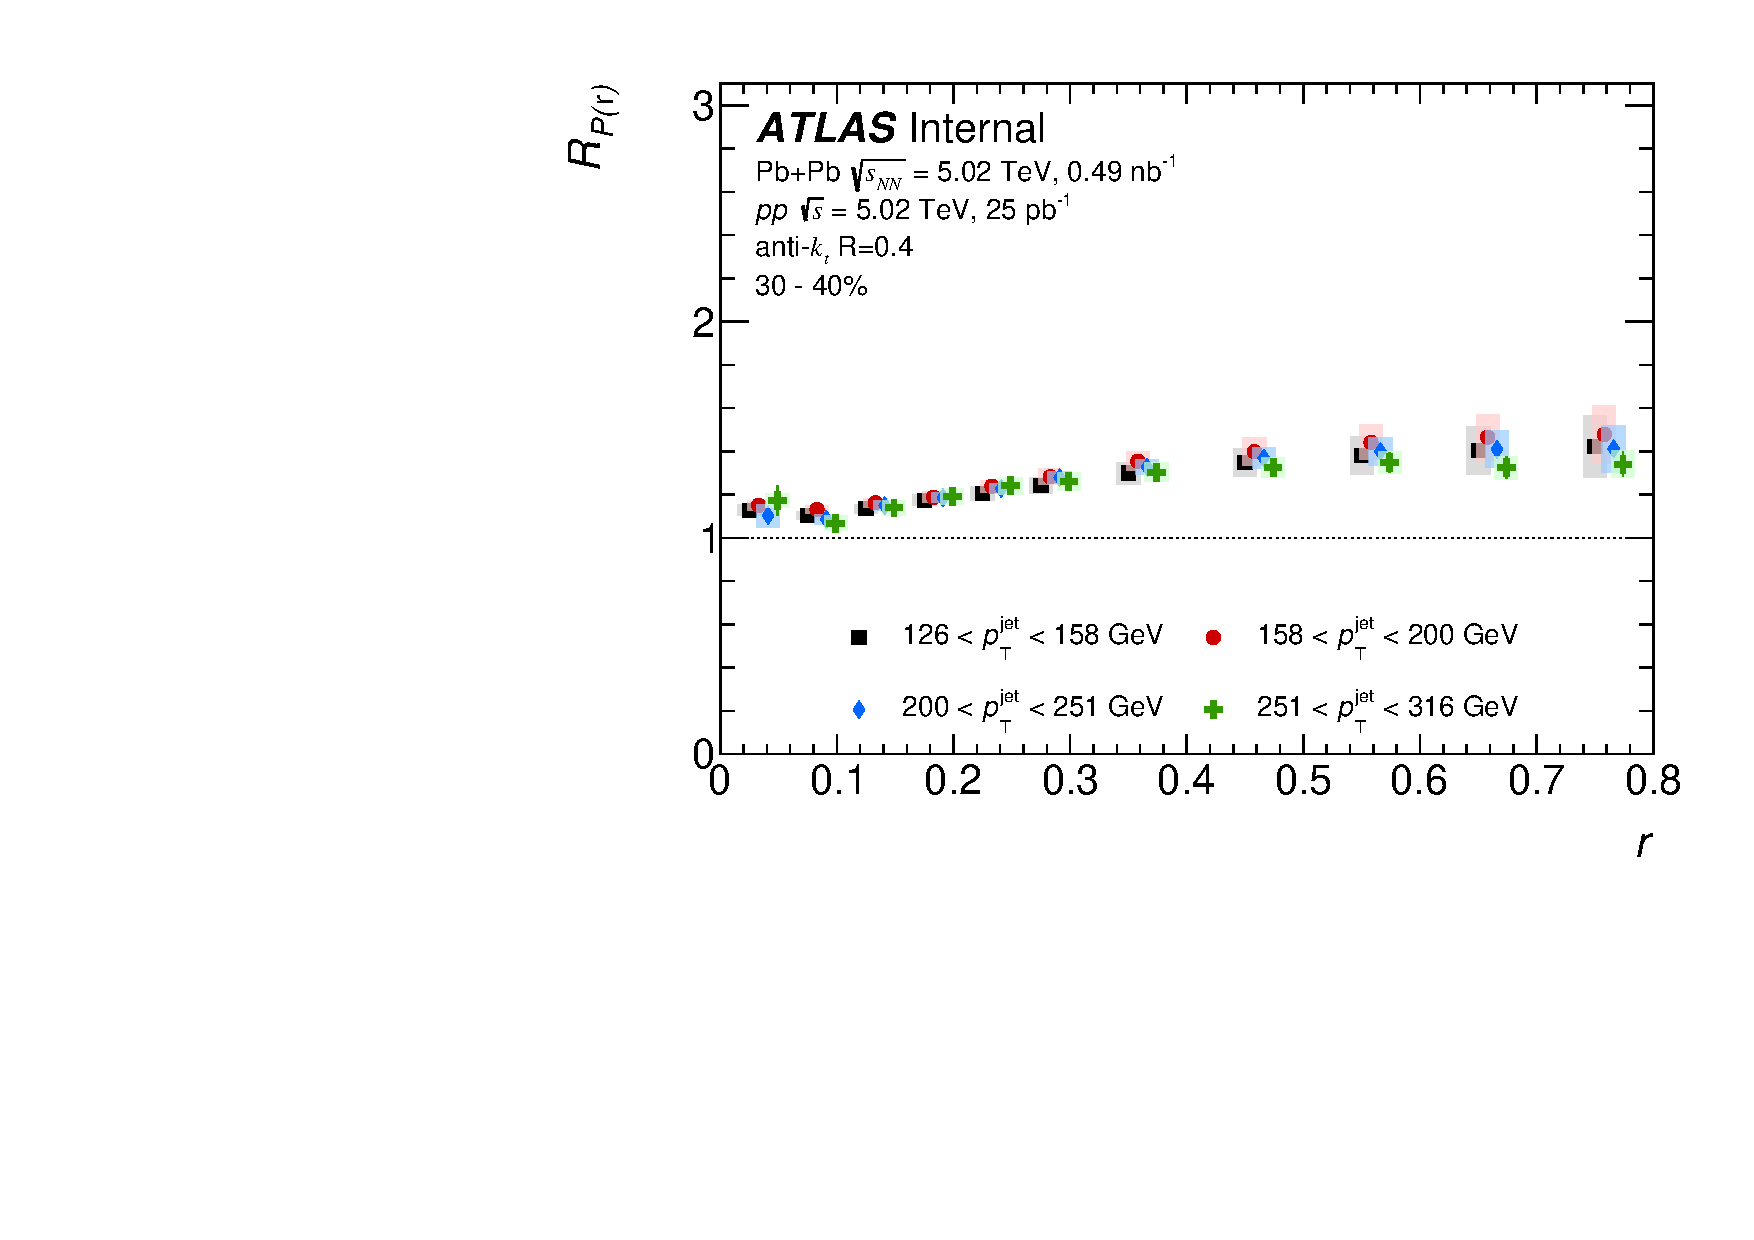
\includegraphics[width=0.5\textwidth]{results/RDpT_jetshape_cent3.pdf} \\
	 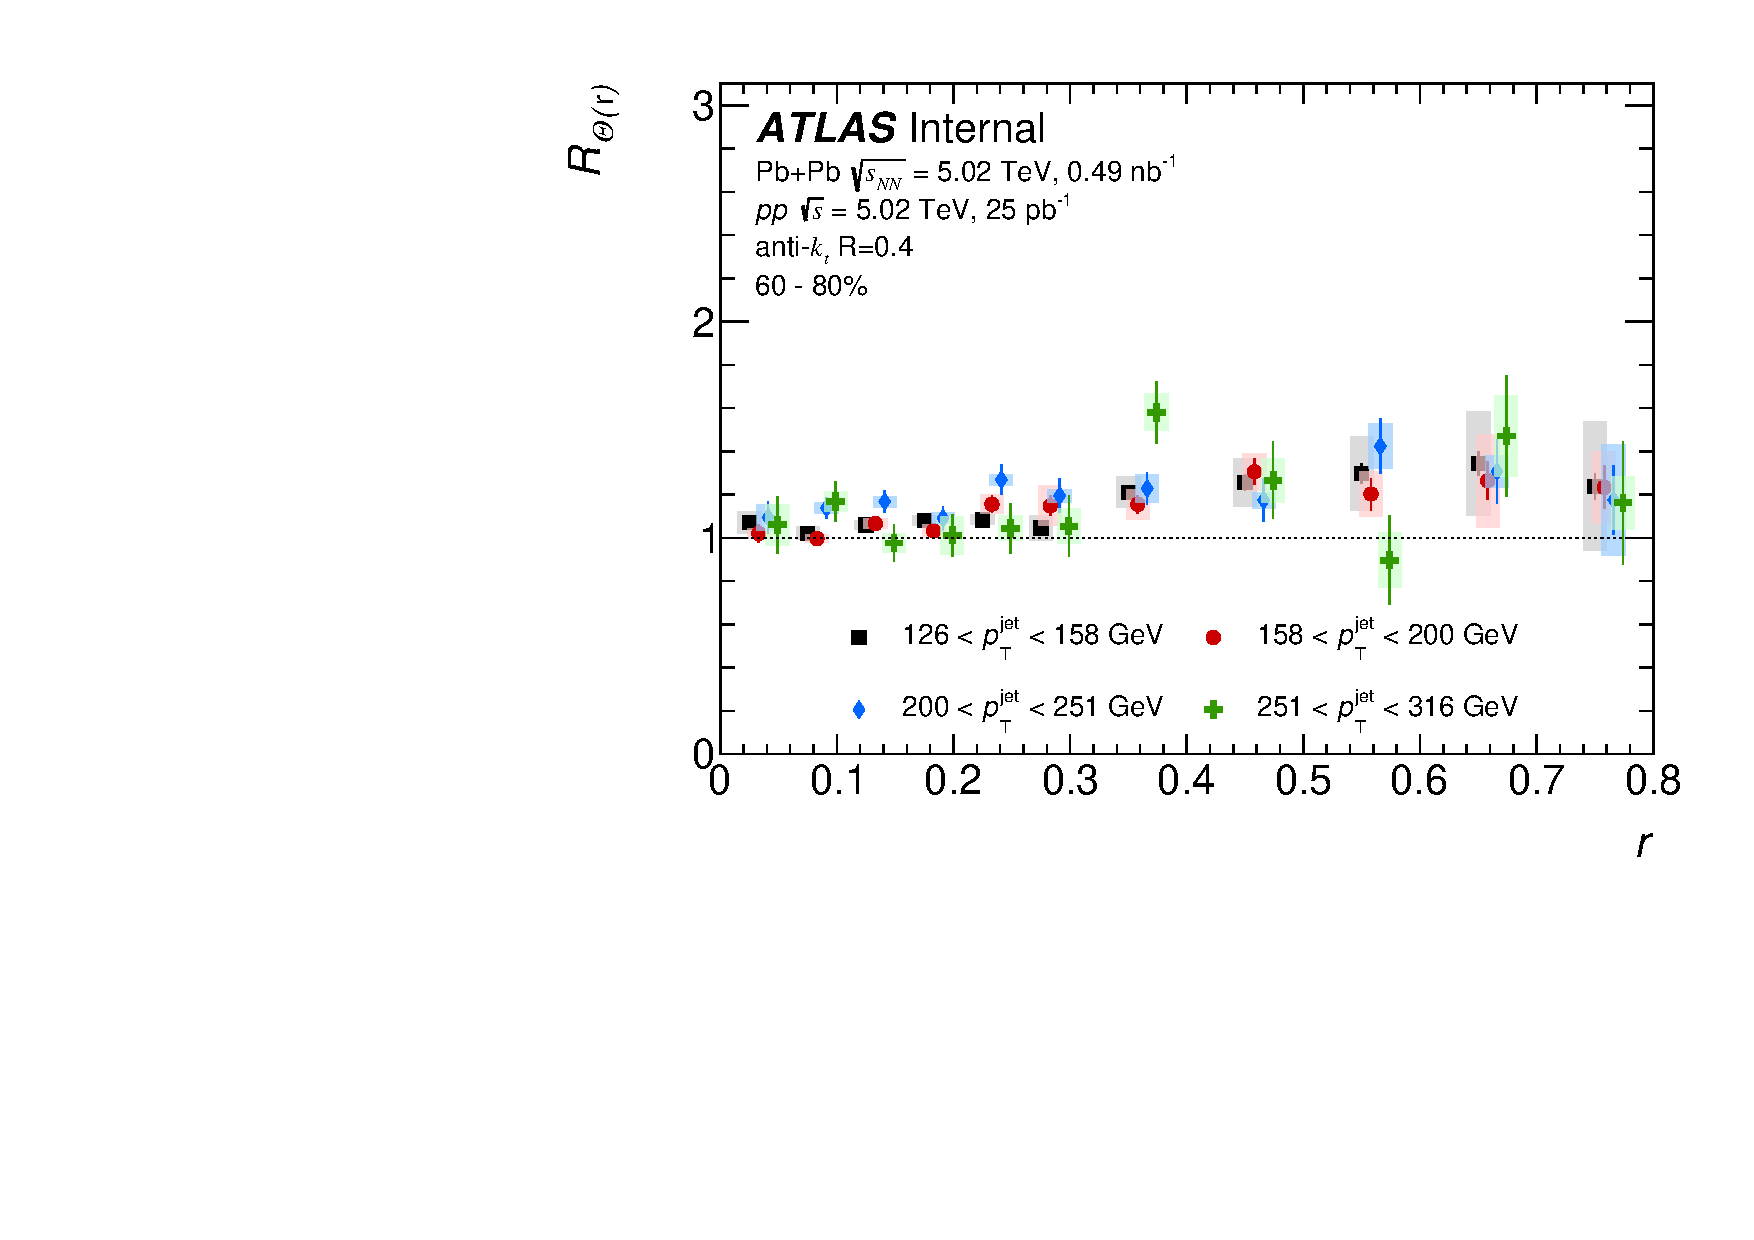
\includegraphics[width=0.5\textwidth]{results/RDpT_lowpt_integ_cent5.pdf} &
	 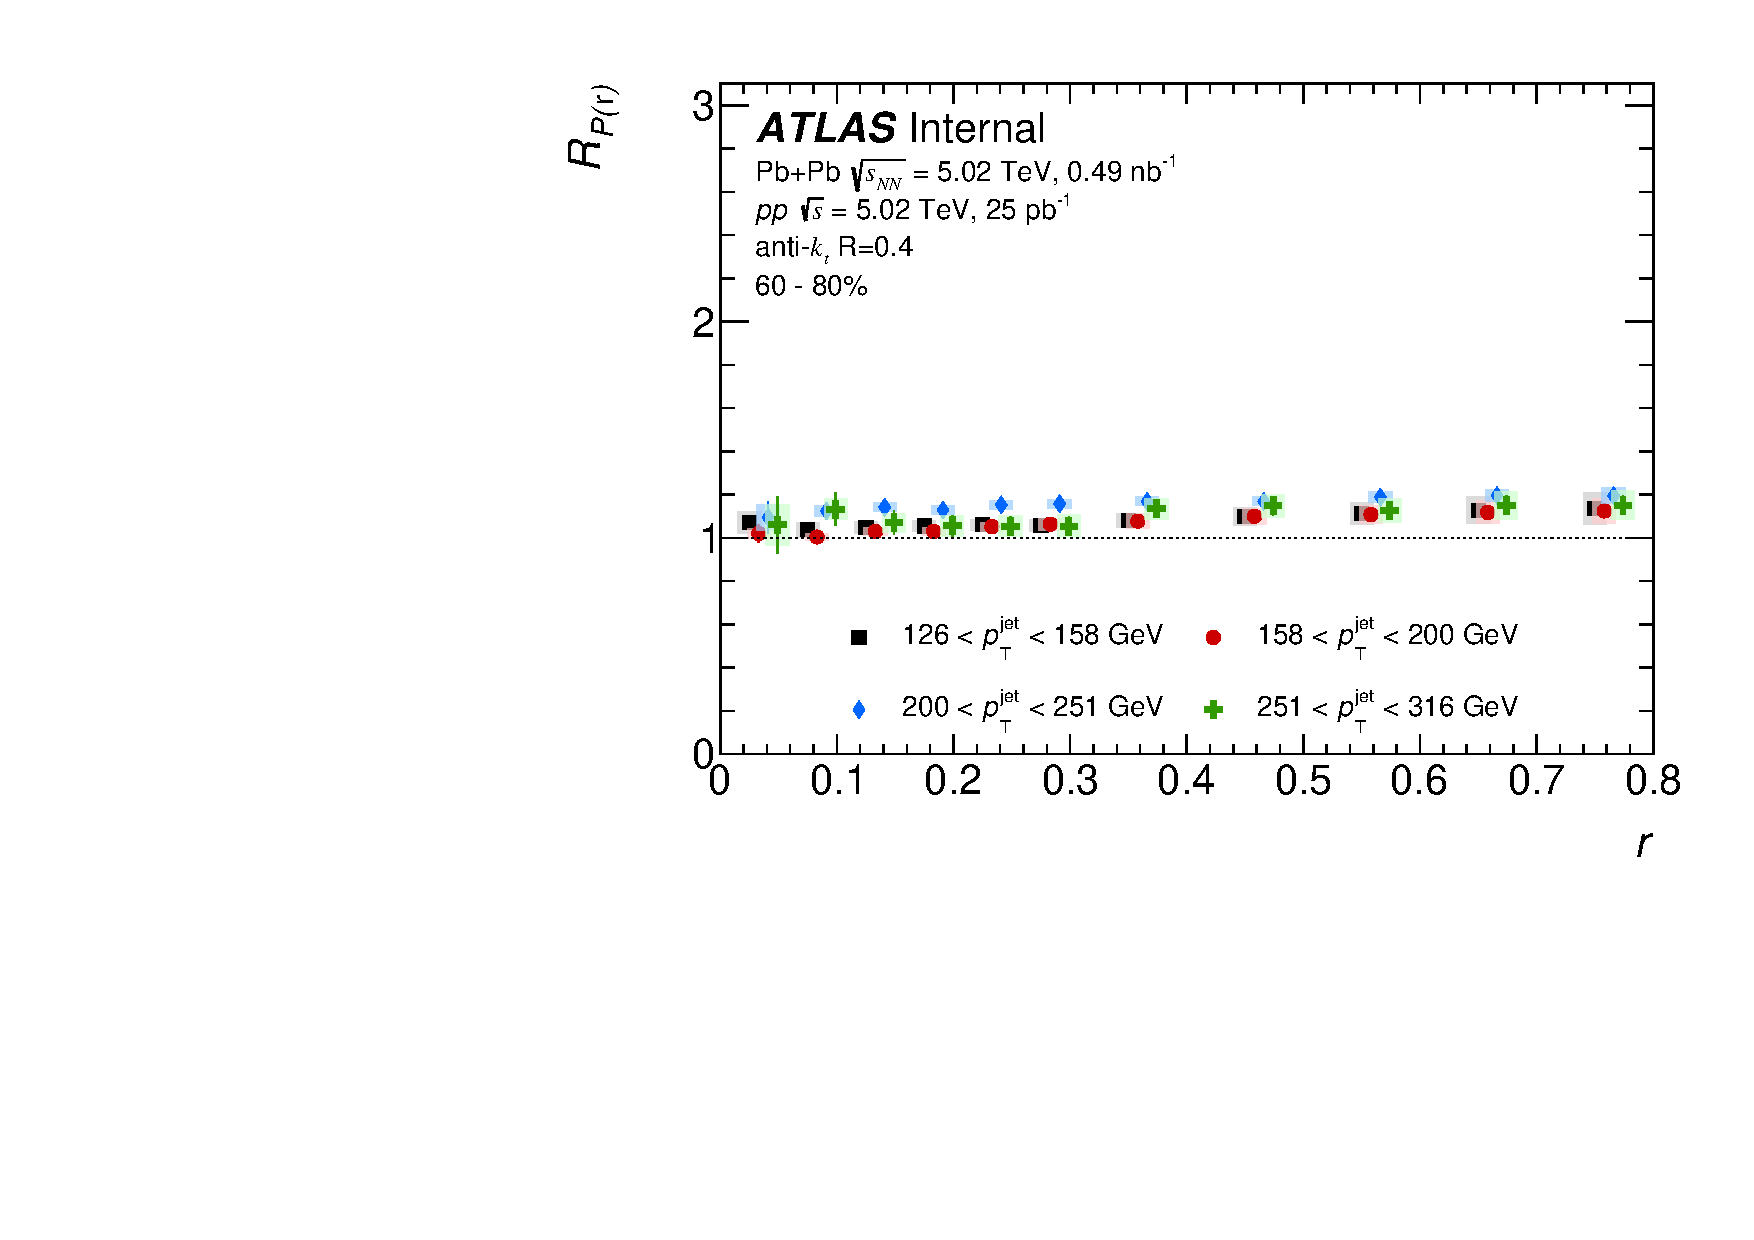
\includegraphics[width=0.5\textwidth]{results/RDpT_jetshape_cent5.pdf} \\
\end{tabular} }
   \caption{\RTheta\ (left) and \RP\ (right) as a function of \rvar\ in central collisions for charged-particles with \pt\ < 4 GeV ranges in four \ptjet\ selections: 126--158~\GeV, 158--200~\GeV, 200--251~\GeV, and 251--316~\GeV and three centrality selections: 0--10\% (top), 30--40\% (middle) and 60--80\% (bottom). The vertical bars on the data points indicate statistical uncertainties while the shaded boxes indicate systematic uncertainties. The widths of the boxes are not indicative of the bin size and the points are shifted horizontally for better visibility. }
      \label{fig:RPRT}
\end{figure}



%
%%% RDpT as function of jet pT
%\begin{figure}
%\centering{
%\begin{tabular}{cc}
%	 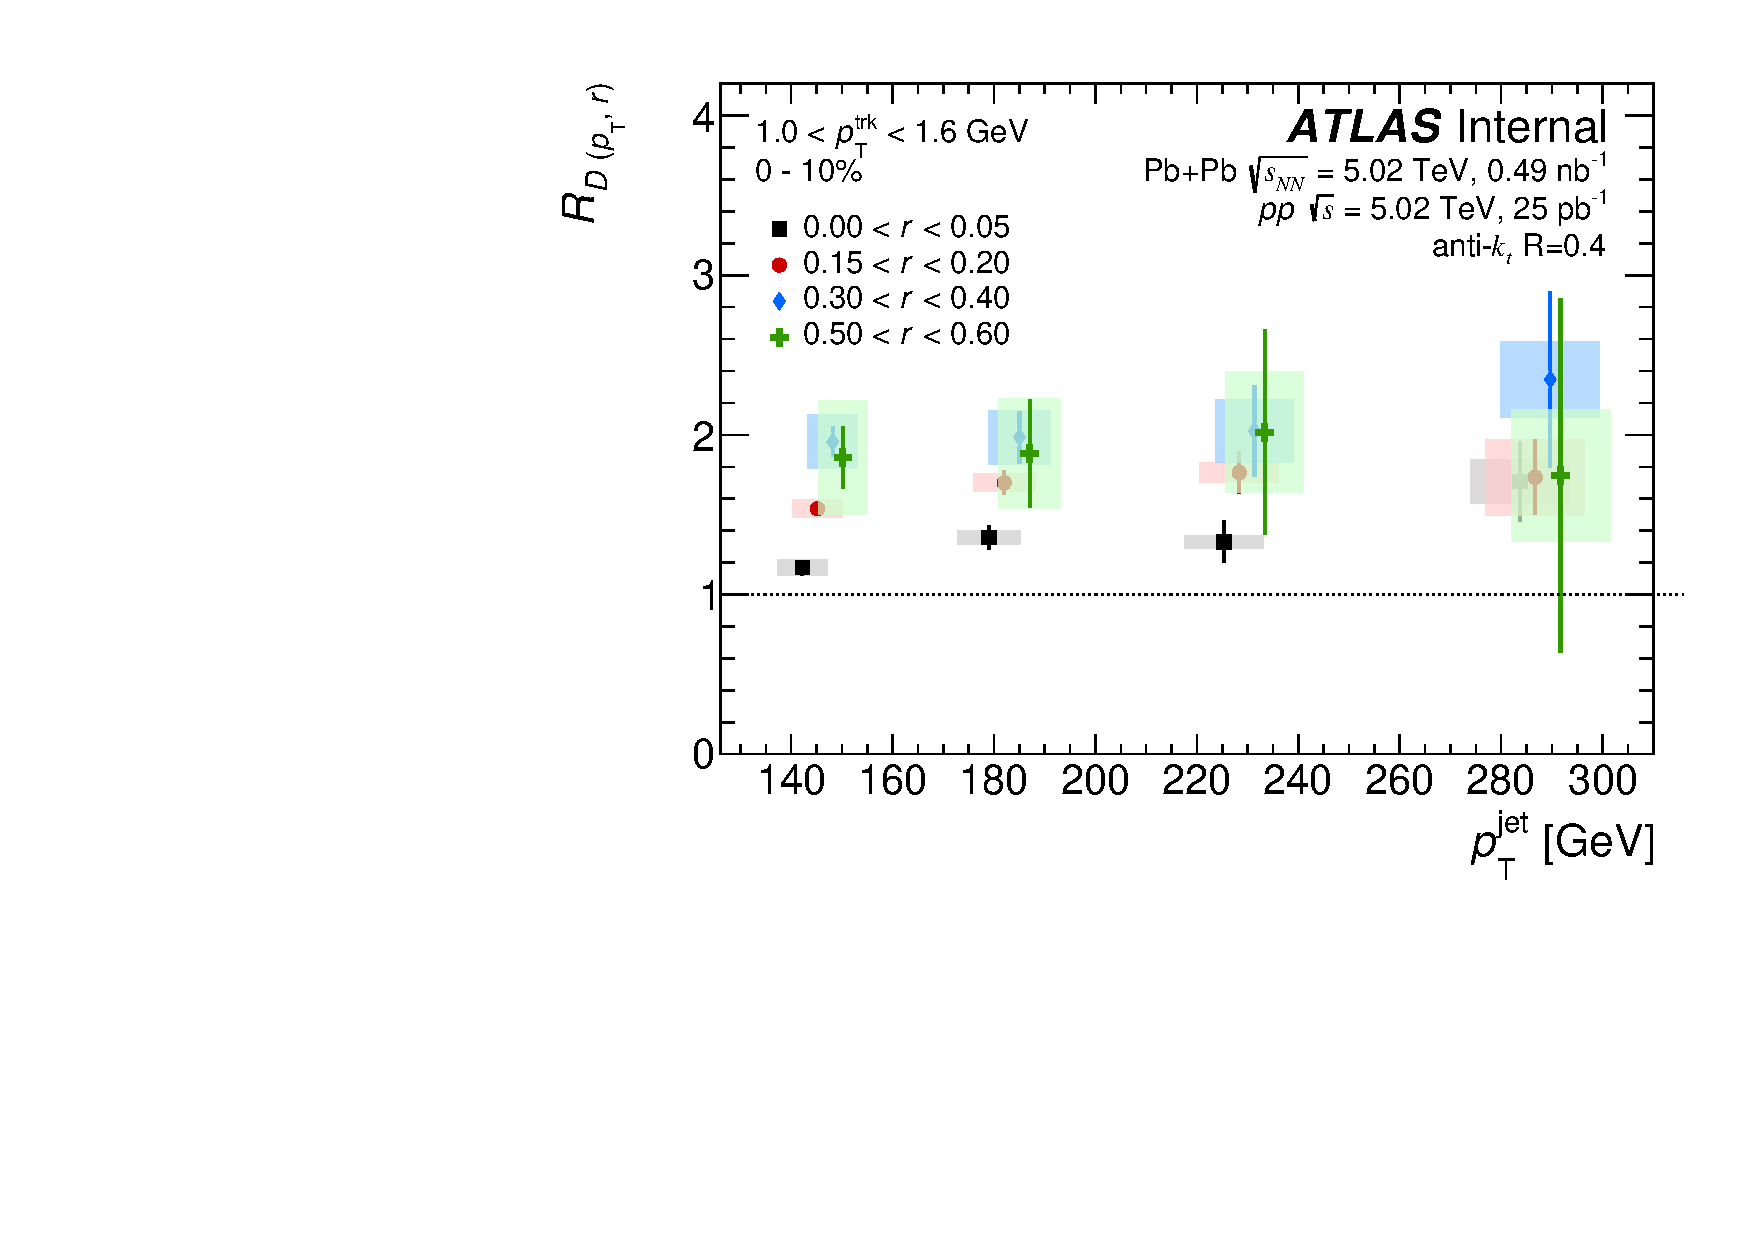
\includegraphics[width=0.45\textwidth]{results/RDpT_jetpt_trk2_cent0} &
%	 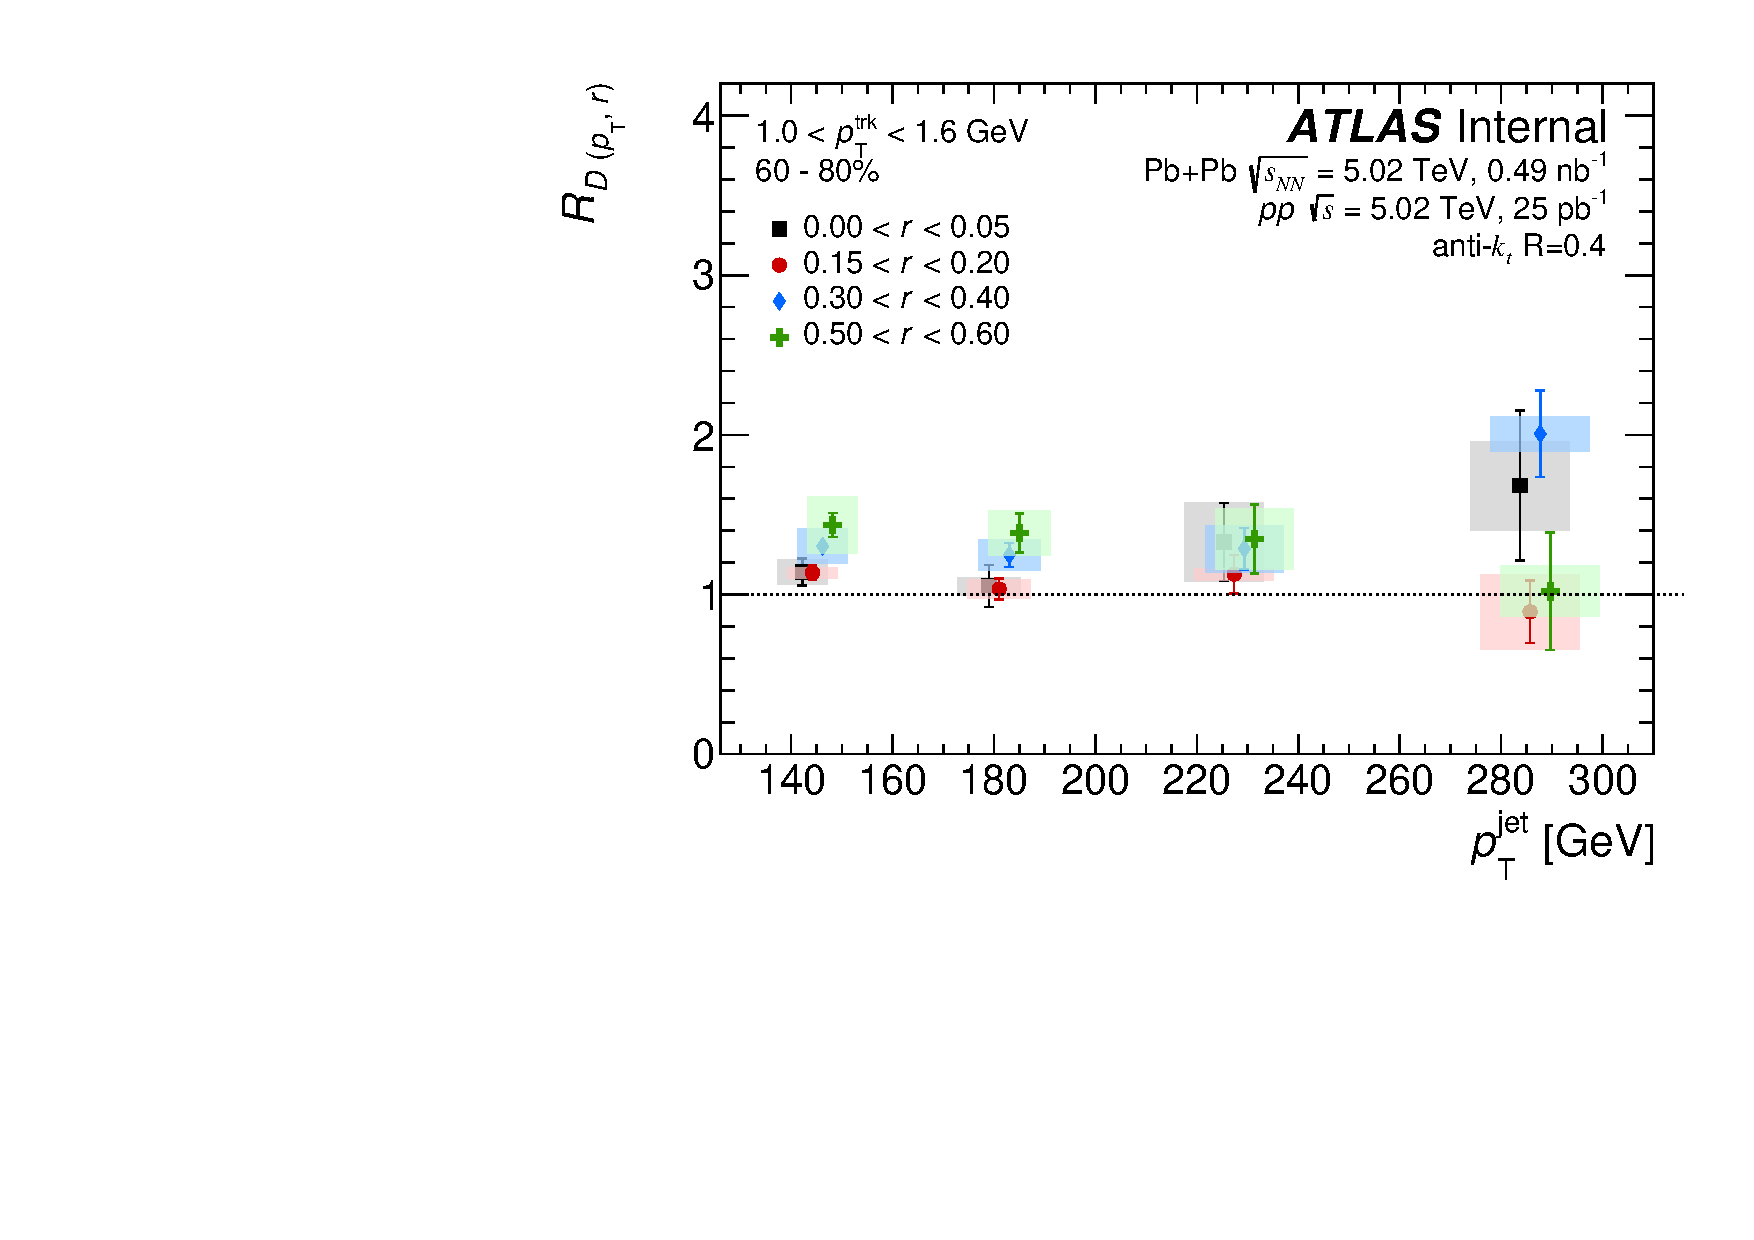
\includegraphics[width=0.45\textwidth]{results/RDpT_jetpt_trk2_cent5} \\
%	 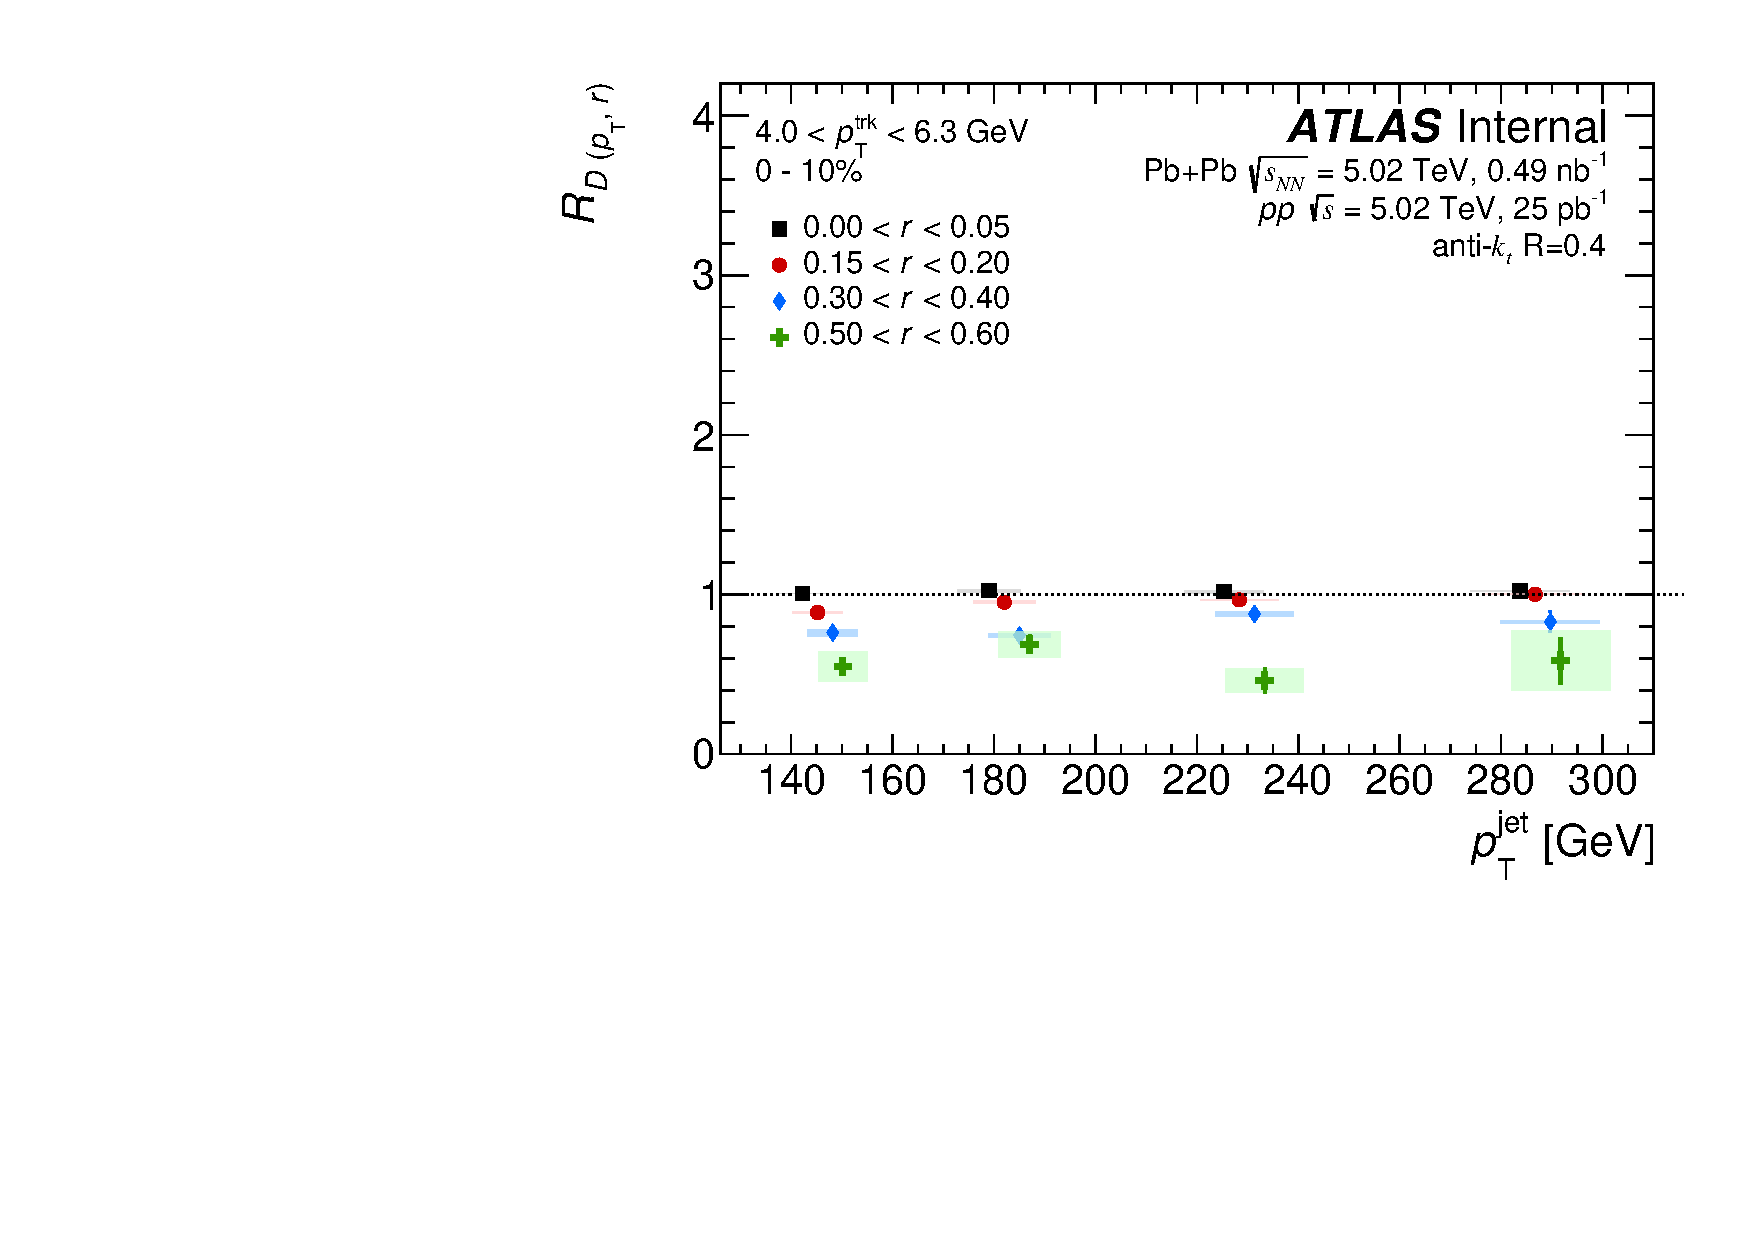
\includegraphics[width=0.45\textwidth]{results/RDpT_jetpt_trk5_cent0} &
%	 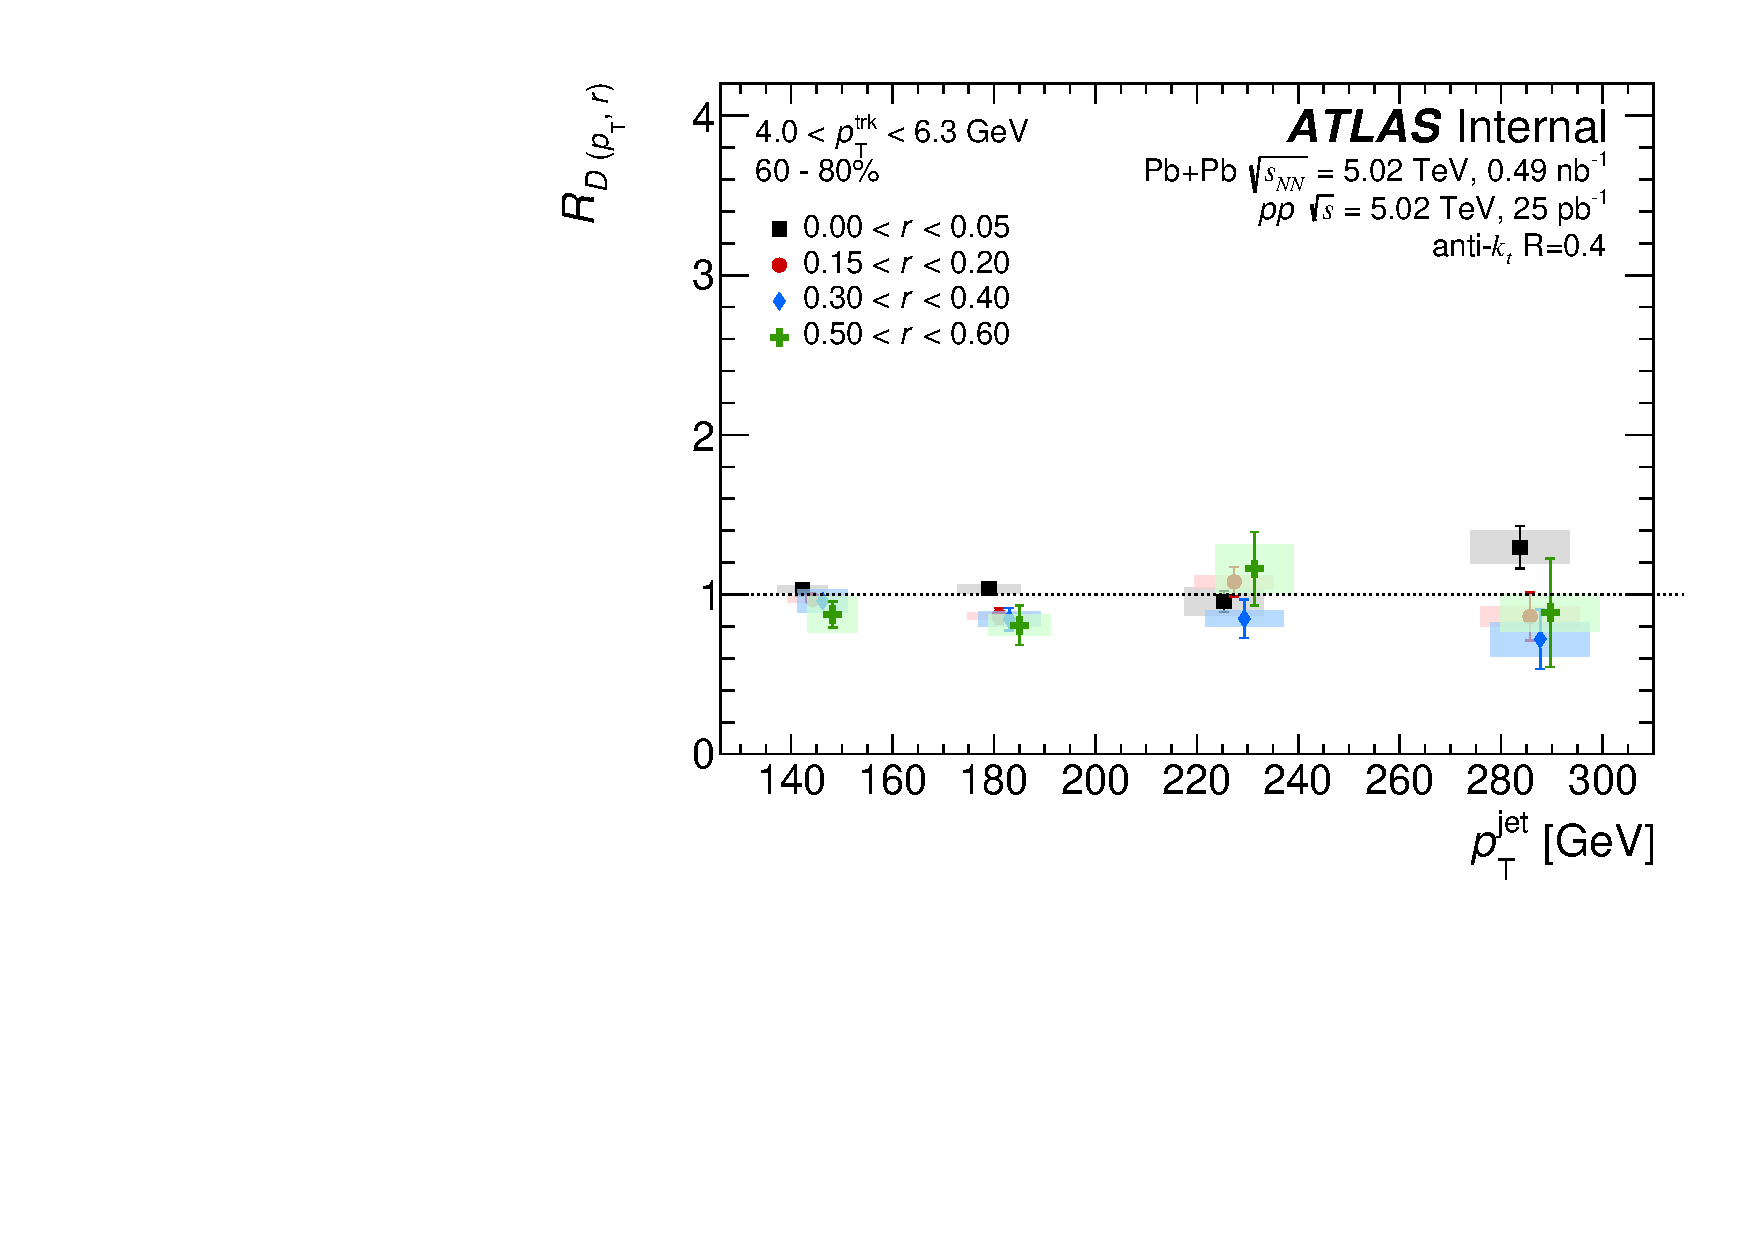
\includegraphics[width=0.45\textwidth]{results/RDpT_jetpt_trk5_cent5} \\
%\end{tabular} }
%   \caption{\RDptr as a function of \ptjet\ for charged particles with $1.0 < \pt < 1.6$ GeV (top) and $4.0 < \pt < 6.3$ GeV (bottom) at different distances from the jet axis and in 0--10\% central (left) and 60--80\% peripheral (right) \pbpb\ collisions. The vertical bars on the data points indicate statistical uncertainties while the shaded boxes indicate systematic uncertainties. The widths of the boxes are not indicative of the bin size and the points are shifted horizontally for better visibility.}
%      \label{fig:rdptr_jetpt}
%\end{figure}

%\begin{align}
%\frac{\int_1^{4} \Dpt_{\mathrm{PbPb}} \fd \pt }{\int_1^{4.2} \Dpt_{\mathrm{pp}} \fd \pt } &\qquad \frac{\int_1^{4} \Dpt_{\mathrm{PbPb}} \pt \fd \pt }{\int_1^{4} \Dpt_{\mathrm{pp}} \fd \pt } \\
%\int_1^{4} \Dpt_{\mathrm{PbPb}} - \Dpt_{\mathrm{pp}} \fd \pt  &\qquad \int_1^{4} \Dpt_{\mathrm{PbPb}} - \Dpt_{\mathrm{pp}} \pt \fd \pt \\
%\frac{\int_0^r \int_1^{4} \Dpt_{\mathrm{PbPb}} \fd \pt \fd r' }{\int_0^r \int_1^{4.2} \Dpt_{\mathrm{pp}} \fd \pt \fd r' } &\qquad \frac{\int_0^r \int_1^{4} \Dpt_{\mathrm{PbPb}} \pt \fd \pt \fd r'}{\int_0^r \int_1^{4} \Dpt_{\mathrm{pp}} \fd \pt \fd r'} \\
%\int_0^r \int_1^{4} \Dpt_{\mathrm{PbPb}} - \Dpt_{\mathrm{pp}} \fd \pt \fd dr'  &\qquad \int_0^r \int_1^{4} \Dpt_{\mathrm{PbPb}} - \Dpt_{\mathrm{pp}} \pt \fd \pt \fd dr'
%\end{align}

These measurements show that the excess of particles with $\pt <$~4.0~\GeV\ observed in~\cite{Aaboud:2018hpb} extends
outside the \RFour\ jet cone.
The measured dependence of \RDptr\ suggests that the energy lost by jets through the jet quenching process is being transferred to particles with $\pt <$~4.0~\GeV\ at larger radial distances from the jet axis. 
%This is qualitatively consistent with theoretical calculations \mbox{\cite{Blaizot:2014ula}}.
Additionally, these observations are in agreement with the previous measurement of jet fragmentation functions \cite{Chatrchyan:2014ava, Sirunyan:2018jqr, Aaboud:2017bzv, PhysRevC.98.024908} and may indicate the dependence of the response of the hot dense matter to the momentum of a jet passing through it. 


\FloatBarrier
